\documentclass[oneside,11pt,dvipsnames]{book}

\usepackage[utf8]{inputenc}
\usepackage[T1]{fontenc}
\usepackage[margin=1.5in]{geometry}
\usepackage{amsmath,amssymb,amsthm}
\usepackage{soul}
% \usepackage[small,compact]{titlesec} %very powerful
\usepackage[most]{tcolorbox}
% \setsecnumdepth{subsection}
% \setcounter{tocdepth}{3}
\usepackage{multirow,multicol}
\usepackage{enumitem}
\usepackage{epigraph}
\usepackage{cite}
\usepackage{caption}
\captionsetup{font=small}
\usepackage{graphicx}
\usepackage{pdfpages}
\usepackage{hyperref}
\usepackage{wrapfig}
\setlength\intextsep{0pt} % remove extra space above and below in-line float
\usepackage{hyperref}
\hypersetup{
  colorlinks,
  citecolor=black,
  filecolor=black,
  linkcolor=blue,
  urlcolor=blue,
}
\usepackage{booktabs}
\usepackage[linesnumbered,ruled,vlined]{algorithm2e}
\usepackage{listings}
\lstset{basicstyle=\ttfamily\scriptsize,
  language=python,
  morekeywords={assert},
  keywordstyle=\color{blue},
  commentstyle=\color{magenta},
  numbers=none,
  mathescape,
  stepnumber=1,
  numbersep=8pt,
  tabsize=4,
  showspaces=false,
  showstringspaces=false,
  emph={},
  emphstyle=\color{red}\bfseries
}
\definecolor{keywords}{RGB}{0,35,197}
\definecolor{comments}{RGB}{19,121,0}
\definecolor{highlight}{RGB}{255,255,102}

\lstdefinelanguage{Alloy}
	{
	basicstyle=\small\sffamily, %\normalsize\sffamily,
	%\footnotesize\sffamily, %\small\sffamily, %\scriptsize\sffamily,
	morekeywords={and,let,Int,then,check,module,run,sig,abstract,extends,one,lone,some,set,open,module,assert,not,fact,pred,all,no,fun,in,implies,else,no,or},
	numbers=left,					% where to put the line-numbers
	numberstyle=\scriptsize,			%\tiny,      % the size of the fonts that are used for the line-numbers
	stepnumber=1,					% the step between two line-numbers. If it's 1 each line will be numbered
	numbersep=7pt,%5pt,				% how far the line-numbers are from the code
	backgroundcolor=\color{white},	% choose the background color. You must add \usepackage{color}
	showspaces=false,				% show spaces adding particular underscores
	showstringspaces=false,			% underline spaces within strings
	showtabs=false,					% show tabs within strings adding particular underscores
	frame=b, %tb,				%none, %single % adds a frame around the code
	tabsize=2,						% sets default tabsize to 2 spaces
	captionpos=b,					% sets the caption-position to bottom
	breaklines=true,					% sets automatic line breaking
	breakatwhitespace=false,			% sets if automatic breaks should only happen at whitespace
	numberbychapter=false,
	aboveskip=0.25em,
	belowskip=0.25em,
	escapeinside={(*@}{@*)},
	xleftmargin=1.5em,
	escapeinside={(*@}{@*)},
	    keywordstyle=\color{keywords}\bfseries,
	   commentstyle=\color{comments},
	    morecomment=[l][\color{comments}]{//},
	    morecomment=[l][\color{comments}]{--},
	   stringstyle=\color{strings}
}

\usepackage{tikz}
\usetikzlibrary{calc}
\usepackage{xcolor}

\usepackage{anyfontsize}
\usepackage{sectsty}

\usepackage{etoolbox}

\newtoggle{usesol}
\settoggle{usesol}{false} % not sol version
\newcommand{\sol}[1]{\iftoggle{usesol}{\textbf{Sol:} #1}{}}
\newcommand{\notsol}[1]{\nottoggle{usesol}{#1}{}}
\newcommand{\solite}[2]{\iftoggle{usesol}{#1}{#2}}

\usepackage[makeroom]{cancel}

\newtcolorbox{mybox}{
  enhanced,
  boxrule=0pt,frame hidden,
  borderline west={2pt}{0pt}{green!75!black},
  colback=green!10!white,
  sharp corners
}

\newenvironment{commentbox}[1][]{
  \small
  \begin{mybox}
    {\small \textbf{#1}}
  }{
  \end{mybox}
}

\newtcolorbox{myhistorybox}{
  enhanced,
  boxrule=0pt,frame hidden,
  borderline west={2pt}{0pt}{red!75!black},
  colback=blue!10!white,
  sharp corners
}


\newenvironment{historybox}[1][]{
  \small
  \begin{myhistorybox}
    {\small \textbf{#1}}
  }{
  \end{myhistorybox}
}


\newtcolorbox{mycenterdisplay}{
    colframe=green!50!black, colback=gray!5!white, boxrule=0.5mm, sharp corners
}

\newenvironment{centerdisplay}[1][]{
  \small
  \centering
  \begin{mycenterdisplay}
    {\small \textbf{#1}}
  }{
  \end{mycenterdisplay}
}

\newtheorem{definition}{Definition}[section]
\newtheorem{theorem}{Theorem}[section]

\renewcommand{\implies}{\Rightarrow}

\renewcommand{\figurename}{Fig.}
\renewcommand{\tablename}{Tab.}
\def\Section{\S}
\renewcommand{\figureautorefname}{Fig.}
\renewcommand{\tableautorefname}{Tab.}
\makeatletter
\renewcommand{\chapterautorefname}{\S\@gobble}
\renewcommand{\sectionautorefname}{\S\@gobble}
\renewcommand{\subsectionautorefname}{\S\@gobble}
\renewcommand{\appendixautorefname}{\S\@gobble}
%\@addtoreset{chapter}{part}
\makeatother

\newcommand{\mycomment}[3][\color{blue}]{{#1{{#2}: {#3}}}}
\newcommand{\tvn}[1]{\mycomment{TVN}{#1}}{}
\newcommand{\red}[1]{{\color{red}{#1}}}
\newcommand{\code}[1]{\texttt{#1}}

\begin{document}

%\pagestyle{empty}
\begin{tikzpicture}[overlay,remember picture]

    % Background color
    \fill[
    black!2]
    (current page.south west) rectangle (current page.north east);

    % Rectangles
    \shade[
    left color=Dandelion,
    right color=Dandelion!40,
    transform canvas ={rotate around ={45:($(current page.north west)+(0,-6)$)}}]
    ($(current page.north west)+(0,-6)$) rectangle ++(9,1.5);

    \shade[
    left color=lightgray,
    right color=lightgray!50,
    rounded corners=0.75cm,
    transform canvas ={rotate around ={45:($(current page.north west)+(.5,-10)$)}}]
    ($(current page.north west)+(0.5,-10)$) rectangle ++(15,1.5);

    \shade[
    left color=lightgray,
    rounded corners=0.3cm,
    transform canvas ={rotate around ={45:($(current page.north west)+(.5,-10)$)}}] ($(current page.north west)+(1.5,-9.55)$) rectangle ++(7,.6);

    \shade[
    left color=orange!80,
    right color=orange!60,
    rounded corners=0.4cm,
    transform canvas ={rotate around ={45:($(current page.north)+(-1.5,-3)$)}}]
    ($(current page.north)+(-1.5,-3)$) rectangle ++(9,0.8);

    \shade[
    left color=red!80,
    right color=red!80,
    rounded corners=0.9cm,
    transform canvas ={rotate around ={45:($(current page.north)+(-3,-8)$)}}] ($(current page.north)+(-3,-8)$) rectangle ++(15,1.8);

    \shade[
    left color=orange,
    right color=Dandelion,
    rounded corners=0.9cm,
    transform canvas ={rotate around ={45:($(current page.north west)+(4,-15.5)$)}}]
    ($(current page.north west)+(4,-15.5)$) rectangle ++(30,1.8);

    \shade[
    left color=RoyalBlue,
    right color=Emerald,
    rounded corners=0.75cm,
    transform canvas ={rotate around ={45:($(current page.north west)+(13,-10)$)}}]
    ($(current page.north west)+(13,-10)$) rectangle ++(15,1.5);

    \shade[
    left color=ForestGreen,
    rounded corners=0.3cm,
    transform canvas ={rotate around ={45:($(current page.north west)+(18,-8)$)}}]
    ($(current page.north west)+(18,-8)$) rectangle ++(15,0.6);

    \shade[
    left color=ForestGreen,
    rounded corners=0.4cm,
    transform canvas ={rotate around ={45:($(current page.north west)+(19,-5.65)$)}}]
    ($(current page.north west)+(19,-5.65)$) rectangle ++(15,0.8);

    \shade[
    left color=OrangeRed,
    right color=red!80,
    rounded corners=0.6cm,
    transform canvas ={rotate around ={45:($(current page.north west)+(20,-9)$)}}]
    ($(current page.north west)+(20,-9)$) rectangle ++(14,1.2);



    % Title
    \node[align=center] at ($(current page.center)+(0,-5)$)
    {
    {\fontsize{32}{1} \selectfont {{\textbf{S}oftware \textbf{A}nalysis and \textbf{F}ormal r\textbf{E}asoning}}}\\[0.5in]

    {\fontsize{14}{19.2} \selectfont \textcolor{ForestGreen}{ \bf ThanhVu (Vu) Nguyen}}\\[0.1in]
    \today{} (latest version available on  \href{https://nguyenthanhvuh.github.io/class-oo/safe.pdf}{nguyenthanhvuh.github.io/class-oo/safe.pdf})
    };
    \end{tikzpicture}


\chapter*{Preface}



\newpage
\tableofcontents


% \chapter{Introduction}\label{sec:intro}

% This book will show you the fundamentals of developing high-quality software using a modern \textbf{object-oriented programming} (OOP) approach.  The goal is to develop programs that are reliable, efficient, and easy to understand and maintain.  We will use \emph{Python} for demonstration, but the concepts can be applied to any object-oriented programming language such as Java, C++, and Rust.


% \section{Decomposition}\label{sec:decomposition}

% As the size of a program increases, it becomes essential to \emph{decompose} the program into smaller, independent programs (or functions or modules). This decomposition process allows for easier management of the program, especially when multiple developers are involved.   This makes the program easier to understand and maintain.




% %\subsection{Decomposition}

% Decomposition is the process of breaking a complex program into smaller, independent, more manageable programs, i.e., ``divide and conquer''. It allows programmer to focus on one part of the problem at a time, without worrying about the rest of the program.

% \paragraph{Example} \autoref{ex:mergesort} shows a Python implementation of \emph{Merge Sort}, a classic example of problem decomposition. It breaks the problem of sorting a list into simpler problems of sorting smaller lists and merging them.

% \begin{figure}[t]
% \begin{lstlisting}[multicols=2]
% def merge_sort(lst):
%     if len(lst) \le 1:
%         return lst

%     mid = len(lst) // 2
%     left = merge_sort(lst[:mid])
%     right = merge_sort(lst[mid:])
%     return merge(left, right)







% def merge(left, right):
%     result = []
%     i = j = 0

%     while i < len(left) and j < len(right):
%         if left[i] < right[j]:
%             result.append(left[i])
%             i += 1
%         else:
%             result.append(right[j])
%             j += 1

%     result.extend(left[i:])
%     result.extend(right[j:])
%     return result
% \end{lstlisting}
%  \caption{Decomposition example: Mergesort}\label{ex:mergesort}
% \end{figure}


% A large part of this book focuses on \emph{abstraction}, a key concept in OOP that allows programmers to hide the implementation details and focus on the essential features. By decoupling the \textbf{what} (the  behavior specification) from the \textbf{how} (the actual implementation), programmers could focus on higher-level design and reuse code more effectively.
% % In an OOP language such as Python, you can abstract problems by creating functions, classes, and modules that hide the underlying implementation details.


% \begin{figure}[t]
% \begin{lstlisting}
% class Mammal:
%     def __init__(self, name):
%         self.name = name

%     def speak(self): pass

% class Dog(Mammal):
%     def speak(self): 
%         """
%         EFFECTS: Return the sound of a dog.
%         """
%         return "Woof!"

% class Cat(Mammal):
%     def speak(self):
%         """
%         EFFECTS: Return the sound of a dog.
%         """
%         return "Meow!"
    

% \end{lstlisting}
%  \caption{Decomposition example: Mergesort}\label{ex:mammal}
% \end{figure}


% \paragraph{Example} \autoref{ex:mammal} demonstrates an abstraction for different types of mammals. Mammals such as Dog and Cat share common behaviors such as making noise (speak). We can create a class \code{Mammal} that defines these common behaviors, and then subclasses \code{Dog} and \code{Cat} that inherit from \code{Mammal} and define their own unique behaviors.  These classes are abstract data types (ADT) that allow us to work with mammals. Also notice the specification (e.g., \code{EFFECTS}) in the comments that describe what the method does, not how it does it.




\part{Abstraction and Specification}

In this part of the book, we will focus on program abstraction via specifications. Specifications allow developers to describe the behavior of a program without revealing its implementation details, thus making the program easier to understand and maintain and also more general, i.e., can use different algorithms or data structures.

We will start with \emph{procedural abstraction} (\autoref{chap:procedural-abstraction}), which is on the specification of functions and methods. We will then move on to \emph{data abstraction} (\autoref{chap:adt}),  which is on the specification of abstract data types (ADTs) that encapsulate data and operations on that data.

\chapter{Procedural Abstraction and Specification}\label{chap:procedural-abstraction}


Abstraction is a key concept in software development that allows programmers to hide the implementation details and focus on the essential features. By decoupling the \textbf{what} (the  behavior specification) from the \textbf{how} (the actual implementation), programmers could focus on higher-level design and reuse code more effectively.

\emph{Procedural abstraction} hides implementation details from program functions or procedures. This makes the function more general and reusable, and the program easier to understand and maintain. The most common kind of abstraction that is familiar to all programmers is \emph{parameterization}, which allows a function to take in different input values. For example, the \code{cal\_area} function in \autoref{ex:abs-parameterization} calculates the area of a rectangle given its length and width, which are passed as parameters. 


\begin{figure}[h]
    \begin{lstlisting}
    def cal_area(length: int , width:int ) -> int;
        return length * width

    # can be used with different values for length and width.
    area1 = cal_area(5, 10)
    area2 = cal_area(7, 3)
\end{lstlisting}
\caption{Example: Abstraction by Parameterization}\label{ex:abs-parameterization}
\end{figure}

Another type of abstraction is through \emph{specification}, which is less common  but is crucial for creating and maintaining high-quality software (e.g., for API documentation). Specification defines what the function does (e.g., sorting), instead of how it does it (e.g., using quicksort or mergsort algorithms, implemented in C++). For example, from its specification in the comment, we know that the \code{exists} function in \autoref{ex:abs-specification} returns true if the \code{target} item is found in a list of sorted \code{items}. We do not need to know or care about the search algorithm used.
\begin{figure}
\begin{lstlisting}
    def exists(items:List[int], target:int) -> bool:
        """
        Find an item in a list of sorted items.

        Requires: List of sorted items
        Effects: Returns True if the target is found, False otherwise.
        """
        ...
\end{lstlisting}
\caption{Abstraction by Specification}\label{ex:abs-specification}
\end{figure}


By defining a function's behavior through specifications, developers can implement the function in different ways as long as it fulfills the specifications. Similarly, the user can use the function without knowing the implementation details. In this chapter, we will focus on procedural specification and how construct and formalize specifications for functions and methods\footnote{We use the terms \emph{function}, \emph{method}, and \emph{procedures} interchangeably.}.

\section{Specifications}\label{sec:specifications}

%Specifications can be written in either \emph{formal} or \emph{informal languages}. Formal specifications have the advantage of being precise and unambiguous. However we often use informal specifications such as comments to describe program behaviors and properties (e.g., the \code{exists} example in \autoref{ex:abs-specification}).  In many cases we use a mixture of both, e.g., using formal specifications using logical formulas or assertions and informal specifications using comments.


%Specifications allow developers to abstract programming details, describing what the program does without revealing how it does it. 


%Note that a specification is not a programming language or a program. Thus, our specifications won’t be written in code, e.g., in Python or Java.

%\subsection{Specifications of a Function}\label{sec:spec-function}
%3.3 Liskov

The description of a function is captured through its \emph{header} and \emph{specification}.
The header gives the signature of the function, including its name, parameters, and return type. The specification describes the function's behavior, including its preconditions and postconditions.

\paragraph{Header} Function header, also called the \emph{signature} of a function, is the first line of the function definition. It provides the \emph{name} of the function, the number, order, and types of its \emph{parameters} (inputs), and the type of its return value (output). For instance, the headers for functions \code{cal\_area} in \autoref{ex:abs-parameterization} and \code{exist} in \autoref{ex:abs-specification} are: 

\begin{lstlisting}
def exists(items: list) -> bool: ...
def calc_area(length: float, width: float) -> float: ...
\end{lstlisting}


\begin{commentbox}{\textbf{Type Hinting}: }
    Python does not require specifying the types of parameters and return values. However, in more recent versions of Python, you can use \emph{type hinting} to specify the types of parameters and return values as shown above. While type hinting is not enforced by Python, it is useful for documentation and code readability. We will use type hinting in this book to make the code more readable. 
\end{commentbox}


Note that in a language like Java, the header can also indicate \emph{exceptions} that the method may throw, e.g., 

\begin{lstlisting}[language=Java]
public boolean exists(List<Integer> items) throws Exception { ... }
\end{lstlisting}

However, function header alone is not sufficient to describe the behavior of a function. We need to provide a more detailed description of the function's behavior, which is done through the \emph{specification}.

\subsection{Specification}

The specification of a function defines the behavior of the function.  It includes: \emph{preconditions} (also called the ``Requires'' clause) and \emph{postconditions} (also called the ``Effects'' clause). Preconditions describe the conditions that must be true before the function is called. Often these are constraints or assumptions about the input parameters. If there are no preconditions, the clause is often written as \code{None}.

Postconditions, under the assumption that the preconditions are satisfied, describe the conditions that will be true after the function is called. Postconditions state the expected results or outcomes of the function. Moreover, they often describe the relationship between the inputs and outputs.


\begin{lstlisting}
def calc_area(length: float, width: float) -> float:
    """
    Calculates the area of a rectangle given its length and width.

    Reqires: None
    Effects: The area of the rectangle which is the product of the length and width.
    """
    ...
\end{lstlisting}

The clauses are usually written as \emph{comments} above the function definition. For example, the specification of the \code{calc\_area} function in \autoref{ex:abs-parameterization} has (i) no preconditions and (ii) the postcondition that the function returns the area of a rectangle given its length and width.  Similarly, the \code{exists} function in \autoref{ex:abs-specification} has the specification that given a list of sorted items (precondition), it returns true if the item is found in the list, and false otherwise (postcondition).  Notice how the specification is written in plain English, making it easy to understand for both developers and users of the function.


\subsection{Modifies} Another clause that might appear in a function specification is \emph{modifies}, which describes variables that the function can change. Often, these would be the input parameters, e.g., the function can modify the input list or data structure passed to it. However, this could also be other variables such as global variables like counters or flags.
A main use of the \emph{modifies} clause is to reveal and avoid \emph{side effects}.

For example, the \code{add\_to\_list} function below modifies the input list and the \code{dirty\_bit} flag.

\begin{lstlisting}

dirty_bit = False    
def add_to_list(input_list: List[int], value: int) -> None:
    """
    Adds a value to the input list.

    Requires: None
    Effects: Value is added to the input list.
    Modifies: the input list, dirty_bit
    """
    ...
\end{lstlisting}

\subsection{Invariants and Assertions}\label{sec:invariants}

\paragraph{Invariants} A related concept to pre- and postconditions is \emph{invariants}, which are conditions that must be true at all times during the execution of the function. For example, the \code{calc\_area} function in \autoref{ex:abs-parameterization} can have an invariant that the length and width are always positive.


Common invariants include \emph{loop invariants}, which are conditions that must be true at the beginning and end of each iteration of a loop (\autoref{chap:loop-invariants}), and \emph{representation invariants} (rep invariants), which are conditions that must be true for the internal state of a class (\autoref{chap:adt}). An example of repr invariants for a class representing a binary search tree is that the left child is less than the parent and the right child is greater than the parent.

\begin{commentbox}[Invariants Examples]
    Examples of loop invariants include a \textbf{bubble sort} implementation might have an invariant that \emph{after each complete pass through the array, the last $k$ elements are in their final sorted positions}. This shows that with every iteration, the largest unsorted element ``bubbles up'' to its correct position.
    For binary search, a loop invariant could be that \emph{if the target value is in the list, it is in the range of the left and right indices}. This shows that after each iteration (which changes the left and right indices), the target value is still in the list.
    \\

    For repr invariants, a class representing a binary search tree (BST) might have an invariant that the left child is less than the parent and the right child is greater than the parent. This ensures that the BST is correctly structured and is not affected by any operations on the tree.
\end{commentbox}


Unlike specifications, which should not reveal implementation details, invariants can involve implementation details.  For example the condition $x==0$ is True in line 7 of the file \code{safe.c} or that the array used to represent the binary search tree needs to have a certain property.  Moreover, invariants are often checked during program execution, i.e., runtime checking, as assertions described next.


\paragraph{Assertions} Assertions are a common way to check at the runtime constraints (code \texttt{expressions}) that should be true at a certain point in the program. Unlike pre and postconditions and invariants that are written as comments, assertions are often written as code and are checked during program execution. For example, the \code{calc\_area} function in \autoref{ex:abs-parameterization} can have several assertions as follows:

\begin{lstlisting}
def calc_area(length: float, width: float) -> float:
    """
    Requires: ... 
    Effects: ...
    """
    ...
    assert length > 0 and width > 0  # check preconditions

    # calculate the area and store it in res
    ... 

    assert res > 0  
    return res 
\end{lstlisting}



Assertions can be used to check the preconditions, postconditions, invariants, or any other conditions that the programmer believes should be true.  If an assertion is false, an exception is raised, indicating a bug in the program (e.g., see~\autoref{fig:assertion}). Thus, assertions are useful for debugging and testing the program. 

\begin{figure}
    \centering
    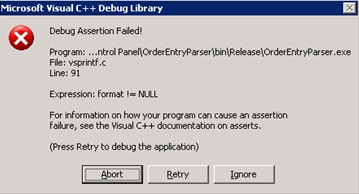
\includegraphics[width=0.55\textwidth]{figs/assertions.jpg}
    \caption{Assertion violation. The expression \code{format!=NULL} fails on line 91 of the file \code{vsprintf.c}.}\label{fig:assertion}
    \caption{The expression }
\end{figure}

\subsection{API} 

\section{Designing Specifications}\label{sec:design-specifications}
%Liskov 3.5

To have well-designed and effective specifications, it is important to consider several factors. These include the \emph{strength} of the pre- and post-conditions, whether the function is \emph{total} or \emph{partial}, and \emph{avoiding implementation details} in the specification.

\subsection{Weakest Pre-conditions}\label{sec:weakest-preconditions}
For pre-conditions, we want as weak a constraint as possible to make the function more versatile, allowing it to handle a larger class of inputs.
Logically, a condition $x$ is weaker than another if it is \emph{implied} by the other $y$, i.e.,  $y \implies x$, or that $x$'s constraints are a superset of $y$'s. For example, the condition $x \le 10$ is weaker than $x \le 5$ (because everything that is less than 5 is also less than 10). Thus a function that works with $x \le 10$ is better than one that works with $x \le 5$ because it can handle more inputs.

As another example the input list is not sorted is weaker than the list is sorted (which is weaker than the list that is both sorted and has no duplicates). Thus a function that can handle any list is better than one that can only handle sorted lists.

The \emph{weakest} precondition is \emph{True}, which indicates no constraints on the input.

\subsection{Strongest Post-conditions}\label{sec:strongest-postconditions}

In contrast, for post-conditions, we want as strong a condition as possible to ensure that the function behaves as expected. A condition $y$ is stronger than another condition $x$ if $y$ implies $x$, i.e., $y \implies x$, or that $y$'s constraints are a strict subset of $x$'s.
For example, the condition $x \le 5$ is stronger than $x \le 10$ (because everything that is less than 5 is also less than 10) or that the input list is sorted is stronger than the list is not sorted.   The reason stronger is better for postcondition is that it describes the expected behavior more precisely, e.g., a person who's under 5 feet is more precise than a person who's under 10 feet.

\subsection{Total vs Partial Functions}\label{sec:total-partial-function}

A function is \emph{total} if it is defined for all legal inputs; otherwise, it is \emph{partial}. Thus a function with no precondition (weakest precondition) is total.  

Total functions are \emph{preferred} because they can be used in more situations, especially when the function is used publicly or in a library where the user may not know the input constraints. Partial functions can be used when the function is used internally, e.g., a helper or auxiliary function and the caller is knowledgeable and can ensure its preconditions are satisfied.

For example, functions \code{calc\_area} in \autoref{ex:abs-parameterization} and \code{add\_to\_list} in \autoref{ex:abs-specification} are total because they can be called with any input. The \code{exists} function in \autoref{ex:abs-specification} is partial because it only accepts sorted lists.


\paragraph{Turning Partial Functions into Total Functions} We can often turn a partial function into a total function in two steps. 
\begin{enumerate}

    \item Move preconditions into postconditions and (in the postconditions) specify the expected behavior when the precondition is not satisfied, e.g., when invalid input \code{X} occurs, throws an exception \code{Y} 

    \item Modify the function to satisfy the new specification (specifically, to satisfy the new postcondition).  In other words, add code to handle the cases when the preconditions are not satisfied. 
\end{enumerate}

For example, the \code{exists} function in \autoref{ex:abs-specification} is turned into the total function shown in \autoref{ex:abs-total}.

\begin{figure}
\begin{lstlisting}
def exists(items: List[int], target: int) -> bool:
    """
    Find an item in a list of sorted items.

    Pre: True
    Post: If the input items are not sorted, raise an exception.
          Return True if the item is found, False otherwise.


    """

    if not is_sorted(items):
        raise Exception(...)
\end{lstlisting}
\caption{Total Specification for the program in \autoref{ex:abs-specification}}\label{ex:abs-total}
\end{figure}



\subsection{Avoid Implementation Details in Specifications}

A specification should not include any implementation details, such as the algorithm used or the data structures employed. This improves flexibility as it allows the function to be implemented in different ways as long as it satisfies the specification. For example, the \code{exists} function in \autoref{ex:abs-specification} does not specify the search algorithm used to find the item in the list.

Some common examples to avoid include: the mentioning of specific data structures (e.g., arrays, indices), algorithms (e.g., quicksort or mergesort), and exceptions (e.g., related to IndexError). Also avoid specifications mentioning indices because this implies the use of arrays.

\section{Under- vs Over-Specifications}

From what we have seen, we prefer specifications that balance both precision (postcondition) and flexibility (e.g., precondition, no implementation details). We want to avoid over and under-specifications.

\subsection{Over-Specification} 

An over-specified specification includes unnecessary constraints or implementation details that restrict the function's flexibility. For example, precondition that the input must be a list instead of iterable collections or include the use of specific algorithms or data structures. Over-specification makes the function less flesible and code less reusable.

\paragraph{Example: sorting function} Taking as input a list of integers (precondition) and returning a list that is a permutation of the input list in non-decreasing order using quicksort (postcondition). 

This is over-specified because it restricts the data structure to list and the sorting choice to quicksort (which has a worst case of $O(n^2)$).
A better spc would be take as input a collection of comparable elements and return a collection that is a permutation of the input collection in non-decreasing order. 


\subsection{Under-Specification}

An under-specified specification does not define the expected behavior of the function precisely. For example, failing to specify potential outputs or edge cases. Under-specification can cause incorrect implementation.

\paragraph{Example: Search for a number from a sorted list} Taking as input a list of numbers and a target number and returning the location of the target number in the list.  This is under-specified because it doesn't specify what happens if the target is not found or if there are duplicates. A better specification would be to return the location of the target if it is found, raise an exception if the target is not found, and return the first location if there are duplicates.


\section{More Examples of Bad Specifications}

\begin{itemize}
    \item The function \texttt{find\_max} takes a list of elements (precondition) and returns the maximum element by iterating over the indices from 0 to n-1 (postcondition).
    \item The function \texttt{sort\_list} sorts a list of numbers (precondition) and uses quicksort to sort the list (postcondition).
    \item The function \texttt{exists} returns true if the target is found or raise IndexError if the target is not found (postcondition)
\end{itemize}

% \section{Formal Specifications}\label{sec:formal-specs}

% While informal specifications, e.g., as pre and post-conditions in comments, are easy to understand, they can be ambiguous and imprecise. Formal specifications, on the other hand, are precise and unambiguous, making them useful for complex systems or when the behavior must be precisely defined.

% %Examples of formal specifications include \emph{assertions} and \emph{preconditions} and \emph{postconditions} in languages like Java, C++, and Python. These are logical formulas that describe the expected behavior of the function. For example, the \code{calc\_area} function in \autoref{ex:abs-parameterization} can be specified formally as follows:


% \subsection{Specification Languages} 

% Several formal languages or notations are designed specifically for writing specifications. Some popular ones include: the Z notation and the Alloy language.  These languages are based  mathematical logic and set theory and are used to describe the behavior of a program in a precise and unambiguous way. 

% For example, an informal specification for a \code{login} function might be:

% \begin{lstlisting}
% def login(username: str, password:str) -> bool:
%     """
%     requires: username is a string, password is a string
%     ensures: if username and password are correct, return True
%     if username and password are incorrect, return False
%     if 3 failed attempts, lock user out
%     """
% \end{lstlisting}

% A formal specification for the same function Alloy might look like:

% \begin{lstlisting}[language=Alloy]
% // Signatures define objects in the login system
% sig User {
%     username: one String, // One username per user
%     password: one String  // One password per user
% }

% sig LoginSystem {
%     validUser: set User,  // Set of valid users in the system
%     failedAttempts: one Int // Number of failed login attempts
% }

% // Fact to initialize the system
% fact InitialState {
%     // Initially, the failedAttempts should be zero
%     LoginSystem.failedAttempts = 0
% }

% // Predicate for login
% pred login(u: User, pswd: String) {
%     // Check if the username and password match for the user
%     u.password = pswd
% }

% // Predicate for checking account lockout
% pred accountLocked {
%     LoginSystem.failedAttempts >= 3
% }

% // Assert that failed login attempts lead to lockout
% assert LockAfterThreeFailedAttempts {
%     all u: User, pswd: String | 
%         (login(u, pswd) and not accountLocked) implies LoginSystem.failedAttempts = 0
% }

% // See if the system works
% run LockAfterThreeFailedAttempts for 3 but 5 User, 3 LoginSystem    
% \end{lstlisting}    

% As can be seen, this formal specification is just like a program (potentially even more complex than the program itself). However, it is precise and unambiguous, and is useful for modeling and verifying complex systems.  The Alloy system can check for errors in the specification or prove that it satisfies certain properties.

%\chapter{Exception}
%Liskov 4 ,  but won't follow this because it talks about checked vs unchecked exceptions, which are not really applicable in Python.
\section{Exercise}

\subsection{Specification for Sorting}\label{exercise:specs-sort}
Write the specification for the generic \code{ascending\_sort} method below. The specification should include preconditions and postconditions.
\begin{lstlisting}
    def ascending_sort(my_list):
        # REQUIRES/PRE: 
        # EFFECTS/POST: 
        ...
\end{lstlisting}
    

\subsection{Specification for Merging Two Sorted List of Numbers}\label{exercise:specs-merge-lists}
Write the spec. for the function \code{merge\_sorted\_lists} that takes two sorted lists of (int) numbers and returns a single list in non-decreasing order that contains all the elements of the two input lists. The header of the function is given below.

\begin{lstlisting}
def merge_sorted_lists(lst1: List[int], lst2: List[int]) -> List[int]:
    """
    PRE/REQUIRES: 
    POST/EFFECTS: 
    """
    ...
\end{lstlisting}

\subsection{Specification of Binary Search}\label{exercise:specs-binary-search}

Come up with the specification for a \emph{binary search} implementation whose header is given below. Remember for precondition you want something as \emph{weak} as possible and for postcondition as \emph{strong} as possible. Note that binary search returns the \emph{location} (an non-neg integer) of the \code{target} value if found, and returns -1 if \code{target} is not found. 

\begin{lstlisting}
def binary_search(arr: List[int], target: int) -> int:
    """
    PRE/REQUIRES: 
    POST/EFFECTS: 
    """
    ... 
\end{lstlisting}


\subsection{Loan Calculator}\label{exercise:loan-calculator}    

Consider a function that calculates the number of months needed to pay off a loan of a given size at a fixed \emph{annual} interest rate and a fixed \emph{monthly} payment. For example, a \$100,000 loan at an 8\% annual rate would take 166 months to discharge at a monthly payment of \$1,000, and 141 months to discharge at a monthly payment of \$1,100. (In both cases, the final payment is smaller than the others; we round 165.34 up to 166 and 140.20 up to 141.) Continuing the example, the loan would never be paid off at a monthly payment of \$100, since the principal would grow rather than shrink.

\begin{itemize}


\item Define a function satisfying the following specification:

\begin{lstlisting}
def months(principal: int, rate: float, payment: int) -> int:
    """
    Calculate the number of months required to pay off a loan.
    
    param principal: Amount of the initial principal (in dollars)
    param rate: Annual interest rate (e.g., 0.08 for 8%)
    param payment: Amount of the monthly payment (in dollars)
    
    Requires/Pre: principal, rate, and payment all positive and 
    payment is sufficiently large to drive the principal to zero.
    Effects/Post: return the number of months required to pay off the principal
    """
\end{lstlisting}

\begin{itemize}
    \item The precondition is quite strong, which makes implementing the method easy. The key step in your calculation is to change the principal on each iteration with the following formula (which amounts to monthly compounding):
    \begin{lstlisting}
new_principal = old_principal * (1 + monthly_interest_rate) - payment
    \end{lstlisting}

    \item To make sure you understand the point about preconditions, your code is required to be \emph{minimal}. Specifically, if it is possible to delete parts of your implementation and still have it satisfy the requirements, you'll earn less than full credit.
\end{itemize}
\item \emph{Total} specification: Now change the specification to \emph{total} in which the postcondition handles violations of the preconditions using \emph{exceptions}. In addition, provide a new implementation \code{month} that satisfies the new specification.
\end{itemize}


\subsection{Partial and Total Specifications for \code{tail}}\label{exercise:tail}

Consider the following code:

\begin{lstlisting}
def tail(my_list):
     result = my_list.copy()
     result.pop(0)
     return result
\end{lstlisting}

\begin{itemize}
     \item What does the implementation of \code{tail} do in each of the following cases? You might want to see the \href{https://docs.python.org/3/tutorial/datastructures.html}{Python document} for \code{pop}.  How do you know: Running the code or reading Python document?
     \begin{itemize}
         \item \code{list = None}
         \item \code{list = []}
         \item \code{list = [1]}  
         \item \code{list = [1, 2, 3]}
     \end{itemize}
     \item Write a \emph{partial specification} that satisfies the given \code{tail} implementation
     \item Rewrite the specification to be \emph{total}. Use \emph{exceptions} as needed.
    \end{itemize}

\subsection{Partial and Total Functions}\label{exercise:partial-total}

\begin{enumerate}
    \item Write the \emph{partial} specifications for the below two functions.
    \item Modify the specifications to make the functions \emph{total}.
    \item Modify the \emph{implementations} of the two functions to satisfy the total specifications.
\end{enumerate}

Recall that specifications do not deal with types (which are specified by  function signatures and enforced by the type system of compiler/interpreter).  In other words, you do not need to worry about types here and can assume conditions about types are satisfied.

\begin{lstlisting}
def divide(a:float, b:float) -> float:
    """
    PRE:
    POST:
    """
    return a / b

def get_average(numbers: list[float]) -> float:
    """
    PRE:
    POST:
    """
    total = sum(numbers)
    return divide(total, len(numbers))
\end{lstlisting}



\sol{For \code{divide}, precond is \code{b} cannot be 0, postcond is the result is the division of \code{a} by \code{b}. For \code{get\_average}, precond is the list cannot be empty (which cause division by 0), postcond is the result is the average of the numbers in the list. To make them total, we throw an exception when the precond is violated.}


\subsection{Problems with Inheritance in OOP: Equality}\label{exercise:inheritance-equality}

Inheritance, which allows a class to inherit properties and methods from another class, is a key feature of OOP.
While this has many benefits, inheritance introduces certain unexpected kinds of issues for specifying desired properties and implementing them. This exercise will show you one of using the popular \emph{equals} method in OOP.

\begin{enumerate}
    \item First, look at the \href{https://docs.oracle.com/javase/8/docs/api/java/lang/Object.html#equals-java.lang.Object-}{Javadoc} to understand the behaviors \code{equals()} (while the specification is for Java, the idea is the same in Python).
    \begin{itemize}
        \item Specifically, read carefully the \emph{symmetric}, \emph{reflexive}, and \emph{transitive} properties of \code{equals()}.
        \item Ignore \emph{consistency}, which requires that if two objects are equal, they remain equal.
    \end{itemize}    
    \item For the \code{User} class in \autoref{ex:user}, does \code{equals()} satisfy the three equivalence relation properties? If not, what is the problem?
    \begin{itemize}
        \item Come up with several concrete test cases (e.g., create various \code{User} instances) to check the properties.
        \item If there is a problem, show the test case that demonstrates the problem.
        \item Explain why the problem occurs and come up with a fix.
    \end{itemize}
    \item Do the same analysis for the \code{SpecialUser} class in \autoref{ex:specialuser}.
    \end{enumerate}
    
    % 1. Is the given implementation of `equals()` in class `SpecialUser` satisfy the 3 equivalence relation properties? If not, what is the problem? Be concrete: find a specific object (test case!) that demonstrates the problem. How does *inheritance* makes `equals()` in class `SpecialUser` harder to get right?
    

\begin{figure}
\begin{lstlisting}
    class User:
        def __init__(self, name):
            self.name = name

        def __eq__(self, other):
            if not isinstance(other, User):
                return False
            return self.name == other.name
\end{lstlisting}
\caption{User class}\label{ex:user}
\end{figure}


\begin{figure}
\begin{lstlisting}
    class SpecialUser(User):
        """Don't do this until you've done with User"""

        def __init__(self, name, id):
            super().__init__(name)
            self.id = id

        def __eq__(self, other):
            if not isinstance(other, SpecialUser):
                return False
            return super().__eq__(other) and self.id == other.id
\end{lstlisting}
\caption{SpecialUser class}\label{ex:specialuser}
\end{figure}




\chapter{Abstract Data Type}\label{chap:adt}
%Liskov 5

%This chapter focuses on \emph{abstract data type} (ADT), a foundation of OOP and key concept in programming that allows developers to separate how data is implemented from how it behaves. Through ADT, programmers can create new data types relevant to their application. These ADTs consist of objects and associated operations.

In 1974, Barbara Liskov and Stephen N. Zilles introduced Abstract Data Types (\emph{ADTs}) in their influential paper ``Programming with Abstract Data Types'' as part of their work on the CLU programming language at MIT. ADTs changed software design by separating the specification of a data type from its implementation. This allows developers to define operations on a data structure without exposing the detailed implementation of data (e.g., calling \code{pop} to remove data from a \code{Stack} without knowing the internal details on how stack stores data). 

For her pioneering contributions to programming languages and system design, particularly on ADTs and CLU, Barbara Liskov was awarded the Turing Award in 2008. Today, ADTs are a cornerstone of all modern programming languages.

%The CLU language was the first to explicitly support ADTs using a construct called a cluster, which encapsulated both the data structure and the operations that acted on it. CLU also introduced several other innovative features like iterators, exceptions, and parameterized types, many of which influenced modern programming languages such as Java, Python, and C++. Though CLU never became widely used, the principles it introduced, especially ADTs, became foundational in software engineering, leading to more modular and reusable code.



%An ADT has two main components: \emph{parameterization} and \emph{specification}. Parameterization involves using parameters for flexibility, while specification means including operations as part of the data type, which abstracts away the underlying data representation. This ensures that even if the data structure changes, programs that rely on it remain unaffected, as they only interact with the operations rather than the data's internal structure.

%By abstracting data, developers can postpone decisions about data structures until they fully understand how the data will be used, leading to more efficient programs. ADT is also beneficial during program maintenance, as changes to the data structure affect only the type's implementation, not the modules using it.


\section{Specifications of an ADT}\label{sec:specs-adt}

The \emph{specification of an ADT} describe the operations and behaviors of the object, allowing users to interact with it only via methods, rather than accessing its internal representation. 
As with functions (\autoref{chap:procedural-abstraction}), the specification for an ADT defines its behaviors without being tied to a specific implementation (e.g., the internal data of an ADT).


\paragraph{Structure of an ADT} In a modern OOP language such as Python or Java, data abstractions are defined using \emph{classes}. Each class defines a name for the data type, along with its constructors and methods.

\begin{figure}
    \begin{lstlisting}
class DataType:
    """
    Overview: A brief description of the data type and its objects.
    """

    def __init__(self, ...):
        """
        Constructor to initialize a new object.
        """

    def method1(self, ...):
        """
        Method to perform an operation on the object.
        """
    \end{lstlisting}
    \caption{Abstract Data Type template}\label{ex:adt-template}
\end{figure}


\autoref{ex:adt-template} shows an ADT class template in Python. It consists of three main parts. The \emph{Overview} describes the abstract data type in terms of well-understood concepts, like mathematical models or real-world entities. For example, a stack could be described using mathematical sequences.
The Overview can also indicate whether the objects of this type are \emph{mutable} (their state can change) or \emph{immutable}.
The \emph{Constructor} initializes a new object, setting up any initial state required for the instance.
Finally, \emph{methods} define operations users can perform on the objects. These methods allow users to interact with the object without needing to know its internal representation. In Python, \code{self} is used to refer to the object itself, similar to \code{this} in Java or C++.

Note that as with procedural specification (\autoref{chap:procedural-abstraction}), the specifications of constructors and methods of an ADT do not include implementation details. They only describe what the operation does, not how it is done. Moreover, they are written in plain English as code comment.


\subsection{Example: \code{IntSet} ADT}

\autoref{ex:intset} gives the specification for an \code{IntSet} ADT, which represents unbounded set of integers. \code{IntSet} includes a constructor to initialize an empty set, and methods to insert, remove, check membership, get the size, and choose an element from the set. \code{IntSet} is also mutable, as it allows elements to be added or removed. \emph{mutator} \code{insert} and \code{remmove} are mutator methods and have a \code{MODIFIES} clause.  In contrast, \code{is\_in}, \code{size}, and \code{choose} are \emph{observer} methods that do not modify the object.

\begin{figure}
    \begin{lstlisting}
class IntSet:
    """
    Overview: IntSets are unbounded, mutable sets of integers.
    This implementation uses a list to store the elements, ensuring no duplicates.
    """

    def __init__(self):
        """
        Constructor
        EFFECTS: Initializes this to be an empty set.
        """
        self.els = []  # the representation (list)

    def insert(self, x: int) -> None:
        """
        MODIFIES: self
        EFFECTS: Adds x to the elements of this set if not already present.
        """
        if not self.is_in(x): self.els.append(x)
            
    def remove(self, x: int) -> int:
        """
        MODIFIES: self
        EFFECTS: Removes x from this set if it exists. Also returns       
        the index of x in the list.
        """
        i = self.find_idx(x)
        if i != -1:
            # Remove the element at index i
            self.els = self.els[:i] + self.els[i+1:]  
        return i

    def is_in(self, x: int) -> (bool, int):
        """
        EFFECTS: If x is in this set, return True. Otherwise False.
        """
        return True if find_index(x) != -1 else False

    def find_idx(self, x:int)->int:
        """
        EFFECTS: If x is in this set, return its index. Otherwise returns -1.
        """
        for i, element in enumerate(self.els):
            if x == element:
                return i
        return -1

    def size(self) -> int:
        """
        EFFECTS: Returns the number of elements in this set (its cardinality).
        """
        return len(self.els)

    def choose(self) -> int:
        """
        EFFECTS: If this set is empty, raises an Exception. 
        Otherwise, returns an arbitrary element of this set.
        """
        if len(self.els) == 0:
            raise Exception(...)
        return self.els[-1]  # Returns the last element arbitrarily

    def __str__(self) -> str:
        """
        Abstract function (AF) that returns a string representation of this set.
        EFFECTS: Returns a string representation of this set.
        """
        return str(self.els)
\end{lstlisting}
\caption{The IntSet ADT}\label{ex:intset}
\end{figure}

%\subsection{Example: \code{Polynomial} ADT}

\section{Implementing ADT}\label{sec:implementing-adt}

To implement an ADT, we first choose a \emph{representation} (\textbf{rep}) for its objects, then design constructors to initialize it correctly, and methods to interact with and modify the rep. 
For example, we can use a \code{list} (or vector) as the rep of \code{IntSet} in \autoref{ex:intset}. We could use other data structures, such as a \code{set} or \code{dict}, as the rep, but a list is a simple choice for demonstration.


To understanding and reasoning of the rep of an ADT, we use two key concepts: \emph{representation invariant} and \emph{abstraction function}.

\subsection{Representation Invariant (Rep-Inv)}\label{sec:rep-invs}
Because the rep data might not be related to the ADT itself (e.g., the list has different properties compared to a set), we need to ensure that our use of the rep is consistent with the ADT's behavior. 
To do this, we use \emph{representation invariant} (\textbf{rep-inv}) to specify the constraints for the rep to capture the behavior of the ADT.


For example, the rep-inv for a \emph{stack} is that the last element added is the first to be removed and the rep-inv for a \emph{binary search tree} (BST) is that the left child is less than the parent, and the right child is greater. 
The rep-inv for our \code{IntSet} ADT in \autoref{ex:intset} is that all elements in the list are unique integers. 
\begin{lstlisting}
    # Rep-inv:
    # els is not null, only contains integers and has no duplicates.
\end{lstlisting}

%[TODO: add after this semester] Note that unlike pre and post-conditions in function specifications that do not include implementation details, the rep-inv is specific to the rep data (e.g., \code{els} in \autoref{ex:intset}).


Rep-invs must be preserved by all methods (more precisely, \emph{mutator} methods). It must hold true before and after the method is called. The rep-inv might be violated temporarily during the method execution, but it must be restored before the method returns. For \code{IntSet} Notice that the mutator \code{insert} method ensures that the element is not already in the list before adding it. 

\paragraph{\code{repOK()} method} The rep-inv is decided by the designer and specified in the ADT documentation as part of the specification (just like pre/post conditions) so that it is ensured at the end of each method (like the postcondition). Moreover, because rep-inv is so important, it is not only documented in comments like specification but should be checked at runtime.  This is done by defining a bool \code{repOK} to check the rep-inv, and invoking \code{repOK} at the start and end of each method (more specifically, methods that modify the rep).

For example, for the \code{IntSet} ADT, we define a \code{repOK} method as follows:

\begin{lstlisting}
def repOK(self) -> bool:
    """
    Check rep-inv els is not null, only contains integers and has no duplicates.
    """
    if self.els is None:
        raise Exception("Rep-inv violated: elements are None.")
    if not all(isinstance(x, int) for x in self.els):
        raise Exception("Rep-inv violated: elements are not integers.")
    if len(self.els) != len(set(self.els)):
        raise Exception("Rep-inv violated: duplicates in elements.")    
\end{lstlisting}

Now we can invoke \code{repOK} at the start and end of each method to ensure that the rep-inv is maintained. For example, 

\begin{lstlisting}
def insert(self, x: int) -> None:
    """
    MODIFIES: self
    EFFECTS: Adds x to the elements of this set if not already present.
    """
    self.repOK()
    if not self.is_in(x): self.els.append(x)
    self.repOK()
\end{lstlisting}


\subsection{In-Class Exercise: Checking Rep-Invs}\label{exercise:check-rep-invs}

\begin{lstlisting}
class Members:
    """
    Overview: Members is a mutable record of organization membership.
    AF: Collect the list as a set.
    
    Rep-Inv:
        - rep-inv1: members != None
        - rep-inv2: members != None and no duplicates in members.
        For simplicity, assume None can be a member.
    """

    def __init__(self):
        """Constructor: Initializes the membership list."""
        self.members = []  # The representation

    def join(self, person):
        """
        MODIFIES: self
        EFFECTS: Adds a person to the membership list.
        """
        self.members.append(person)

    def leave(self, person):
        """
        MODIFIES: self
        EFFECTS: Removes a person from the membership list.
        """
        self.members.remove(person)
\end{lstlisting}

\begin{enumerate}
\item Analyze these four questions for \emph{rep-inv 1}.
\begin{itemize}
    \item Does \code{join()} maintain rep-inv?
    \item Does \code{join()} satisfy its specification?
    \item Does \code{leave()} maintain rep-inv?
    \item Does \code{leave()} satisfy its specification?
\end{itemize}
\item Repeat for \emph{rep-inv 2}.
\item Recode \code{join()} to make the verification go through. Which rep-invariant do you use?
\item Recode \code{leave()} to make the verification go through. Which rep-invariant do you use?
\end{enumerate}

\subsection{Abstraction Function (AF)} 

It can be difficult to understand the ADT by looking at its representation data directly. For example, we might not be see a binary tree or a graph ADT that uses lists or vectors as rep data, or a telephone number from a string (e.g., \code{``11234567890''}).

To aid understanding, \emph{abstraction function} (\textbf{AF}) provides a mapping between the rep and the ADT. 
Specifically, an AF maps from a \emph{concrete state} (i.e., the \code{els} rep in \autoref{ex:intset} or \code{``11234567890''} to an \emph{abstract state} (i.e., the set of integers or a telephone number 1-123-456-7890). 

Another common property of AF is that it is a \emph{many-to-one} mapping.  This allows multiple concrete states map to the same abstract state, e.g., the list \code{[1, 2, 3]} and \code{[3, 2, 1]} both map to the same set \code{\{1, 2, 3\}}. 

\paragraph{\code{\_\_str\_\_()} method} Just as with rep-inv (\autoref{sec:rep-invs}), the AF is documented in the class specification and also through implementation, typically in a method that returns a \emph{string representation} of the object (the rep). In modern OOP languages, AF methods are often implemented by overriding \code{\_\_str\_\_} in Python or \code{toString} in Java.  For example, the \code{\_\_str\_\_} method in \autoref{ex:intset} returns a string representation of the set. Another example is shown below that shows the telephone number as a string.

\begin{lstlisting}
class PhoneNumber:
    def __str__(self): -> str:
        """
        AF that returns a properly formatted phone number.
        
        Assuming that the rep is a string of 10 digits (e.g., "11234567890").
        EFFECTS: Returns the phone number in the format 1-123-456-7890.
        """
        return f"{self.rep[:1]}-{self.rep[1:4]}-{self.rep[4:7]}-{self.rep[7:]}"
      
\end{lstlisting}    

\section{Algebraic Specifications}\label{sec:algebraic-specifications}

\emph{Algebraic specifications} provide a formal way to define ADTs using \emph{equations} and \emph{axioms}, rather than procedural descriptions, i.e., how the ADT behaves rather than how it is implemented. This allows for precise reasoning about the behavior of ADTs \emph{independently of implementation}. 

An algebraic spec. consists of three main components: 
\begin{enumerate}
\item Sorts (Types): Define the ADT (e.g., \code{IntSet}, \code{Stack}, \code{Queue}).
\item Operations: Defines the methods (e.g., \code{push}, \code{pop}, \code{enqueue}, \code{insert}).
\item \emph{Equational Axioms}: Defines rules that specify behavior using equations, (e.g., \code{top(push(x, stack)) = x}).
\end{enumerate}

The first two components, sorts and operations, are similar to normal ADT specification. However, the axioms are unique to algebraic specifications. These axioms describe the interactions between operations using equations. For example, for a Stack ADT, the axiom \code{top(push(x, stack)) = x}, gives a relationship between \code{push} and \code{top} operations.



\paragraph{Example}  A \emph{stack}, which follows Last-In, First-Out (LIFO) behavior, can be specified algebraically as follows:
\begin{itemize}
    \item Sort: Stack
    \item Operations: \code{push}, \code{pop}, \code{top}, \code{is\_empty}, \code{is\_in}
    \item Axioms (notations: $x$ is some element, $s$ is some stack, $\emptyset$ is an empty stack):
    \begin{enumerate}
        \item $top(push(x, S)) = x$
        \item $pop(push(x, S)) = S$
        \item $is\_empty(push(x, S)) = False$
        \item $is\_empty(\emptyset) = True$
        \item $x = y ~\implies~ is\_in(x, push(y, S))  = True$
        \item $x \neq y ~\implies~ is\_in(x, push(y, S)) = is\_in(x, S)$ 
        \item $\ldots$
    \end{enumerate}
\end{itemize}

These axioms specify the behavior of the stack ADT through its operations. This is not a complete list of axioms, but is sufficient to illustrate the concept.
Notice the last two axioms use conditional equations (i.e., involving implications), which are useful for specifying behavior based on different cases.  

\paragraph{Benefits} Using algebraic specifications to define ADT has several benefits.
First, it provides \emph{mathematical precision}, avoiding ambiguities in natural language descriptions. Second, it is \emph{implementation independent} and focuses on what an operation should do rather than how it is implemented. Finally, it allows for \emph{formal reasoning} about ADTs, enabling formal proofs of correctness.


\subsection{Algebraic Axioms vs. Rep-Invs}

\begin{table}[h]
    \footnotesize
    \centering
    \caption{Comparison Between Algebraic Axioms and Representation Invariants}
    \label{tab:axioms_vs_inv}
    \begin{tabular}{lll}
        \toprule
        \textbf{Feature} & \textbf{Algebraic Axioms} & \textbf{Rep Invs} \\
        \midrule
        \textbf{Define} & Eqts laws specifying ADT & Properties of a valid ADT rep \\
        \midrule
        \textbf{Scope} & Ext. spec (what the ADT does) &Internal Constraints (valid internal states)\\
        \midrule
        \textbf{Focus} & Functional correctness & Internal consistency\\
        \midrule
        \textbf{Implementation} & Implementation Agnostic & Depend on chosen rep\\
        \midrule
        \textbf{Example (Set)} & $contains(x, insert(x, S)) = \text{True}$ & Ensuring no duplicate elements exist. \\
        \bottomrule
    \end{tabular}
\end{table}

\autoref{tab:axioms_vs_inv} shows the differences between algebraic axioms and rep-invs.  
We use algebraic axioms to specify an ADT before implementing it, and use rep invariants to check the implementation (specifically the internal rep). They complement each other, with axioms focusing on the behavior of the ADT and rep-invs focusing on the internal correctness of the rep.


\subsection{Testing Algebraic Specifications}

We can use algebraic specifications, especially the axioms, to check the ADT implementation. If the implementation does not satisfy the axioms, then it has a bug.

For example, to check the algebraic axioms of the \code{IntSet} implementation in~\autoref{ex:intset}, we can write some tests as follows:

\begin{lstlisting}
def test_axioms():
    s = IntSet()
    x = 1 
    assert(s.insert(x).is_in(x) == True) 
    assert(s.remove(x).is_in(x) == False)

    size_orig = s.size()
    assert(s.insert(x).size() == size_orig + 1)
\end{lstlisting}


Notice we use \code{size\_orig} to store the size of the set before inserting an element. This is because the implementation has side effects, and the size of the set changes after inserting an element. 




\section{Mutability vs. Immutability}\label{sec:mutability-vs-immutability}

An ADT can be either mutable or immutable, depending on whether the states of their object instances can change after creation. An ADT should be immutable if it models objects that remain constant once created. For example, mathematical objects like integers, polynomials (Polys), or complex numbers are typically immutable, as their values do not change once set. Similarly, data structures like tuples or strings are immutable.

On the other hand, an ADT should be mutable if it models things that can change over time. For example, an ADT representing a bank account would be mutable, as the account balance changes with deposits and withdrawals. Similarly, data structures like arrays or lists are typically mutable, allowing for dynamic updates and modifications.


Immutability is beneficial because it offers greater safety and allows sharing of subparts without the risk of unexpected changes. Moreover, immutability can simplify the design by ensuring the object’s state is fixed once created. However, immutable objects can be less efficient, as creating a new object for each change can be costly in terms of memory and time.


% \begin{table}
%     \caption{Mutable and Immutable ADT}\label{tab:mutable_vs_immutable}
%     \centering
%     \begin{tabular}{@{}p{4cm}p{5cm}p{5cm}@{}}
%         \toprule
%         \textbf{Aspect} & \textbf{Mutable ADTs} & \textbf{Immutable ADTs} \\
%         \midrule
%         State & Can Change & Unchanged\\
%         Concurrency & Requires synchronization mechanisms to prevent race conditions & Naturally thread-safe due to unchangeable state \\
%         \addlinespace
%         Performance & In-place modifications can be more efficient & May require creating new instances, leading to higher memory usage \\
%         \addlinespace
%         Use Cases & Suitable for scenarios with frequent updates, like real-time data processing & Ideal for functional programming and applications requiring high reliability \\
%         \bottomrule
%     \end{tabular}        
% \end{table}


\subsection{Converting from mutable to immutable}\label{sec:converting-mutable-to-immutable}

Given a mutable ADT, it is possible to convert it to an immutable one by ensuring that the rep is not modified by any method. This can be achieved by making the rep private and only allowing read-only access to it. In Python, this can be done by using the \code{@property} decorator to create read-only properties. For example, the \code{els} list in \autoref{ex:intset} can be made read-only by defining a property method \code{elements} that returns a copy of the list.

\begin{lstlisting}
    class IntSet:
        def __init__(self):
            self.__els = []   # Private rep
        @property
        def self.els(self):
            return self.__els
\end{lstlisting}

Moreover, we need to convert mutator methods into observer methods, which make a copy of the rep, modify it, and return the modified rep object.  
\begin{lstlisting}
    def insert_immutable(self, x: int) -> IntSet:
        new_set = self.els.copy()
        if not self.is_in(x):
            new_set = new_set.append(x)
        return new_set
\end{lstlisting}

If the mutator returns a value $v$, then our new method returns a tuple consisting of (i) the new rep object and the return the value $v$. 
\begin{lstlisting}
    def remove_immutable(self, x: int): -> (IntSet, int):
        i = self.find_idx(x)
        new_set = self.els.copy()
        if i != -1:
            # Remove the element at index i
            new_set = self.els[:i] + self.els[i+1:]  
        return (new_set, i)
\end{lstlisting}

If you do not want to return multiple values (e.g., like in Java), then you can create two methods, one for returning the value and the other for returning the new rep object.
For example, a mutator \code{pop} method of a \code{Stack} would result into two methods: \code{pop2} returns the top element and \code{pop3} returns the new stack with the top element removed.

Finally, it is important that while it is possible to convert a mutable ADT to an immutable one as shown, mutability or immutability should be the property of the ADT type itself, not its implementation. That is, the decision to make an ADT mutable or immutable should be made at the design stage and documented in the ADT specification. 



% \subsection{Locality and Modifiability}\label{sec:locality-modifiability}

% \emph{Locality} (the ability to reason about an ADT indepepdently of other code) and \emph{modifiability} (the ability to change an implementation without affecting other parts of the code) are two important concepts in writing code. It applies to functions (we want the function to be independent of other functions) and certain to data abstractions. For ADT implementation, this requires that the rep should be modifiable only within the ADT implementation and not outside of the ADT. This is achieved by making the rep \emph{private} and providing methods to access and modify the rep.

% Modifiability goes further than locality. To achieve modifiability, not only must modifications be restricted to the ADT implementation, but all access to the internal representation—-even for reading immutable components--must also be confined to the implementation. If other modules can access the internal representation, then changing the representation may affect those modules, violating modifiability. To ensure modifiability, instance variables must be declared private and cannot be exposed outside the ADT.
% Thus, it is essential that access to the internal representation is restricted to the ADT implementation. %Programming languages like Python allow encapsulation, ensuring that the representation is hidden and protected. If access to the representation is unrestricted, it becomes an additional property that must be proven about the code manually.


\section{Exercise}

\subsection{Stack ADT}\label{exercise:stack-adt}

In this exercise, you will implement a \code{Stack} ADT. A stack is a common data structure that follows the Last-In-First-Out (LIFO) principle. You will:
\begin{enumerate}
\item Choose a Representation (rep) to represent your stack
\item What would be the \emph{representation invariant} (rep-inv) for this rep? 
\item Implement the rep-inv in a \code{repOK} method.
\item Provide the specifications of basic stack operations (\code{push}, \code{pop}, \code{is\_empty}) and implement these methods accordingly (pseudo code is fine).
\item What would be the abstraction function (AF) for this ADT?
\item Implement the AF in a \code{\_\_str\_\_()} method (returns a string representation of the stack based on the AF)
\end{enumerate}

\subsection{Polynomial ADT}\label{exercise:poly-adt}
\begin{figure}
\begin{lstlisting}
class Poly:
    def __init__(self, c=0, n=0):
        if n < 0:
            raise ValueError("Poly(int, int) constructor: n must be >= 0")
        self.trms = {}
        if c != 0:
            self.trms[n] = c

    def degree(self):
        if len(self.trms) > 0:
            return next(reversed(self.trms.keys()))
        return 0

    def coeff(self, d):
        if d < 0:
            raise ValueError("Poly.coeff: d must be >= 0")
        return self.trms.get(d, 0)

    def sub(self, q):
        if q is None:
            raise ValueError("Poly.sub: q is None")
        return self.add(q.minus())

    def minus(self):
        result = Poly()
        for n, c in self.trms.items():
            result.trms[n] = -c
        return result

    def add(self, q):
        if q is None:
            raise ValueError("Poly.add: q is None")
        
        non_zero = set(self.trms.keys()).union(q.trms.keys())
        result = Poly()
        for n in non_zero:
            new_coeff = self.coeff(n) + q.coeff(n)
            if new_coeff != 0:
                result.trms[n] = new_coeff
        return result

    def mul(self, q):
        if q is None:
            raise ValueError("Poly.mul: q is None")
        
        result = Poly()
        for n1, c1 in self.trms.items():
            for n2, c2 in q.trms.items():
                result = result.add(Poly(c1 * c2, n1 + n2))
        return result

    def __str__(self):
        r = "Poly:"
        if len(self.trms) == 0:
            r += " 0"
        for n, c in self.trms.items():
            if c < 0:
                r += f" - {-c}x^{n}"
            else:
                r += f" + {c}x^{n}"
        return r
\end{lstlisting}
\caption{Polynomial ADT}\label{ex:poly}
\end{figure}


Use the Poly ADT in \autoref{ex:poly} to answer the following questions. Use the \code{Stack} ADT in \autoref{ex:stack} as an example. 

\begin{enumerate}
        \item Part 1
\begin{enumerate}
\item Write an Overview that describes what \code{Poly} does. You must provide some examples to demonstrate (e.g., \code{Poly(2,3)} means what?).
\item Provide the specifications for all methods in the ADT. 
\item Write the \textbf{rep} used in this code.  Describe how this rep represents \code{Poly}.
\item Provide the \textbf{rep-inv} for the ADT. Note, this would be the constraints over the rep variable(s).
\item Write a \code{repOK} method that checks the rep-inv.
\item Describe the AF in this code. Use \code{\_\_str\_\_}.
\end{enumerate}

        \item Part 2
\begin{enumerate}
        \item Introduce a fault (i.e. "bug") that breaks the \textbf{rep-inv}. Try to do this with a small (conceptual) change to the code. Show that the rep-invariant is broken with a concrete test case.
        \item Analyzed your bug with respect to the method specifications of \code{Poly}. Are all/some/none of the specification violated?
        \item Do you think your fault is realistic? Why or why not?
\end{enumerate}
        
\end{enumerate}



\subsection{Algebraic Axioms for IntSet}\label{ex:algebraic-intset}

Define the algebraic axioms for the \code{IntSet} ADT in \autoref{ex:intset}. You can look at~\autoref{ex:intset} to get ideas on how these operations work (e.g., \code{find\_idx} returns an index of a given element). \textbf{Do not} include any implementation details in your algebraic axioms. For example, do not assume that \code{choose()} always return the last element in the list (even though the implementation in~\autoref{ex:intset} does that).

\begin{itemize}
    \item Sort: \code{IntSet}
    \item Operations: \code{insert}, \code{remove}, \code{is\_in}, \code{find\_idx}, \code{size}, \code{choose}
    \item Axioms: find equalities to define the behavior of the given operations. .
    \begin{enumerate}
        \item  Memberships: properties of \code{is\_in}
        % is_in(x, insert(x, S)) = True
        % is_in(y, insert(x, S)) = is_in(y, S) (for y ≠ x)
        % is_in(x, remove(x, S)) = False
        % is_in(y, remove(x, S)) = is_in(y, S) (for y ≠ x)
        \item Size: properties of \code{size}
        % !is_in(x,S) => size(insert(x, S)) = size(S) + 1 
        % is_in(x,S) => size(insert(x, S)) = size(S) 
        % is_in(x,S) => size(remove(x, S)) = size(S) - 1 
        \item Index: properties of \code{find\_idx}
        % !is_in(x,S) => find_idx(x, insert(x, S)) ≠ -1 
        % # after removing an element its index is invalid (-1)
        % find_idx(x, remove(x, S)) = -1
        % index of other elems remain unchanged after inserting or removing 
        % y # x => find_idx(y, insert(x, S)) = find_idx(y, S)
        % y #x => find_idx(y, remove(x, S)) = find_idx(y, S)
        \item Choice: properties of \code{choose}
        % !is_empty(S) => is_in(choose(S),S)
        % is_empty(S) => choose(S) is undefined        
        \item Miscs: other interesting properties of IntSet
        % is_in(x, ∅) = False
        % remove(x, ∅) = ∅
        % insert(x, ∅) = {x}
        % size(∅) = 0
    \end{enumerate}
\end{itemize}


\subsection{Algebraic Axioms for BankAccount}\label{exercise:algebraic-axioms-bank-account}

\code{BankAccount} is an ADT that models a real-world financial system where users can deposit, withdraw, transfer money, and check their account balance.

\begin{itemize}
    \item Sort: \code{BankAccount}
    \item Operations: \code{BankAccount} has the operations
    \begin{itemize}
        \item \code{balance(account)} $\rightarrow$ float: return the balance of the account.        
        \item \code{deposit(account:BankAccount, amount:float)} $\rightarrow$ BankAccount: deposit amount into the account and return the updated account.
        \item \code{withdraw(account:BankAccount, amount:float)} $\rightarrow$ BankAccount: if there is not sufficient funds, return the original account, otherwise return the updated account.        
        \item \code{transfer(account1, account2, amount)} $\rightarrow$ (BankAccount, BankAccount): transfer amount from account1 to account2. If there is not sufficient funds, return the original accounts, otherwise return the updated accounts.
    \end{itemize}
\end{itemize}    

Define the algebraic axioms for these operations. You can invent shortcuts to make the axioms more readable. For example, \code{balance(transfer(A1, A2, amount))} means that we first \code{transfer} \code{amount} from \code{A1} to \code{A2} and get the updated accounts \code{A1'} and \code{A2'}, and then take the \code{balance} of \code{A1'} and the \code{balance} of \code{A2'}, i.e., \code{balance(transfer(A1, A2, amount)) = (balance(A1'), balance(A2'))}.

    %balance(deposit(A, x ))= balance(A) + x
    %deposit(deposit(A, x), y) = deposit(A, x + y)
    %balance(withdraw(A, x)) = balance(A) - x
    %withdraw(withdraw(A, x), y) = withdraw(A, x + y)



\subsection{Dictionary ADT}\label{exercise:dictionary-adt}

A \emph{dictionary ADT} stores key-value pairs, where each key is unique. It has the following operations:

\begin{itemize}
    \item \textbf{put(D, k, v)} $\rightarrow$ Dictionary \\
          Insert a key-value pair $(k, v)$ into dictionary $D$. If $k$ already exists, update its value. Return the updated dictionary.
    \item \textbf{remove(D, k)} $\rightarrow$ (Dictionary, v) \\
          Remove key $k$ from dictionary $D$ and returns the updated dictionary and the value $v$ associated with $k$. If $k$ is not found, return the original dictionary.          
    \item \textbf{get(D, k)} $\rightarrow$ v \\
          Return the value associated with key $k$. If $k$ does not exist, return an error.
    \item \textbf{is\_in(D, k)} $\rightarrow$ bool \\
          Returns \texttt{True} if and only if key $k$ is present in $D$.
    \item \textbf{size(D)} $\rightarrow$ int \\
          Returns the number of key-value pairs in $D$.
\end{itemize}


\paragraph{Your tasks} 

\begin{itemize}
\item Find algebraic axioms for this dictionary ADT over the given operations. 
\begin{itemize}
    \item Try to be as complete as possible. 
    \item Hilight the interesting and complex axioms and describe them. 
\end{itemize} 

\item Implement the dictionary ADT in Python using the following \emph{mutable} template (you will convert it to an immutable ADT later). 

\begin{lstlisting}
class Dictionary:
    def __init__(self):
        # to be implemented
        # define a rep to store key-value pairs

    def repOK() -> bool:
        # to be implemented
        # check the rep-inv

    def put(self, k:int, v:float) -> None:
        # specs
        # to be implemented

    def get(self, k:int) -> float:
        # to be implemented

    def remove(self, k) -> float:
        # to be implemented

    def is_in(self, k) -> bool:
        # to be implemented 

    def size(self) -> int:
        # to be implemented

    def __str__(self) -> str:
        # to be implemented
        # abstract function
\end{lstlisting}

    \begin{itemize}
    \item Clearly \emph{put the specifications as comments} as you have learned and done in class. Also put side effects for mutator methods.
    \item Describe the rep you use to represent the ADT. 
    \item Describe \emph{rep invariant(s)} you use in \code{repOK} as a logical formula over the rep variable.
    \item Describe the \emph{abstraction function} you use as implemented in code{(\_\_str\_\_)}
    \end{itemize}

\item Create an \emph{immutable dictionary ADT} by converting the mutable version to an immutable one as learned in class (\autoref{sec:mutability-vs-immutability}). 
\begin{itemize}
    \item Remember that when changing mutator methods (mutable) to observer methods (immutable), you also also return a new rep of the ADT or a new ADT (your choice)-the point is so that the original rep is not modified.  For example, \code{remove} should return a tuple of (new dictionary, return value).
    \item Clearly write the specs, reps, rep-invs, af,  of the new methods. Note that most are just copied over from the mutable version, e.g., reps, rep-invs, af should be unchanged.

\end{itemize}
\end{itemize}

% \begin{align}
%     get(put(D, k, v), k) &= v \\
%     get(put(D, k_1, v_1), k_2) &= get(D, k_2) \quad \text{if } k_1 \neq k_2 \\
%     size(put(D, k, v)) &= 
%     \begin{cases} 
%       size(D) + 1, & \text{if } k \notin D \\
%       size(D), & \text{if } k \in D
%     \end{cases}
% \end{align}

% \paragraph{Deletion}
% \begin{align}
%     is\_in(remove(D, k), k) &= \text{False} \\
%     size(remove(D, k)) &=
%     \begin{cases} 
%       size(D) - 1, & \text{if } k \in D \\
%       size(D), & \text{otherwise}
%     \end{cases}
% \end{align}

% \begin{lstlisting}
%     class Dictionary:
%         def __init__(self):
%             self._pairs = {}  # Internal dictionary storage
    
%         def put(self, k, v):
%             self._pairs[k] = v
    
%         def get(self, k):
%             if k in self._pairs:
%                 return self._pairs[k]
%             raise KeyError("Key not found")
    
%         def remove(self, k):
%             if k in self._pairs:
%                 del self._pairs[k]
%                 return self, "success"
%             return self, "key not found"
    
%         def is_in(self, k):
%             return k in self._pairs
    
%         def size(self):
%             return len(self._pairs)
%     \end{lstlisting}
    



% \begin{itemize}
%     \item The set of keys must be unique: 
%           \[
%           \forall k_1, k_2 \in D, k_1 = k_2 \Rightarrow v_{k_1} = v_{k_2}
%           \]
%     \item Each key-value pair must be well-formed.
% \end{itemize}





\subsection{Immutable Queue}\label{exercise:immutable-queue}


\begin{figure}
    \begin{lstlisting}

class Queue:
    """
    A generic Queue implementation using a list.
    """

    def __init__(self):
        """
        Constructor
        Initializes an empty queue.
        """
        self.elements = []
        self.size = 0

    def enqueue(self, e):
        """
        MODIFIES: self
        EFFECTS: Adds element e to the end of the queue.
        """
        self.elements.append(e)
        self.size += 1

    def dequeue(self):
        """
        MODIFIES: self
        EFFECTS: Removes and returns the element at the front of the queue.
        If the queue is empty, raises an IllegalStateException.
        """
        if self.size == 0:
            raise Exception(...)

        result = self.elements.pop(0)  # Removes and returns the first element
        self.size -= 1
        return result

    def is_empty(self):
        """
        EFFECTS: Returns True if the queue is empty, False otherwise.
        """
        return self.size == 0

    \end{lstlisting}
    \caption{Mutable Queue}\label{ex:mutable-queue}
\end{figure}

Rewrite the mutable \code{Queue} implementation in \autoref{ex:mutable-queue} so that it becomes \emph{immutable}. Keep the \textbf{rep} variables \code{elements} and \code{size}.




\subsection{Immutability 1}\label{exercise:immutability1}

The below class \code{Immutable} is supposed to be immutable. However, it is not. Identify the issues and fix them.  

\begin{enumerate}
\item Which of the lines (A--F) has a problem with immutability? Explain why by showing code example, i.e., show code involving problematic lines; show how that breaks immutability.

\sol{Only line F is problematic. It returns a reference to the internal list, which can be modified. Note that line C has no issue because it creates a copy of the list. If there was no copy, then this would cause a problem as \code{mlist} could be modified outside the class and affects \code{\_mlist}.}

\item For each line that has a problem.  Write code to fix it so that the class is immutable.

\sol{To fix line F, simply return copy, i.e., return self.\_mlist.copy().}
\end{enumerate}

Notes:
\begin{enumerate}
\item Python or Java, immutable types include \code{int}, \code{float}, \code{str}, \code{tuple}. and mutable types include \code{list} and \code{dict}. 
\item In Python, you can use \code{copy} method to create a copy of a list and \code{deepcopy} for more complicated data structures like \code{dict}.
\end{enumerate}    

\begin{lstlisting}
class Immutable:
    def __init__(self, mstr: str, mint: int, mlist: list[str]):
        self._mstr = mstr                       # Line A
        self._mint = mint                       # Line B
        self._mlist = mlist.copy()              # Line C

    
    def get_mstr(self) -> str: return self._mstr        # Line D
    def get_mint(self) -> int: return self._mint        # Line E
    def get_mlist(self) -> list[str]: return self._mlist # Line F
\end{lstlisting}


\subsection{Immutability 2}\label{exercise:immutability2}
Do the same with the previous exercise (\autoref{exercise:immutability1}) but now with the below class \code{Immutable2}.
\begin{lstlisting}
class Immutable2:
    def __init__(self, username: str, user_id: int, data1: list[str], data2: dict):
        self._username = username  # Line A
        self._user_id = user_id    # Line B
        self._data1 = data1        # Line C
        self._data2 = data2        # Line D
        
    def get_username(self) -> str: return self._username
    def get_user_id(self) -> int: return self._user_id
    def get_data1(self) -> list[str]: return self._data1  # Line E
    def get_data2(self) -> dict:  return self._data2      # Line F
\end{lstlisting}

% \chapter{Iterators and Generators}

% This chapter introduces the concept of \emph{iteration abstraction} through \emph{iterators}, which are a generalization of iteration mechanisms found in most programming languages. Iterators allow users to traverse arbitrary types of data efficiently and without the need for additional structures, such as arrays or list, that can consume extra memory or modify the collection being iterated over.


% \section{Iterators}

% \emph{Iterators} provide general-purpose iteration mechanism that is both efficient and preserves abstraction. An iterator is a special kind of object that allows us to access elements one at a time, without creating large intermediate structures or modifying the original collection, and can stop early if a certain condition is met (e.g., find a specific item). Thus, iterations avoid the space and time inefficiencies of other methods.

% Each iteration produces a new item that can then be used within the loop. Like with procedural and data abstraction, a key advantage of iterators is the separation of concerns: the iterator handles the production of items, while the code containing the loop handles the actions performed on those items. The iterator can be reused in different contexts without modification.

% \begin{figure}
% \begin{lstlisting}
% class IntSet:
%     def __init__(self):
%         self._elements = set()

%     def add(self, element):
%         self._elements.add(element)

%     def __iter__(self):
%         # Returns an iterator over the set
%         return iter(self._elements)

% # Now, we can efficiently compute the sum:
% def set_sum(s: IntSet) -> int:
%     return sum(s)

% \end{lstlisting}
% \caption{IntSet with Iterator}\label{ex:intset-iter}
% \end{figure}

% To motivate the needs for iteration, suppose that we want to compute the sum of an \code{IntSet} collection defined in \autoref{ex:intset}. To compute the sum, we need to iterate through each element in the set. One way to do this is to convert the set to a list and then iterate over the list. However, this approach is inefficient because it requires creating a new list, which consumes memory and time. Another approach is modifying \code{IntSet} to return its rep as a list so we can iterate over it. However, this approach violates the abstraction principle, as it exposes the internal representation of the set.

% Iterators provide a better solution by allowing us to iterate over the set without exposing its internal representation.
% The \code{IntSet} in \autoref{ex:intset-iter} defines an \code{\_\_iter\_\_} method, which returns an iterator over its elements. This allows us to directly iterate over \code{IntSet} instances using a \code{for} loop or other iteration constructs. For example, the \code{sum} function in \autoref{ex:intset-iter} computes the sum of the elements in the set without exposing the internal representation of the set.


% \section{Iterators and Generators}

% A modern OOP language such as Python provides support for iteration abstraction through its built-in iterator and generator mechanisms. In Python, an iterator returns a special kind of object called a \emph{generator}, which keeps track of the state of the iteration and produces elements one at a time. A Python generator is created using the \code{yield} keyword, and provides the \code{next} and \code{hasNext} methods to advance the iteration and check for the end of the sequence.

\chapter{Types}\label{chap:types}

A \emph{type} specifies the set of possible values that a variable or expression can hold, and defines the operations that are valid for those values. In OOP, types are used to define ADTs through classes and interfaces. A well-designed type system can detect many errors at compile time and allow the compiler to generate optimized code.

This chapter covers key concepts in the type system of OOP languages. We will review topics like polymorphism, inheritance, dynamic dispatching, and explore Lispov's principle of substitution, which is essential for understanding how types work in OOP.

\begin{historybox}
In 1999, NASA's Mars Climate Orbiter mission ended in failure due to a simple yet catastrophic software error. The spacecraft, which costs \$125 million to build and launch, was launched on December 11, 1998 to study Mars. After a 9-month journey, the spacecraft approached Mars on September 23, 1999, and was supposed to enter a stable orbit around Mars at an altitude of about 226 kilometers (140 miles) above the planet’s surface. However, the spacecraft instead plunged much deeper into the Martian atmosphere, to an estimated altitude of 57 kilometers (35 miles), causing it to either burn up or crash on the surface and resulting in a complete loss of the mission.

The cause of the failure was a software error involving typing mismatch between imperial units (pounds-force) and metric units (newtons) in the software that controlled the spacecraft's thrusters. The software expected data in metric units, but the thruster data was provided in imperial units, leading to the incorrect trajectory calculations. This mismatch was not caught during testing. This failure not only cost NASA a significant financial investment but also set back the Mars exploration program. 
\end{historybox}

\section{Type as Specification}

Programming languages leverage typing not only to prevent errors but also to encode expected behavior properties. In a sense typing serves a lightweight form of specification that is explicitly supported by the language and checked by the compiler.


Consider the function \code{f(x: int, y: int) -> int}. The input types \code{int} are precondition requiring that the inputs are integers. The output type \code{int} is a postcondition ensuring that the output is an integer. A type checker would verify that \code{f} adheres to these type specifications and returns an error if \code{f}'s uage violates its specification, e.g., \code{f(3,4) + ``hello''} would be an error.


\section{Fundamental OOP Concepts}\label{sec:fundamental-oop-concepts}

\subsection{Polymorphism} Polymorphism is a cornerstone of OOP that allows objects of different classes to be treated as objects of a common superclass.  
Polymorphism allows for flexibility and extensibility in the design of software systems.


\autoref{ex:polymorphism} shows an example of polymorphism, where the class \code{Mammal} has two subclasses, \code{Dog} and \code{Cat}. 
Since a \code{Dog} and a \code{Cat} are both \code{Mammals}, they can be treated as \code{Mammals} when needed. For example, they both can \code{make\_sound}, even though they make different sounds. This ability to treat objects of different classes in a uniform way is the core of polymorphism.

\begin{figure}
\begin{lstlisting}
from abc import ABC, abstractmethod

class Mammal(ABC):
    """
    Abstract class representing a Mammal.
    """
    def __init__(self, name: str): 
        # private attributes
        self.__name = name       
        self.__age = None # private attribute

    @abstractmethod
    def make_sound(self):
        """Abstract method to be implemented by subclasses."""
        raise NotImplementedError("Subclasses should implement this!")

    #getter 
    def get_name(self) -> str:
        """Encapsulated method to retrieve the name."""
        return self.__name
    #getter
    def get_age(self) -> int:
        """Encapsulated method to retrieve the age."""
        return self.__age
    #setter
    def set_age(self, new_age: int):
        """Encapsulated method to safely modify the age."""
        if new_age >= 0:
            self.__age = new_age
        else:
            print("Invalid age. Age cannot be negative.")

class Dog(Mammal):
    def make_sound(self):
        return "Woof!"

    def bark(self):
        return "Bark!"

class Cat(Mammal):
    def make_sound(self):
        return "Meow!"

# Using polymorphism
def mammal_make_sound(mammal: Mammal):
    return mammal.make_sound()

# Creating objects
dog = Dog("Buddy")
cat = Cat("Whiskers")

mammals = [dog, cat]
for m in mammals:
    print(m.get_name(), mammal_make_sound(m))  # Buddy Woof! Whiskers Meow!                                                 
\end{lstlisting}
\caption{Polymorphism}\label{ex:polymorphism}
\end{figure}

\subsection{Inheritance} 

Inheritance creates a hierarchical relationship between classes and allows a class to be a \emph{subclass} (or subtype) of one other class (the \emph{superclass} or supertype)
In \autoref{ex:polymorphism},
\code{Mammal} is the superclass of \code{Dog} and \code{Cat}.
\code{Dog} and \code{Cat} are the subclasses of \code{Mammal}, which is the superclass of both \code{Dog} and \code{Cat}.

Subclasses can override methods defined in the superclass and can also define new methods. For example, \code{Dog} overrides the
\code{make\_sound} to provide a specific implementation, and defines a new method \code{bark} that is specific to dogs.

This is an example of single inheritance, where a subclass can inherit from only one superclass. Python also supports multiple inheritance, where a subclass can inherit from multiple superclasses. For example, an \code{HybridVehicle} class could inherit from both \code{Car} and \code{BatteryVehicle} classes. However, multiple inheritance can lead to complex hierarchies and potential conflicts, so it should be used judiciously.

The difference between inheritence and polymorphism is that inheritance is a mechanism for code reuse and defining relationships between classes, while polymorphism is a mechanism for treating objects of different classes in a uniform way. 
\subsection{Abstract Class}
OOP has two types of classes: \emph{concrete} and \emph{abstract} classes. Concrete classes provide a full implementation of the type while abstract classes provide at most a partial implementation of the type. 
Abstract classes cannot be instantiated (no objects) since some of their methods are not yet implemented (abstract methods). 
Thus, abstract classes act as a specification (that any subclass must adhere to) while concrete classes act as an implementation.


%Abstract classes can have both abstract (to be implemented by subclasses) and concrete methods (already implemented or partially implemented). 

In Python abstract classes are defined using the \code{abc} module, which provides the \code{ABC} class and the \code{abstractmethod} decorator. The \code{ABC} class is used as a base class for abstract classes, and the \code{abstractmethod} decorator is used to mark methods as abstract. In \autoref{ex:polymorphism},
\code{Mammal} is an abstract class and contains an abstract method \code{make\_sound} that its subclasses must implement.
In Java, abstract classes and methods are defined using the \code{abstract} keyword, e.g., \code{public abstract class Mammal} and \code{public abstract void make\_sound();}.

\paragraph{Interface}

Interface is a special type of abstract classes that contains only abstract methods (no concrete methods). They define a specification that classes must adhere to, providing the methods that must be implemented by any class that implements the interface. Multiple classes can implement the same interface, allowing for polymorphism and flexibility in the design.

In Python, interfaces are not explicitly defined, but the concept can be implemented using abstract classes with only abstract methods. For example, the abstract class \code{Mammal} in \autoref{ex:polymorphism} acts as an interface that specifies the \code{make\_sound} method that all mammals must implement.
In Java, interfaces are explicitly defined using the \code{interface} keyword, e.g., \code{interface Mammal}, and methods are declared without a body, e.g., \code{public void make\_sound();}. A class can implement multiple interfaces, allowing for more flexibility in defining contracts between classes.


\paragraph{Example Interface: Comparable} A good example of an interface is \code{Comparable}, which defines a single method \code{compare\_to} that allows objects to be compared to each other. Any class that implements \code{Comparable} can be compared to other objects of the same type, enabling sorting and other operations that require comparison.

The code below demonstrates the use of the \code{Comparable} interface in Python. The \code{Number} class implements the \code{Comparable} interface by defining the \code{compare\_to} method, which compares two \code{Number} objects based on their values. The \code{sort} function uses the \code{compare\_to} method to sort a list of \code{Number} objects.

\begin{lstlisting}
from abc import ABC, abstractmethod
from typing import List

# Define a Comparable interface using ABC
class Comparable(ABC):
    @abstractmethod
    def compare_to(self, other: "Comparable") -> int:
        """Compares this object with another."""
        pass

# Implement Comparable in a concrete class
class Number(Comparable):
    def __init__(self, value: int):
        self.value = value

    def compare_to(self, other: "Number") -> int:
        if self.value < other.value:
            return -1
        elif self.value > other.value:
            return 1
        else:
            return 0

# Polymorphic sorting function that relies on the compare_to method
def sort(items: List[Comparable]) -> List[Comparable]:
    return sorted(items, key=lambda x: x.value)

# Usage
numbers = [Number(3), Number(1), Number(4), Number(2)]
sorted_numbers = sort(numbers)
print(sorted_numbers)  # Output: [1, 2, 3, 4]
\end{lstlisting}    

\subsection{Element Subtype vs Related Subtype} There are two types of subtypes: \emph{element subtype} and \emph{related subtype}. They differ in how they define the relationship between types.

\emph{Element subtype} relies on a common interface or abstract class, e.g., \code{Number} is an  subtype of \code{Comparable}. While this common approach allows for polymorphism, it requires all potential types must be pre-planned to fit the hierarchy. 

On the other hand, a \emph{related subtype} does not directly rely on a common interface or abstract class (which might be designed much later). Instead, this approach creates a related subtype that implement the desired interface and then adapts it to the existing hierarchy. The code below demonstrates the use of a related subtype, where \code{Price} is adapted to \code{PriceComparable}, which implements \code{Comparable}, to allow sorting of \code{Price} objects.

\begin{lstlisting}
class Price:
    def __init__(self, amount: float):
        self.amount = amount


class PriceComparable(Comparable):
    def __init__(self, price: Price):
        self.price = price
    def compare_to(self, other: "PriceComparable") -> int:
        if self.price.amount < other.price.amount:
            return -1
        elif self.price.amount > other.price.amount:
            return 1
        else:
            return 0

# sorting using related subtype            
prices = [Price(3.0), Price(1.0), Price(4.0), Price(2.0)]
price_comparators = [PriceComparable(p) for p in prices]
sorted_prices = sort(price_comparators)
\end{lstlisting}

\subsection{Dynamic Dispatching}\label{sec:dynamic-dispatching}

Dynamic dispatching is the fundamental technique that enables polymorphism in OOP. It refers to how a program selects which method to invoke when a method is called on an object.  It allows the correct method to be invoked based on the \emph{runtime type} of the object, even if the reference to the object is of a more general (superclass) type. This is particularly useful when working with inheritance and polymorphism, where subclasses override methods from a superclass.
The distinction between dynamic dispatching and static dispatching lies in when the decision about which method to invoke is made—either at runtime (dynamic) or compile-time (static).

In \autoref{ex:polymorphism} the \code{mammal\_make\_sound} method will invoke the \code{make\_sound} method of the correct subclass based on the runtime type of the object. This is dynamic dispatching in action, where the method \code{make\_sound} to be called is determined at runtime based on the actual type of the object.  However, if we explicitly create a \code{Dog} instance and call \code{make\_sound} on it, the method is statically dispatched, as the compiler knows the type of the object at compile-time and can directly call the correct method.

The code below demonstrates the difference between static and dynamic dispatching. The \code{Dog} object \code{d} is statically dispatched, while the \code{Mammal} object \code{m} is dynamically dispatched.
\begin{lstlisting}
    Dog d = Dog();
    d.make_sound();  # Static dispatching

    Mammal m = Dog();
    m.make_sound();  # Dynamic dispatching
\end{lstlisting}    

\subsection{Encapsulation}

In OOP, encapsulation is used to estrict direct access to an object's internal state and behavior while providing controlled access through public methods. It helps ensure that the internal representation of the class is not exposed to the outside world and prevents unintended modifications to the internal state of the class.

Encapsulation is achieved through the use of access modifiers, which specify the level of access to class members. In Java, access modifiers are enforced by the language, and there are four levels of access: \emph{private}, \emph{protected}, \emph{package-private} (default), and \emph{public}.  In Python, access modifiers are not enforced by the language, but conventions are used to indicate the intended level of access. For example, underscore (\_\_) is used to indicate private or protected attribute (variable). 

Encapsulation avoids direct access to the internal representation of a class, e.g., rep-invariants, which can lead to unintended side effects and break the class's invariants. Instead, access to the class's data should be controlled through methods, such as \code{getters} and \code{setters} methods.


In the \code{Mammal} class in \autoref{ex:polymorphism}, the \code{\_\_name} and \code{\_\_age} attributes are private members. If we attempt to access these private attributes directly, we will get an \code{AttributeError}. Instead, we should use the encapsulated setter and getter methods to access and modify these attributes. Setter methods also allow for validation and other logic to be applied when modifying the attribute, ensuring that the class's invariants are maintained.

\begin{lstlisting}
dog = Dog("Buddy")

# Attempting direct access to private attributes (this will fail)
# print(dog.__name)  # AttributeError

# Correct access using encapsulated methods
print(dog.get_name()) # print Buddy

# Setting a new age safely
dog.set_age(5) # Buddy is 5

# Trying to set an invalid age
dog.set_age(-2)  # Print an invalid age message

\end{lstlisting}

\subsection{Generics}\label{sec:generics}
Parametric typing or parametric polymorphism is a powerful feature of OOP that allows functions or methods written without specifying the exact type of the input.  It enables \emph{generic programming}, a programming paradigm focusing on resuability and abstraction. 

\textbf{Generics} is the main mechanism for parametric typing in OOP. It allows us to define classes, interfaces, and methods with type parameters, which can be replaced with actual types when the class or method is instantiated or called. 

In Java, implemented using angle brackets (\texttt{<>}), e.g., \texttt{List<T>}, where \texttt{T} is a type parameter that can be replaced with any type.  Python does not have built-in support for generics like Java, but it has a similar concept using type hints and the \texttt{typing} module as illustrated below.

\paragraph{Generic Functions} For example, \code{identity} is a generic function that takes an input of any type \code{T} and returns the same input. This function can be used with any type, such as \code{int}, \code{str}, or even custom classes.

\begin{lstlisting}
    from typing import TypeVar
    T = TypeVar("T") # generic type T
    def identity(x: T) -> T:
        # return input x
        return x

    print(identity(619))
    print(identity("SWE"))
    print(identity([1, 2, 3]))
\end{lstlisting}

\paragraph{Generic ADTs}  \autoref{ex:generic-stack} shows a generic \code{Stack} class, which can store any type of elements. Note that the specifications are not shown as they are similar to the non-generic \code{Stack} ADT shown in~\autoref{ex:stack} .
Here, we again use type variable \code{T} to represent a generic type, which allows the stack to be used with any type like \code{int} and \code{str}. The methods \code{push} and \code{pop} are defined to work with the generic type \code{T}.

\begin{figure}
\begin{lstlisting}
    from typing import Generic, TypeVar, List
    T = TypeVar("T")
    
    class Stack(Generic[T]):
        """A generic stack implementation."""
        def __init__(self):
            self.__elements: List[T] = []  # priv attribute 

        def push(self, item: T) -> None:
            self.__elements.append(item)
    
        def pop(self) -> T:
            if self.is_empty():
                raise Exception("Stack is empty")
            return self.__elements.pop()
    
        def is_empty(self) -> bool:
            return len(self.__elements) == 0
    
    # Usage examples
    int_stack = Stack[int]()
    int_stack.push(10)
    int_stack.push(20)
    print(int_stack.pop())  # Output: 20
    
    str_stack = Stack[str]()
    str_stack.push("Hello")
    str_stack.push("World")
    print(str_stack.pop())  # Output: "World"
\end{lstlisting}
\caption{Generic Stack}\label{ex:generic-stack}
\end{figure}

\paragraph{Generics with Bound} This refers to the ability to restrict the type parameter to a specific type or a subtype of a specific type, e.g., \code{T} is restricted to be a subtype of \code{Animal}. This is useful when we want to ensure that the type parameter has certain properties or methods. In Java, this is done using the \texttt{extends} keyword, while in Python, we can use the \texttt{TypeVar} with a \code{bound}.

Instead of using the \code{mammal\_make\_sound} method in~\autoref{ex:polymorphism} for different mammals, 
we can use a generic class \code{MammalOnly} that only accepts mammals (subtype of \code{Mammal}) and demonstrates polymorphism by calling the \code{make\_sound} method on the mammal.


\begin{lstlisting}
T = TypeVar("T", bound=Mammal)  # Restricting T to be a subtype of Mammal

class MammalOnly(Generic[T]):
    """A shelter that only stores animals."""
    
    def __init__(self, animal: T):
        self.animal = animal

    def mammal_make_sound(self):
        return self.animal.make_sound()

# Usage
m1 = MamalOnly(Dog())
m2 = MammalsOnly(Cat())

print(m1.mammal_make_sound())  # Output: Woof!
print(m2.mammal_make_sound())  # Output: Meow!
\end{lstlisting}


\paragraph{Compared to Java}

In Python, generics are mainly used for type hinting, which helps with code readability and static analysis tools (such as \texttt{mypy}), but they are not checked or enforced at runtime. 
In contrast, generics is a powerful feature in Java that allows for \emph{type checking at compile time} to prevent runtime type errors. 

The following demonstrates the benefits of using generics to prevent runtime errors in Java. In the first example, without generics, a \code{RuntimeError} occurs when trying to compare a \code{Date} object with a \code{str}. However, with generics, the compiler catches this error at compile time, preventing the runtime error.

\begin{lstlisting}
// Before Java 5 (No generics)
Comparable c = new Date();
c.compareTo("red");  // RUNTIME ERROR

// Java 5+ (With Generics)
Comparable<Date> c = new Date();
c.compareTo("red");  // COMPILE ERROR (prevents runtime error)
\end{lstlisting}

\section{Iterators}\label{sec:iterators-generators}

Iterators and generators are powerful concepts in OOP that enable efficient traversal and on-the-fly computation of sequences, allowing developers to process large datasets, abstract complex traversal patterns, and create custom iterators for any object type. 
They demonstrate the power of abstraction by allowing users to focus on iteration logic without concerning themselves with the underlying data structure. They incoporate key OOP principles such as polymorphism, inheritance, encapsulation, and generics that we have seen in \autoref{sec:fundamental-oop-concepts}.



\begin{historybox}[History]
    The idea of iterators in OOP was pioneered by the CLU language in the 1970s, developed by Barbara Liskov. CLU introduced iterators as a core language feature, allowing traversal of collections without exposing internal structures. This innovation laid the foundation for modern iterator designs and showed how encapsulating traversal could lead to cleaner, more maintainable code. C++ in the 1980s introduces iterators through its STL. Iterators was further solidified by the Design Patterns book by the Gang of Four (GoF) in 1994, which formalized iterator patterns and separated traversal from the underlying data structure.\\
    
    Java, released in 1995, built on these ideas through its \code{Iterator} interface, standardizing the way collections were traversed. Java's approach unified data traversal, promoting encapsulation and abstraction in OO. Python introduces generators in 2001 and allowed functions to produce values lazily, one at a time, without storing the entire sequence in memory. This enables efficient data processing for large or infinite sequences and emphasizes efficient iteration over data in modern OOP.
\end{historybox}
\paragraph{Motivation} Let’s consider a scenario where you need to generate Fibonacci numbers. A common but inefficient approach is to generate Fibonacci numbers up to a certain limit and store all them in a list, which consumes a lot of memory.

\begin{lstlisting}
def generate_fib_list(n: int) -> list[int]:
    fib_sequence = [0, 1]
    for _ in range(2, n):
        fib_sequence.append(fib_sequence[-1] + fib_sequence[-2])
    return fib_sequence

# Create the first 100K Fibs; consume lots of memory for storing all numbers
fib_numbers = generate_fib_list(10**6)  
print(fib_numbers[:10])  # [0, 1, 1, 2, 3, 5, 8, 13, 21, 34] # only use first 10
\end{lstlisting}

This approach is inefficient because it generates all Fibonacci numbers up to a certain limit and stores them in a list, which consumes a lot of memory, especially for large sequences. Also, this approach is wasteful because it generates all Fibonacci numbers at once, even if only a few are needed.
A more efficient approach is to use an iterator or generator to produce Fibonacci numbers on the fly, only when needed.

\begin{lstlisting}
# Efficient generator function that yields Fibonacci numbers on demand
def fib_generator(n: int):
    a, b = 0, 1
    for _ in range(n):
        yield a
        a, b = b, a + b

print(list(fib_generator(10))) # [0, 1, 1, 2, 3, 5, 8, 13, 21, 34]
\end{lstlisting}

Using generator functions, we can efficiently generate Fibonacci numbers on demand, reducing memory consumption and improving performance. Generators produce values one at a time, only when needed, making them ideal for large datasets or infinite sequences.


\subsection{Iterators}\label{sec:iterators}

An iterator is an ADT that allows us to traverse through all the elements of a collection, such as a list, tuple, or custom data structure, without exposing the underlying details of the collection (i.e., encapsulation). 

Key Concepts of Iterators:
\begin{itemize}
\item Iteration Methods: An iterator object implements two key methods: \code{\_\_iter\_\_()} and \code{\_\_next\_\_()}.
\begin{itemize}
    \item \code{\_\_iter\_\_()}: Returns the iterator object itself and is implicitly called at the start of loops.
	\item \code{\_\_next\_\_()}: Returns the next element in the sequence and raises a StopIteration exception when there are no more elements.
\end{itemize}
\item State Management: Iterators manage their own state, allowing them to keep track of the current position in the collection.
\end{itemize}

\begin{figure}
    \begin{minipage}[T]{0.50\textwidth}
\begin{lstlisting}
class Countdown:
    def __init__(self, start: int):
        self.current = start

    def __iter__(self): 
        return self

    def __next__(self):
        if self.current > 0:
            raise StopIteration 
        else:
            current_value = self.current
            self.current -= 1
            return current_value

countdown = Countdown(5)
for number in countdown:
    print(number) # Output: 5, 4, 3, 2, 1

\end{lstlisting}
\caption{Iterator Countdown}\label{fig:iterator-countdown}
\end{minipage}
\begin{minipage}{0.50\textwidth}
    \begin{lstlisting}
        # Generator function for a countdown
        def countdown(start: int):
            while start > 0:
                yield start
                start -= 1
        
        for number in countdown(5):
            print(number) # Output: 5, 4, 3, 2, 1        
    \end{lstlisting}
    \caption{Generator Countdown}\label{fig:generator-countdown}
\end{minipage}    
\end{figure}

The \code{Countdown} class in~\autoref{fig:iterator-countdown} implements iteration by defining the \code{\_\_iter\_\_()} and \code{\_\_next\_\_()} methods. The \code{\_\_iter\_\_()} method returns the iterator object itself, while \code{\_\_next\_\_()} manages the countdown state by returning the next element in the countdown sequence and stopping the iteration by raising the \code{StopIteration} exception when the countdown reaches zero.


\paragraph{Benefits of Iterators}
\begin{itemize}
\item Memory Efficiency: Iterators retrieve elements one at a time, reducing memory usage compared to loading all elements at once.
\item Encapsulation: Iterators hide the internal structure of the collection, providing a clean, consistent interface for traversal.
\item Flexibility: Custom iterators can be defined for any object, making them adaptable to a wide range of data structures.
\end{itemize}


\subsection{Generator}\label{sec:generators}
Unlike an iterator which is an ADT, a generator is a feature in an OOP language that provides a way to implement iterators. Through keywords such as \code{yield} in Python, generators allow us to turn a method into one that behaves like an iterator, \emph{without} having to create a separate iterator class. Generators thus have the same benefits as iterators, such as memory efficiency and encapsulation, and does not require the explicit implementation of the \code{\_\_iter\_\_()} and \code{\_\_next\_\_()} methods.

The \code{countdown} function in~\autoref{fig:generator-countdown} is defined as a generator that yields the countdown sequence.
Each call to \code{yield} returns the current value of \code{start} and saves the function's state, allowing it to resume where it left off when called again.

As another example, the \code{list\_generator} method below yields items from a list one by one. Notice the code uses generics to work with lists of any type \code{T}.

\begin{lstlisting}
from typing import Generator

def list_generator(items: List[T]) -> Generator[T, None, None]:
    """A generic generator that yields items one by one."""
    for item in items:
        yield item

for value in list_generator(["apple", "banana", "cherry"]):
    print(value)
\end{lstlisting}

\paragraph{Benefits of Generators}
\begin{itemize}
    \item Conciseness: Generators provide a more straightforward syntax for creating iterators.
	\item Performance: They generate values on demand, reducing memory consumption compared to traditional lists.
	\item Enhanced Readability: Generator functions are typically easier to understand and maintain compared to an iterator class.    
\end{itemize}   

% \begin{table}[h]
%     \centering
%     \begin{tabular}{|l|p{6cm}|p{6cm}|}
%         \hline
%         \textbf{Feature} & \textbf{Iterator (ADT)} & \textbf{Generator (Language Feature)} \\
%         \hline
%         Definition & An abstract data type (ADT) that provides a standard interface for sequentially traversing elements in a collection. & A function-based mechanism that simplifies iterator creation using the \texttt{yield} keyword. \\
%         \hline
%         Implementation & Requires implementing a class with \texttt{\_\_iter\_\_()} and \texttt{\_\_next\_\_()} methods. & Uses \texttt{yield} in a function to produce values lazily. \\
%         \hline
%         Memory Usage & Can store the entire sequence in memory unless explicitly designed for lazy evaluation. & Produces values on demand, consuming less memory. \\
%         \hline
%         State Management & Manages iteration state manually (e.g., maintaining an index). & Automatically preserves state between function calls. \\
%         \hline
%         Reusability & Can be reset and reused by creating a new iterator object. & Cannot be restarted; calling the function again creates a new generator instance. \\
%         \hline
%         Conceptual Role & An abstract concept that defines a standard way to iterate over collections. & A syntactic construct that simplifies iterator creation. \\
%         \hline
%         Use Case & Used to define custom traversal logic for data structures like lists, trees, and graphs. & Best suited for streaming data, infinite sequences, and lazy evaluation. \\
%         \hline
%     \end{tabular}
%     \caption{Comparison of Iterators (ADT) and Generators (Language Feature)}
%     \label{tab:iterators_vs_generators}
% \end{table}



\section{Exercise}



\subsection{Polymorphism concepts: Vehicle}\label{exercise:vehicle}

You will design a system that models different types of vehicles (e.g., cars, bicycles). Each vehicle has the ability to start, stop, and display its details. Vehicles should differ in their implementation of these behaviors. You will use abstract classes and interfaces to define the basic structure and ensure that your system adheres to OOP principles.

\begin{enumerate}
    \item Create an abstract class \code{Vehicle} that has
    \begin{enumerate}
        \item An encapsulated attribute for \code{speed}.
        \item Abstract methods: \code{start()}, \code{stop()}, and \code{display()}.
    \end{enumerate}
    \item Define an interface called \code{Refuelable}, with a method \code{refuel(amount:int)}
    \item Create concrete subclasses
    \begin{enumerate}
	    \item Create \code{Car} and \code{Bicycle} classes that inherit from \code{Vehicle}.
	    \item Car also implements the \code{Refuelable} interface (because it uses fuel).
	    \item Implement methods to \code{start}, \code{stop}, \code{display}, and \code{refuel} if applicable.
	    \item Ensure each class encapsulates its specific properties (e.g., \code{fuel\_level} for cars).
    \end{enumerate}
    \item Demonstrate Polymorphism and other OOP principles
    \begin{enumerate}
        \item Create a function \code{operate\_vehicle(vehicle:Vehicle)} that accepts any vehicle type and calls its \code{start}, \code{stop}, and \code{display} methods. This function demonstrates polymorphism and dynamic dispatching.
        \item Create test cases to demonstrate LSP by substituting instances of \code{Car} and \code{Bicycle} for \code{Vehicle} in the \code{operate\_vehicle} function. 
        \item Protect rep data and other attributes and access them through setters and getters methods.
    \item Provide proper document and specifications for your code (e.g., class Overview, rep-invs, method specifications, AF, \code{repOK}).
    \end{enumerate}

\end{enumerate}

% class PrimeNumberIterator:
%     def __init__(self, limit):
%         self.limit = limit
%         self.current = 2

%     def __iter__(self):
%         return self

%     def __next__(self):
%         while self.current \le self.limit:
%             if self.is_prime(self.current):
%                 prime = self.current
%                 self.current += 1
%                 return prime
%             self.current += 1
%         raise StopIteration

%     @staticmethod
%     def is_prime(n):
%         if n < 2:
%             return False
%         for i in range(2, int(n**0.5) + 1):
%             if n % i == 0:
%                 return False
%         return True


\subsection{Prime Number}\label{exercise:prime-number}

A \emph{prime number} is a natural number greater than 1 that has no positive divisors other than 1 and itself. In this exercise, you will implement three different approaches to generate prime numbers: a non-iterator method, a custom iterator class, and a generator function. You will compare the performance of these approaches and observe the benefits of using iterators and generators.

\begin{enumerate}
    
    \item Write a non-iterator and non-generator method \code{gen\_prime} that generates prime numbers up to a specified limit.
    \begin{enumerate}
    \item Test the iterator by printing all prime numbers that is less than 50.
    \item Measure the performance of the iterator by generating all prime numbers that your computer can handle (in Python, use \code{time(...)}).  Try various limits and measure the time.
    \end{enumerate}

\item Write a custom iterator called \code{PrimeNumberIterator} that generates prime numbers up to a specified limit.
\begin{enumerate}
    \item The class needs to have \code{\_\_iter\_\_()} and \code{\_\_next\_\_()} methods.
    \item Use a helper function to check for prime numbers (reuse the code in \code{gen\_prime}).
    \item Raise \code{StopIteration} when the current number exceeds the limit.
    \item Test the iterator by printing all prime numbers that is less than 50.
    \item Measure the performance of the iterator by generating all prime numbers that your computer can handle like before.  Try various limits and measure the time.
\end{enumerate}
\item Write a generator function called \code{gen\_prime\_generator} that yields prime numbers up to a specified limit (this means using the \code{yield} keyword).
\begin{enumerate}
    \item Test the generator by printing all prime numbers that is less than 50.
    \item Measure the performance of the generator by generating all prime numbers that your computer can handle like before.  Try various limits and measure the time.
\end{enumerate}
\end{enumerate}
\subsection{Perfect Number Generation}\label{exercise:perfect-number}

A \emph{perfect number} is a positive integer that is equal to the sum of its proper divisors, excluding itself (e.g., 6, 28). You will implement three different approaches to find perfect numbers up to a given limit, comparing their performance and resource usage.  

For this exercise, you can use either Python or Java. You need to submit your code with \emph{clear documentation} on how to run and test your code. That is, you must explicitly state the commands to run your code and the expected output. You will also need to provide screenshots or logs of the execution results, including the time taken and memory usage.  

If you do not provide clear documentation, you will not receive credit. If we cannot run your code, you will not receive credit. If we do not see the results you claim, you will not receive credit. 

\begin{enumerate}
\item Part 1: Generate Perfect Numbers Without Iterators or Generators.  Write a method \code{gen\_perfect} that generates perfect numbers up to a given positive value \code{n}, i.e., generate perfect numbers less than or equal to \code{n}.  You will not use iterators or generators and store all perfect numbers in a list.
\begin{enumerate}
    \item Play around with different \code{n} (e.g., 10,000, 100,000) to see how the program performs. Aim for about 20 seconds of execution time.
    \item Print out the first 5 perfect numbers generated. Note that if this takes too long, print out the first \code{n} numbers that seems to take reasonable time.  Be sure to document and explain your choice of \code{n}.
    \item Measure execution time and memory usage, which should be relatively high due to high computational demands and storage of all perfect numbers.  For Python, use \code{timeit} and \code{tracemalloc} modules to measure time and memory usage.
\end{enumerate}

\item Part 2: Implement a custom iterator called \code{PowerNumberIterator} for perfect numbers. You can reuse the code from part 1.  After that, do exactly the analysis that you did in Part 1, i.e., play with different \code{n} values, print out the first 5 numbers generated, and measure the performance of the iterator.  You should see a significant improvement in memory usage and execution time compared to the non-iterator approach.
\item Part 3: Use a generator function \code{gen\_power\_generator} to yield perfect numbers.  Reuse the code from part 1 and make changes to it to use generator.  Then do the same analysis as in Part 1 and Part 2.
\item Part 4: Write a short report comparing the performance of the three approaches.  Include the time taken, memory usage, and ease of implementation.  Discuss the benefits of using iterators and generators over the non-iterator approach.
\end{enumerate}

\subsection{Iterator and Generator Multiple Choice}\label{exercise:iterator-generator-mc}


\begin{enumerate}
\item What does this class represent?
\begin{lstlisting}
    class Counter:
        def __init__(self, start, end):
            self.current = start
            self.end = end
    
        def __iter__(self):
            return self
    
        def __next__(self):
            if self.current > self.end:
                raise StopIteration
            else:
                self.current += 1
                return self.current - 1
    \end{lstlisting}
\begin{enumerate}
    \item A list that can be iterated through once.
    \item An infinite loop.
    \item An iterator that generates numbers between \texttt{start} and \texttt{end}, inclusive.
    \item A generator that yields values on demand.
\end{enumerate}

%\textbf{Correct Answer:} C



\item What is main advantage of using a generator in this example?
\begin{lstlisting}
    def count_down(n):
        while n > 0:
            yield n
            n -= 1
    \end{lstlisting}

\begin{enumerate}
    \item It stores all the countdown numbers in mem at once.
    \item It allows for lazy evaluation, producing numbers one at a time without storing in memory.
\end{enumerate}


\item What is returned by \texttt{fibonacci}?

\begin{lstlisting}
    def fibonacci(n):
        a, b = 0, 1
        for _ in range(n):
            yield a
            a, b = b, a + b
\end{lstlisting}

\begin{enumerate}
    \item The sum of all Fib numbers up to \texttt{n}.
    \item Fib numbers up to \texttt{n}, one by one, using lazy evaluation.
    \item The first \texttt{n} Fib numbers.
    \item The Fibonacci sequence stored as a tuple.
\end{enumerate}

%\textbf{Correct Answer:} B

\item What happens if you try to convert the generator \texttt{generate\_squares} to a list?

\begin{lstlisting}
    def generate_squares(limit):
        for i in range(limit):
            yield i ** 2
    \end{lstlisting}

\begin{enumerate}
    \item It yields values 1-by-1 instead of storing in memory.
    \item It returns an error.
    \item It gets exhausted and returns an empty list.
    \item It will create a list of square numbers up to \code{limit - 1}.
\end{enumerate}

%\textbf{Correct Answer:} D


\item What is the purpose of this generator?
\begin{lstlisting}
    def infinite_numbers():
        num = 0
        while True:
            yield num
            num += 1
    \end{lstlisting}
\begin{enumerate}
    \item It generates numbers up to a fixed limit.
    \item It produces numbers starting from 0, but stops after a certain point.
    \item It generates an infinite sequence of numbers, one at a time.
    \item It returns numbers in ascending order.
\end{enumerate}

%\textbf{Correct Answer:} C
\end{enumerate}







\chapter{Subtyping}

\section{Liskov Substitution Principle (LSP)}

The Liskov Substitution Principle (LSP) is a fundamental concept of object-oriented design.  
The idea that if $S$ is a subclass of $T$ then objects (or instances) of $S$ can be used in place of objects of $T$ without affecting the correctness of the program. In other words, a subclass \emph{is-a} superclass and can do everything the superclass can do.
For example, a \code{Dog} is a \code{Mammal} and can make sound like any mammal, but it can also bark, which is specific to dogs.

LSP promotes proper design and enforces correct use of inheritance.
Violating LSP can lead to unexpected behavior and errors in the program, as the assumptions made about the superclass may no longer hold for the subclass. 

\subsection{Rules} 
If \code{S} is a subtype of \code{T}, then objects of type \code{T} may be replaced with objects of type \code{S} without altering any of the desirable properties of the program. This means whenever you use \code{T}, you can use \code{S} instead. To achieve this, we must follow the following rules:

\paragraph{Signature Rule} The signatures of methods of \code{S} must be the same or strengthen methods of \code{T}. In other words, the methods of \code{S} are a superset of the methods of \code{T}. Thus, if \code{T} has \code{n} methods, \code{S} also has \code{n} methods and additional ones (methods specific to \code{S}). We will talk more about the change in the method signature in\autoref{sec:convariance-contravariance-invariance}.

For the example in \autoref{ex:polymorphism}, \code{Dog} and \code{Cat} have the same \code{make\_sound} method as \code{Mammal}, but they also have additional methods specific to dogs and cats.
In~\autoref{ex:bankaccount}, \code{BonusBankAccount} has the same methods as \code{BankAccount}.

\paragraph{Method Rule} 
If \code{f} be a method of \code{T} and \code{f'} be a method of \code{S} that overrides \code{f}, then 
the specification of \code{f'} is the same or strengthen the specification of \code{f}. This means that the preconditions of \code{f'} must be weaker or equal to the preconditions of \code{f}, i.e.,  \code{f'} accepts more inputs than \code{f}.  The postconditions of \code{f'} must be stronger or equal to that of \code{f}. This means that \code{f'} is more precise than \code{f}.

In~\autoref{ex:bankaccount} the \code{deposit} of \code{BonusBankAccount} has a stronger postcondition than \code{deposit} of \code{BankAccount} as it adds bonus interest to the deposit.

\paragraph{Property Rule} The subtype must preserve all properties of the supertype.  For example, the rep-invariant of the subtpe \code{S} must be stronger or equal to that of the supertype \code{T}. This means \code{S} should maintain or strengthen the properties (including rep invariants) of \code{T}


The rep-inv, captured in the \code{repOK} method, of \code{BonusBankAccount} in \autoref{ex:bankaccount} is stronger than that of \code{BankAccount} as it includes the rep-inv of \code{BankAccount} \emph{and} the constraint on the bonus interest.





\begin{figure}
    \begin{lstlisting}
class BankAccount:
    def __init__(self, balance: float):
        self._balance = balance if balance >= 0 else 0  
        
    def repOK(self):
        return self._balance >= 0

    def deposit(self, amount: float) -> bool:
        """
        REQUIRES: amount must be positive
        EFFECTS: balance is the original balance plus deposited amount
        """
        if amount < 0:
            return False
        self._balance += amount
        # check_repOK()
        return True

    def withdraw(self, amount: float) -> bool:
        # REQUIRES: amount must be positive and less than or equal to balance
        # EFFECTS: balance is the original balance minus withdrawn amount

        if amount < 0 or amount > self._balance:
            return False
        self._balance -= amount
        self.check_repOK()
        # check_repOK()
        return True

class BonusBankAccount(BankAccount):
    def __init__(self, balance: float, bonus_interest: float):
        super().__init__(balance)
        self._bonus_interest = bonus_interest

    def deposit(self, amount: float) -> str:
        # REQUIRES: (same) amount must be positive
        # EFFECTS: (stronger) same post as deposit of BankAccount and also add bonus interest

        stats = super().deposit(amount)
        if stats:
            # deposit successful, add interest
            self._balance += self._bonus_interest * amount
        
        # check_repOK()
        return stats


    def withdraw(self, amount: float) -> bool:
        """
        REQUIRES: (weaker) allow zero withdrawals, which are ignored
        EFFECTS: (same) balance is the original balance minus withdrawn amount
        """
        if amount == 0:
            return True  # Zero withdrawal is considered a no-op
        ret =  super().withdraw(amount)
        # check_repOK()
        return ret
    
    
    def repOK(self):
        """
        Stronger Rep-inv: balance and bonus interest must be non-negative
        """
        return super().repOK() and self._bonus_interest >= 0
        
    \end{lstlisting}
\caption{Liskov Substitution Principle demonstration}\label{ex:bankaccount}
\end{figure}

\subsection{Important Notes}\label{sec:lsp-notes}

Note that if it is not possible to directly compare the pre/post conditions, make assumptions based on your preference, and determine if LSP holds based on those assumptions. In the below example, if we assume that the \code{f} method of \code{B} has a stronger postcondition than \code{f} of \code{A}, i.e., raising \code{TypeError} is better than returning \code{None}, then \code{B} inherits from \code{A} satisfies LSP. If you assume the opposite, then \code{B} inherits {A} does not satisfy LSP.


Note that LSP is meant to be a \emph{guideline} for designing classes and inheritance hierarchies, and it is not always possible to strictly adhere to it in all cases. The compiler cannot enforce LSP entirely, so it is up to the programmer to ensure that the principle is followed. \label{sec:covariance-contravariance-invariance} gives additional LSP concepts that can be enforced by the type system of a language.

\begin{lstlisting}
class A:
    def f(self, x):
        """
        Effects: Returns the square of x if x is an integer else returns None.
        """
class B:
    def f(self, x):
        """
        Effects: Returns the square of x if x is an integer else raise TypeError.
        """
\end{lstlisting}

\section{Covariance, Contravariance, and Invariance}\label{sec:convariance-contravariance-invariance}

LSP also applies to the use of subtypes and supertypes in function arguments and return values through the concepts of covariance, contravariance, and invariance.  However, while LSP cannot be enforced by the compiler, these concepts can be enforced by the type system of a language.

\subsection{Covariance}
Covariance allows a subtype to be used in place of its supertype when it is used as a \emph{return type}. This follows the principle of strengthening postconditions of LSP and ensures that a method returning a specific subtype can be safely replaced with a method returning a more general supertype without breaking the program.

The code below demonstrates covariance. The \code{rand\_select} method of \code{Dog} returns a \code{Dog} object, which strengththen the return type \code{Mammal} that \code{Dog} subclasses, and thus satisfies LSP. Thus it is safe to apply \code{f} to a \code{Dog} object returned by \code{Dog.rand\_select()} because \code{f} expects a \code{Mammal} and \code{Dog} is a \code{Mammal}.

In contrast, the \code{rand\_select} method of \code{Shepherd} returns a \code{Mammal} object instead of a \code{Dog} object , which weakens the return type \code{Dog} that \code{Sephard} subclasses, and thus violates LSP. Thus it is not safe to apply \code{g} to a \code{Mammal} object returned by \code{Shepherd.rand\_select()} because \code{g} expects a \code{Dog} and a \code{Mammal} is not a \code{Dog}.

\begin{lstlisting}
class Mammal:
    def rand_select() -> Mammal:
        ...
    def make_sound(self):
        ...    

def f(m:Mammal):
    m.make_sound()
    
# Covariance satisfied
class Dog(Mammal):    
    def rand_select() -> Dog:
        return Dog()  #  #OK return subtype (stronger)
    def bark(self):
        ...

f(Dog.rand_select())  # OK, can apply f on a Dog


# Covariance violated
class Shepherd(Dog):
    def rand_select() -> Mammal:
        return Mammal()  # Not OK return supertype (weaker), violates LSP


def g(d:Dog):
    d.bark()

g(Shepherd.rand_select())  # Error: cannot apply g on a Mammal


\end{lstlisting}

\subsection{Contravariance}
Contravariance is the opposite of covariance and 
allows a supertype to be used in place of its subtype when it is used as a method parameter type.  This follows the principle of weakening preconditions of LSP and ensures that a method accepting a specific subtype can be safely replaced with a method accepting a more general supertype without breaking the program.

The code below demonstrates contravariance. The \code{doit} method of \code{GeneralMakeSound} accepts a weaker type (an \code{object} instead of a \code{Mammal}) and thus satisfies LSP. Notice that \code{GeneralMakeSound} is assigned to \code{ms:MammalMakeSound} and thus can be used in place of \code{MammalMakeSound}, and this is possible because the precondition of \code{doit} of \code{GeneralMakeSound} is weaker than that of \code{MammalMakeSound}.

However, the \code{doit} method of \code{DogMakeSound} incorrectly accepts a stronger type (a \code{Dog} instead of a \code{Mammal}) and thus violates LSP. \code{DogMakeSound} is also assigned to \code{ms:MammalMakeSound} and \emph{but} it is not safe to do so because it doesn't accept all the objects that \code{MammalMakeSound} can accept (e.g., \code{Cat}).

\begin{lstlisting}
class MammalMakeSound:
    def doit(self, mammal: Mammal):
        mammal.make_sound()

class GeneralMakeSound(MammalMakeSound):
    def doit(self, o: object):  # OK, weaker precondition
        o.make_sound()

ms:MammalMakeSound = GeneralMakeSound
ms.doit(Dog())  # OK, can pass a Dog
ms.doit(Cat())  # and Cat
                
class DogMakeSound(MammalMakeSound):
    def doit(self, dog: Dog):  # Not OK, stronger precondition
        dog.make_sound()  

ms:MammalMakeSound = DogMakeSound
ms.doit(Cat())  # Error: cannot pass a Cat
\end{lstlisting}    

\subsection{Invariance}

Invariance disallows the use of subtypes and supertypes, meaning that the type must be \emph{exactly the same}, i.e., subtype cannot be used in place of its supertype as in covariance and supertype cannot be used in place of its subtype as in contravariance.


\begin{lstlisting}
class Mammal:
    def rand_select(self) -> Mammal:
        ...
       
# Invariance OK
class Dog(Mammal):    
    def rand_select(self) -> Mammal:  #Violates Invariance: Must match exactly
        ...
\end{lstlisting}

\section{Exercise}
\subsection{LSP: Market}\label{exercise:market}

Determine whether the \code{LowBidMarket} and \code{LowOfferMarket} classes in~\autoref{ex:lsp-market} are proper subtypes of \code{Market}. Specifically, for each method, list whether the precondition is weaker, the postcondition is stronger, and conclude whether LSP holds.

Note that this is purely a ``paper and pencil'' exercise. No code is required. Write your answer so that it is easily understandable by someone with only a passing knowledge of LSP.

\begin{figure}
\begin{lstlisting}
class Market:
    def __init__(self):
        self.wanted = set()  # items for which prices are of interest
        self.offers = {}     # offers to sell items at specific prices

    def offer(self, item, price):
        """
        Requires: item is an element of wanted.
        Effects: Adds (item, price) to offers.
        """
        if item in self.wanted:
            if item not in self.offers:
                self.offers[item] = []
            self.offers[item].append(price)

    def buy(self, item):
        """
        Requires: item is an element of the domain of offers.
        Effects: Chooses and removes some (arbitrary) pair (item, price) from
                    offers and returns the chosen price.
        """
        if item in self.offers and self.offers[item]:
            return self.offers[item].pop(0)  # Removes and returns the first price
        return None

class LowBidMarket(Market):
    def offer(self, item, price):
        """
        Requires: item is an element of wanted.
        Effects: If (item, price) is not cheaper than any existing pair
                    (item, existing_price) in offers, do nothing.
                    Else add (item, price) to offers.
        """
        if item in self.wanted:
            if item not in self.offers:
                self.offers[item] = []
            # Only add if price is lower than existing prices
            if not self.offers[item] or price < min(self.offers[item]):
                self.offers[item].append(price)

class LowOfferMarket(Market):
    def buy(self, item):
        """
        Requires: item is an element of the domain of offers.
        Effects: Chooses and removes the pair (item, price) with the 
                    lowest price from offers and returns the chosen price.
        """
        if item in self.offers and self.offers[item]:
            # Find and remove the lowest price from the list
            lowest_price = min(self.offers[item])
            self.offers[item].remove(lowest_price)
            return lowest_price
        return None                
\end{lstlisting}
\caption{LSP Market Exercise}\label{ex:lsp-market}
\end{figure}


\subsection{LSP: Reducer}
\begin{figure}
\begin{lstlisting}
class A:
    def reduce(self, x):
        """
        Effects: if x is None, raise ValueError;
                 if x is not appropriate, raise TypeError;
                 else, reduce this by x.
        """

class B:
    def reduce(self, x):
        """
        Requires: x is not None.
        Effects: if x is not appropriate, raise TypeError;
                 else, reduce this by x.
        """

class C:
    def reduce(self, x):
        """
        Effects: if x is None, return normally with no change;
                 if x is not appropriate, raise TypeError;
                 else, reduce this by x.
        """
\end{lstlisting}
\caption{LSP Exercise}\label{ex:lsp-reduce}
\end{figure}

For the classes \code{A}, \code{B}, and \code{C} in \autoref{ex:lsp-reduce}, determine whether LSP holds in the following cases. Specifically, for each case, list whether the precondition is weaker, the postcondition is stronger, and conclude whether LSP holds.
\begin{enumerate}
    \item \code{B} extends \code{A}.
    \sol{B's pre is stronger than A's because it requires that $x$ is not None while A's has no pre. \textbf{LSP does not hold}. The posts of \code{A} and \code{B} are the same}
    \item \code{C} extends \code{A}
    \sol{Pre's are the same (both are total methods). C's post is stronger than A's because it allows $x$ to be None while A's does not. \textbf{LSP holds}.}
    \item \code{A} extends \code{B}
    \sol{A's pre is weaker than B's because A has no pre. The posts for both are essentially the same because B's pre explicitly requires $x$ to be not None. \textbf{LSP holds}. Note that you might argue A's post is stronger, which is also fine and also means LSP holds.}
    \item \code{C} extends \code{B}
    \sol{C's pre is weaker than B's because C allows $x$ to be None while B does not. The posts are the same. \textbf{LSP does not hold}.}
    \item \code{A} extends \code{C}
\end{enumerate}

\subsection{LSP Analysis}\label{exercise:lsp-analysis}

Consider the following classes with their specifications for the \code{update()} method:

\begin{lstlisting}
class A:
    def update(self, value):
        """
        Effects/Post: If value is not valid, do nothing;
                 otherwise, update this with value.
        """

class B:
    def update(self, value):
        """
        Requires/Pre: value must be an integer.
        Effects/Post: If value is valid, update this with value;
                 otherwise, do nothing.
        """

class C:
    def update(self, value):
        """
        Effects/Post: If value is invalid, set default update;
                 otherwise, update this with value.
        """
\end{lstlisting}    

For each case below, determine if LSP holds by checking whether the preconditions are weaker and the postconditions are stronger, and conclude whether LSP holds. Note that as soon as one rule is violated, LSP does not hold. 

\begin{enumerate}
    \item \code{B} extends \code{A}
    \item \code{C} extends \code{A}
    \item \code{A} extends \code{B}
    \item \code{C} extends \code{B}
    \item \code{A} extends \code{C}
\end{enumerate}
	% 1.	B extends A
	% •	Precondition Comparison:
	% •	Class B requires value to be an integer, which is a stricter requirement than A’s flexible acceptance of any value.
	% •	Postcondition Comparison:
	% •	The postconditions are similar; however, B may limit behavior compared to A by failing to handle non-integer values.
	% •	LSP Conclusion:
	% •	LSP does not hold because B’s preconditions are stricter, which violates the principle of substitutability.
	% 2.	C extends A
	% •	Precondition Comparison:
	% •	C has the same preconditions as A; it allows any value input without specific requirements, maintaining or weakening the base class preconditions.
	% •	Postcondition Comparison:
	% •	C has a stronger postcondition since it provides a default update when the value is invalid rather than doing nothing as A does.
	% •	LSP Conclusion:
	% •	LSP holds because C maintains weaker preconditions and provides a stronger postcondition compared to A.
	% 3.	A extends B
	% •	Precondition Comparison:
	% •	A’s precondition is weaker because it accepts all types of values, whereas B strictly requires integers.
	% •	Postcondition Comparison:
	% •	A does nothing when a value is not valid, which can be seen as weaker compared to B’s update rule for valid integers.
	% •	LSP Conclusion:
	% •	LSP does not hold because A’s postconditions are weaker and do not provide the expected behavior of the subclass B.
	% 4.	C extends B
	% •	Precondition Comparison:
	% •	C allows a broader range of inputs compared to B, which requires integers.
	% •	Postcondition Comparison:
	% •	C’s stronger postcondition of setting a default update when values are invalid provides additional functionality over B’s more limited action.
	% •	LSP Conclusion:
	% •	LSP holds because C has weaker preconditions and stronger postconditions compared to B.
	% 5.	A extends C
	% •	Precondition Comparison:
	% •	A and C share the same precondition of accepting any value without specific requirements.
	% •	Postcondition Comparison:
	% •	A’s postcondition is weaker because it does nothing when value is invalid, while C still performs a default update.
	% •	LSP Conclusion:
	% •	LSP does not hold because A provides weaker behavior than C and fails to maintain the expected outcome set by C.

% \subsection{Variance}

% \begin{figure}
% \begin{lstlisting}
% class Shape:
%     def area(self) -> float:
%         raise NotImplementedError()

% class Polygon(Shape):
%     def area(self) -> float:
%         return 0.0  # placeholder for polygons

% class Rectangle(Polygon):
%     def __init__(self, width: float, height: float):
%         self.width = width
%         self.height = height

%     def area(self) -> float:
%         return self.width * self.height

% class Square(Rectangle):
%     def __init__(self, side: float):
%         super().__init__(side, side)


% # for Covariance exercise        
% class ShapeProducer:
%     def produce(self) -> Shape:
%         return Shape()

% # for Contravariance exercise    
% class ShapeAreaCalc:
%     def calc_area(self, shape: Shape) -> float:
%         return shape.area()

% \end{lstlisting}
% \caption{Shape hierarchy}\label{ex:shape-hierarchy}    
% \end{figure}

% Consider the \code{Shape} hierarchy in \autoref{ex:shape-hierarchy}. 
% \begin{itemize}
% \item Covariance (return types) 
% \begin{itemize}
%     \item s
% \end{itemize}
% \item Contravariance (parameter types)
% \end{itemize}


\subsection{Variance Exercise 1}\label{ex:variance1}

\begin{figure}
    \begin{lstlisting}
        class A:
        def doit(self, data: object) -> dict:
            pass
    
    class B(A):
        def doit(self, data: str) -> dict[str, object]:
            pass
    
    class C(B):
        def doit(self, data: object) -> dict[str, str]:
            pass
    
    class D(A):
        def doit(self, data: object) -> dict:
            pass
    
    class E(D):
        def doit(self, data: int) -> dict[str, object]:
            pass
    \end{lstlisting}
    \caption{Variance Exercise}\label{fig:variance1}    
\end{figure}

For the classes in~\autoref{fig:variance1}, determine whether (i) covariance (return types), (ii) contravariance (parameter types), or (iii) invariance (no type change) rules are violated. Explain why or why not.

\begin{enumerate}
    \item B extends A
	\item C extends B
    \item C extends A
	\item E extends A
	\item A extends C
\end{enumerate}
    

\chapter{First-Class Functions}\label{chap:first-class-functions}

In modern OOP, functions are treated as \emph{first-class} citizens, meaning they can be assigned to variables, passed as arguments, and returned from other functions.


\begin{lstlisting}
    def greet(name):
        return f"Hello, {name}!"

    # Assigning the function to a variable
    greeting = greet

    # `greeting` can now be used like the function `greet`
    print(greeting("Alice"))  # Output: Hello, Alice!
\end{lstlisting}

In this example, the \code{greet} function is assigned to a variable \code{greeting}, which can then be called like a regular function. 

\begin{lstlisting}
    def apply(op, a:int, b:int) -> int: return op(a, b)        
    def add(x:int, y:int) -> int: return x + y        
    def subtract(x:int, y:int) -> int: return x - y        

    # Passing functions as arguments
    result_add = apply_op(add, 10, 5)       # Output: 15
    result_subtract = apply_op(subtract, 10, 5)  # Output: 5
\end{lstlisting}

For this example, \code{apply\_op} takes another function \code{op} as an argument and applies it to the given arguments. This allows for dynamic behavior based on the function passed to \code{apply\_op}.

\begin{historybox}[History]
Lisp, developed by John McCarthy in the late 1950s, was one of the first languages to treat functions as first-class citizens. Lisp's approach to functions was heavily influenced by \emph{lambda calculus}, developed by Alonzo Church in the 1930s, which formalized functions as mathematical expressions. Lisp's support for first-class functions allows for powerful programming techniques, such as higher-order functions (\autoref{sec:higher-order}).  Modern programming languages including Python, JavaScript, and Ruby all treat functions as first-class citizens. 
\end{historybox}

\section{Anonymous and Lambda Functions}\label{sec:lambda}
A popular use for first-class functions is to create \emph{anonymous} or \emph{lambda} functions, which are unnamed functions defined on the fly. Lambda functions are useful for short, simple operations that do not require a full function definition. 
\begin{lstlisting}
# Lambda function to square a number
square = lambda x: x ** 2
print(square(5))  # Output: 25
\end{lstlisting}

In the example above, a lambda function is used to define a function that squares a number. The lambda function is assigned to the variable \code{square} and can be called like a regular function.
Lambda functions are often used in conjunction with higher-order functions like \code{map}, \code{filter}, and \code{reduce}, described in \autoref{sec:higher-order}, to perform operations on collections of data.

\section{Higher-Order Functions}\label{sec:higher-order}

In the world of first-class functions, functions that operate on other functions are called \emph{higher-order functions}. More specifically, a higher-order function is a function that takes one or more functions as arguments or returns a function as its result.

\begin{lstlisting}
    def square(x):
        return x * x

    def cube(x):
        return x * x * x

    def apply_to_list(func, numbers):
        return [func(number) for number in numbers]

    numbers = [1, 2, 3, 4, 5]
    print(apply_to_list(square, numbers))  # Output: [1, 4, 9, 16, 25]
    print(apply_to_list(cube, numbers))    # Output: [1, 8, 27, 64, 125]

\end{lstlisting}

In this example, the higher-order function \code{apply\_to\_list} takes a function and a list of numbers as inputs and applies the function to each number in the list, returning a new list with the results. 


\subsection{Popular Higher-Order Functions}

Higher-order functions are commonly used in functional programming and are available in many programming languages. Three popular higher-order functions include:

\begin{itemize}
    \item \code{map(f, iterable)}: Applies a function \code{f} to each item in an iterable (e.g., list, tuple) and returns a new iterable with the results.\\
    Example: \code{list(map(square, [1,2,3,4,5]))} returns \code{[1, 4, 9, 16, 25]}.
    \item \code{filter(f, iterable)}: Filters elements in an iterable based on a predicate \code{f} (i.e., a function that returns a boolean value).\\
    Example: \code{list(filter(lambda x: x \% 2 == 0, [1,2,3,4,5]))} returns \code{[2, 4]}. Lambda functions are discussed in the next section (\autoref{sec:lambda}).
    \item \code{reduce(f, iterable)}: Applies a binary function \code{f} to the first two items of an iterable, then to the result and the next item, and so on. It returns a single value.\\
    Example: \code{reduce(lambda x, y: x + y, [1,2,3,4,5])} returns \code{15}. 
\end{itemize}

\begin{historybox}[Fun Fact] 
    While \code{reduce} is well-known in functional languages such as Haskell and Ocaml, the Python community believes that list comprehensions and generator expressions made the code more readable than \code{reduce}. Thus, in Python 3, \code{reduce} was moved to the \code{functools} module to emphasize its specialized use case.

    For example, compare the following code snippets that calculate the sum of a list of numbers using \code{reduce} and list comprehension:
    \begin{lstlisting}
    # Calculate the sum of a list of numbers using reduce
    numbers = [1, 2, 3, 4, 5]
    total = reduce(lambda x, y: x + y, numbers)
    print(total)  # Output: 15
    
    # using list comprehension
    total = sum(numbers)
    print(total)  # Output: 15
    
    # using generator expression
    total = sum(x for x in numbers)
    print(total)  # Output: 15
    \end{lstlisting}    
\end{historybox}


\begin{historybox}[Fun Fact]
The MapReduce framework, introduced by Google in 2004, was inspired by \code{map} and \code{reduce} (``map'' distributes work across multiple nodes and the ``reduce'' aggregates the results).  It revolutionizes large-scale data processing and allows Google to index the web efficiently. It influences current web technologies such as Apache Hadoop and Apache Spark.
\end{historybox}

\section{Closures}
Closures are a higher-order function that returns a function. It is a powerful feature of first-class functions and allows functions to retain access to variables from their enclosing scope even after the scope has finished executing.

\begin{historybox}[Fun fact] 
    Closures are used extensively in Javascript, introduced in the Netscape browser in 1995 by Bredan Eich. Javascript supports closures and first-class functions and enables the development of dynamic and interactive web applications, leading to its widespread adoption and popularity.
\end{historybox}
\paragraph{Examples}
\begin{figure}
\begin{lstlisting}
def make_multiplier(factor):
    def multiplier(x):   # a closure
        return x * factor
    return multiplier  # Return the closure

# Create a function that multiplies by 3
times_three = make_multiplier(3)
print(times_three(5))  # Output: 15

# Use with higher-order functions
numbers = [1, 2, 3, 4, 5]
multiplied_numbers = list(map(make_multiplier(2), numbers))
print(multiplied_numbers)  # Output: [2, 4, 6, 8, 10]
\end{lstlisting}
\caption{Closure example. Note that this example also illustrate curry, a form of closure (\autoref{sec:curry})}\label{ex:closure-example}
\end{figure}

The above example demonstrates a closure where the \code{make\_multiplier} function returns the \emph{closure} inner function \code{multiplier} that multiplies a number by a given factor. The \code{times\_three} function is created by calling \code{make\_multiplier(3)}, which returns a function that multiplies by 3. The closure allows the \code{multiplier} function to retain access to the \code{factor} variable even after \code{make\_multiplier} has finished executing.

\begin{lstlisting}
    def make_averager():
        series = []

        def averager(new_value):
            series.append(new_value)
            total = sum(series)
            return total / len(series)

        return averager

    avg = make_averager()
    print(avg(10))  # Output: 10.0
    print(avg(11))  # Output: 10.5
    print(avg(12))  # Output: 11.0
    print(avg(13))  # Output: 11.5
\end{lstlisting}

In the example above, the \code{make\_averager} function creates a closure that calculates the average of a series of numbers. The \code{averager} function retains access to the \code{series} list, allowing it to accumulate values and calculate the average over time.



% **Example Code**:

% ```python
% def create_custom_multiplier(n, func):
%     def multiplier(x):
%         return func(x * n)  # The closure captures `n` and applies `func` to the result
%     return multiplier


% ```



\section{Currying}\label{sec:curry}

Currying is a special form of closure. The curried function takes one argument at a time and returns a new function that takes the next argument. In other words, it transforms a function of arity $n$ to $n$ functions of arity $1$.

The \code{make\_multiplier} function in \autoref{ex:closure-example} is an example of currying. The function needs 2 arguments, but it is transformed into a series of 2 function calls where each take 1 argument. For example, \code{make\_multiplier(2)(3)} is equivalent to \code{2*3}.


\begin{historybox}[History] 
    Currying was introduced by Haskell Curry in the 1930s. Currying and higher-order functions (\autoref{sec:higher-order}) are widely-used in functional programming languages such as Ocaml and Haskell (named after Haskell Curry).
\end{historybox}

\section{Exercise}

\section{Functions First}\label{exercise:functions-first}

In this exercise you will demonstrate the concepts of higher-order functions, lambda functions, and closure. Example code are written in Python but you can use Python or any other language that supports these features.

\begin{enumerate}
\item Part 1: Create a \emph{higher-order} function that applies different operations (addition, subtraction, multiplication) to two numbers.
\begin{enumerate}
\item Create a function called \code{operate\_on\_numbers (operation: function, a: int, b: int) -> int} that takes another function (operation) as an argument and applies that function to two numbers.
\item Create multiple simple functions \code{add}, \code{subtract}, \code{multiply} that can be passed as arguments to \code{operate\_on\_numbers}.
\item Test the function by applying each operation to two numbers and printing the results.
\begin{lstlisting}
    print(operate_on_numbers(add, 5, 3))        # Output: 8
    print(operate_on_numbers(subtract, 5, 3))   # Output: 2
    print(operate_on_numbers(multiply, 5, 3))   # Output: 15
\end{lstlisting}

\end{enumerate}

\item Part 2: Modify the code from Part 1 to use \emph{lambda functions} 
\begin{enumerate}
\item Replace \code{add}, \code{subtract}, and \code{multiply} with lambda expressions.
\item Test the function by applying each operation to two numbers and printing the results.
\item Discuss when you would want to use lambda functions? When would you want to use a name function?
\end{enumerate}

\item Part 3: Using higher-order functions
\begin{enumerate}
\item For each higher-order function \code{map}, \code{filter}, and \code{reduce}, create some code to apply each to a list of \code{str}.
\item Clearly explain what each function does and print several examples to demonstrate each function.
\item \code{reduce} also takes a third input called an \emph{accumulator}.  Explain how \code{reduce} works with the accumulator ? e.g., \code{reduce(f,[1,2,3,...,n],acc)} does what?
\item Create some code to demonstrate the use of the accumulator in \code{reduce}. DO NOT use the example in the lectures (eg.., sum, product, subtract).
\end{enumerate}

\item Part 4: Write a function \code{make\_max\_tracker()} that returns a closure that tracks and returns the highest number seen so far. In Python, to access a variable that is not in scope, you might need to use the \code{nonlocal} keyword, e.g., \code{nonlocal var\_name}.
\begin{lstlisting}
    def make_max_tracker():
        ...
        def tracker(v):
           ...
        
        return tracker

    max_tracker = make_max_tracker()

    # Test closer, notice how it "memorizes" what it has seen so far.
    print(max_tracker(5))  # Output: 5
    print(max_tracker(3))  # Output: 5
    print(max_tracker(8))  # Output: 8
    print(max_tracker(7))  # Output: 8
\end{lstlisting} 

\end{enumerate}

\subsection{E1}\label{exercise:e1}
\begin{enumerate}
    \item Explain the difference between a \emph{higher-order} function and a \emph{closure}. Provide an example of each.
    \item When would you use a \emph{lambda function} over a regular function? Provide an example.
    \item Write a function \code{make\_min\_tracker()} that returns a closure which tracks and returns the lowest number seen so far.
    \begin{lstlisting}
    def make_min_tracker():
        ...
        def tracker(v):
           ...
        
        return tracker

    min_tracker = make_min_tracker()
    print(min_tracker(5))  #  5
    print(min_tracker(3))  #  3
    print(min_tracker(8))  #  3
    print(min_tracker(-1)) # -1
    print(min_tracker(0))  # -1
    \end{lstlisting}
\end{enumerate}

\part{Testing and Fault Localization}



\chapter{Testing}\label{chapter:testing}

%Liskov 10

The terms \emph{validation}, \emph{verification}, and \emph{testing} are commonly used in software development for quality assurance. \textbf{Validation} is a process typically achieved by verification and validation to ensure the program behaves as expected. \textbf{Verification} ensures that the program works on \emph{all possible inputs}. Verification provides better guarantee but is expensive or impossible for large programs.

In contrast, \textbf{testing} checks that the program behaves as expected over \emph{some inputs}. Testing only shows the program works on the test inputs, but it is usually cheaper to do (comparing to verification). Software developers are often more familiar with testing, e.g., by running the program with various inputs. We focus on testing in this chapter.  

%While many testing techniques exist (popular ones will be discussed below), they typically have the same purpose of finding bugs that trigger undesirable behavior in the program (e.g., causing crashes, revealing security vulnerabilities, producing unexpected/incorrect outputs, etc). More specifically, a major goal of testing is to find \textbf{counterexample inputs} (or \emph{cex} for short) that violate the program's specifications or requirements. This field of \textbf{input generation} is an active area of research in software engineering and related fields.

\section{Black-box Testing}\label{sec:blackbox}

Black-box approach tests the program using its specifications (e.g., type of inputs, expected outputs) \emph{without} any knowledge of its internal implementation. In fact, blackbox testing does not even require the program code (hence the name black-box).  The approach is efficient and easy to use, but can miss certain bugs.

\begin{lstlisting}
class MathStuff:
    def square(self, x:int) -> int:
        if x == 123:
            return -1 # bug
        else:
            return x*x
    
    def div(self, x:int, y:int) -> int:
        if y == 0:
            raise ValueError("Cannot divide by 0")
        else:
            return x // y


""" Only test on integer inputs and check that the outputs are as expected"""
ms = MathStuff()
assert ms.square(0) == 0   
assert ms.square(1) == 1
...
assert ms.square(12) == 144
assert ms.square(-5) == 25

assert ms.div(10, 2) == 5
assert ms.div(10, 3) == 3

try:
    ms.div(10, 0)
except ValueError:
    # raise an exception is expected
    pass
else:
    print "Error: Should have raised an exception"

\end{lstlisting}

For these functions (\code{square, div}) we simply test them with various numbers as inputs and check that the outputs are as expected. We do not need to know how the functions (e.g., \code{square}) were implemented. Observe that because of this, we do not know about the special ``buggy'' case of \code{123} in \code{square} and thus do not test for it. This is a limitation of blackbox testing.

\subsection{Unit Testing}\label{sec:unit-testing}

Modern OOP languages often have built-in capability or library to help with testing. \emph{Unit testing} is a popular and supported by most languages to test individual \emph{units} (e.g., functions, classes) of the program. Below is a small example of using Python's \code{unittest} library to test the \code{MathStuff} class (\autoref{sec:blackbox}).

\begin{lstlisting}

    import unittest
    class TestCalculator(unittest.TestCase):
        ## setup unit tests. This is run before each test    
        def setUp(self):
            self.ms = MathStuff()
    
        # Basic Unit Tests
        def test_square(self):
            self.assertEqual(self.ms.square(0), 0)
            self.assertEqual(self.ms.square(1), 1)
            self.assertEqual(self.ms.square(12), 144)
            self.assertEqual(self.ms.square(-5), 25)
    

    
        def test_div(self):
            self.assertEqual(self.ms.div(10, 2), 5)
            self.assertEqual(self.ms.div(10, 3), 3)

            with self.assertRaises(ValueError):
                self.ms.div(10, 0)
    
    if __name__ == "__main__":
        unittest.main()
\end{lstlisting}


\subsection{Special/Edge Cases Testing}\label{sec:special-case-testing}

This testing runs the program on special or edge cases to find bugs that are not caught by regular inputs.


For example, a program like \code{MathStuff.square} in \autoref{sec:unit-testing} should be tested with negative numbers, zero, and positive numbers. Similarly, for a program that takes a list of numbers as input, special cases could include an empty list, with one element, with all 0's, with all negative numbers, etc.


\subsection{Fuzz Testing}
This testing generates random and \emph{invalid} inputs to test the program. For example, a program expects a number is tested with a string or a dict.  It has the similar purpose as special cases testing (\autoref{sec:special-case-testing}), but instead of using specific valid inputs, it generates many random and invalid inputs. Fuzz testing is often used to find security vulnerabilities. Many advanced fuzzing techniques generate new inputs from existing or \emph{seed} inputs, e.g., by flipping bits or changing values slightly.

\begin{lstlisting}
#generate 100 random numbers
for i in range(100):
    x = random.randint(-1000, 1000)
    assert square(x) == x*x

#invalid inputs
for x in [["hello", [1,2,3], {"a":1}]]:
    try:
        square(x)
        assert False, "Should have raised an exception"
    except:
        # raise an exception is expected
        pass
    
#generate inputs from existing ones
for x in [1,2,3]:
    x2 = x + random.randint(-10, 10)
    assert square(x) == square(x2)
\end{lstlisting}

%\paragraph{Fun fact} Fuzz testing was popularized by Barton Miller in the 1980s. 



\subsection{Combinatorial Testing}\label{sec:combinatorial-testing}
This technique combines different inputs to generate tests.  The combination is typically done using \emph{Cartesian} products, i.e., all possible combinations of inputs are tested. Combinatorial testing is useful for finding issues that occur when combining different inputs. For example, a program that takes two numbers as input could be tested with all combinations of positive, negative, and 0 numbers. 

\begin{lstlisting}
    from parameterized import parameterized
    ...

    xs = [11, 12, -11, -12, 0]
    ys = [1, 2, -1, -2, 0]

    @parameterized.expand(product(xs, ys))
    def test_div(self, x, y):
        if y == 0:
            with self.assertRaises(ValueError):
                self.ms.div(x, y)
        else:
            expect = x // y            
            self.assertEqual(self.ms.div(x, y), expect)
\end{lstlisting}

For the example above, the \code{test\_div} function is run with all combinations numbers in \code{xs} and \code{ys}. The \code{product} function generates all 25 combinations of the numbers in the lists \code{xs, ys} (Cartesian product). The \code{@parameterized.expand} runs the test with each input. Note that while this is illustrated using Python, the concept of combinatorial testing is used in other languages and testing frameworks.

\subsection{Property-Based Testing}\label{sec:property-based-testing}
Property-based testing generates random inputs to check specific \emph{properties} of the program. For example, square of a negative number is positive and addition and multiplication being commutative (e.g., $x + y \equiv y + x$). Property-based testing is a convenient way to generate and test desirable behaviors with many inputs.

\paragraph{Assertions} Property-based tests often use \emph{assertions} to check the properties. Most languages have the function \code{assert(c)} or similar that raises an exception if the condition \code{c} is false.


\begin{lstlisting}
    from hypothesis import given
    from hypothesis.strategies import integers

    @given(integers(), integers()) # create random integers
    def test_square(x, y):
        assert square(x) == x*x
        assert square(y) == y*y
        assert square(x) == square(-x) # square of neg is positive

    @given(integers(), integers()) # create random integers
    def test_add(x, y):
        assert add(x, y) == add(y, x) # commutative
\end{lstlisting}

This example tests various properties of \code{square} and \code{add} with randomly generated integers \code{x, y}. In Python, you can use the \code{hypothesis} library, which generates random inputs and runs the tests with them. In Java, you can use the \code{jqwik} library for property-based testing.


\section{In-class Exercise: GCD}
You are given two implementations computing the GCD (Greatest Common Divisor) of two numbers. One of them is correct and the other has a bug.  You will write combinatorial and property tests to find the bug. Recall that the GCD of two numbers is the largest number that divides both of them. For example, \code{gcd(8,12)=4}. 


\begin{lstlisting}[multicols=2]
def gcd_correct(a, b):
    while b != 0:
        a, b = b, a % b
    return abs(a)

def gcd_buggy(a, b):
    while b != 0:
        a, b = b, a % b
    return a
\end{lstlisting}

\paragraph{Part 1: Using Combinatorial Testing to Find Bugs}
\begin{itemize} 
    \item Write code to perform combinatorial testing on \code{gcd\_correct} and \code{gcd\_buggy}. In Python, these would be done by importing the \code{parameterized} module (\autoref{sec:combinatorial-testing})
    \item Create tests with several positive, negative, and zero numbers.
    \item Run the tests and show the bug in \code{gcd\_buggy}.  
    \item Explain how combinatorial testing helped find the bug.
\end{itemize}

\paragraph{Part 2: Using Property Testing to Find Bugs}
\begin{itemize}
\item Identify several properties of GCD (use Wikipedia if you have to). One of these properties should help you detect the bug in \code{gcd\_buggy}.
\item Write code to perform property-based testing on \code{gcd\_correct} and \code{gcd\_buggy}. In Python, these would be done by importing the \code{hypothesis} module (\autoref{sec:property-based-testing})
\item Run the tests and show the bug in \code{gcd\_buggy}.
\item Explain how property-based testing helped find the bug.
\end{itemize}


\subsection{Search-Based Software Testing (SBST)}
SBST searches for inputs to optimize some objective. Examples include maximizing code coverage, causing a crash, or satisfying a specific property.
\subsection{Genetic Algorithm}\label{sec:ga}

Genetic Algorithm (GA) is an SBST technique that uses biological evolution (Darwin's theory of evolution) to generate test inputs.
GA starts with an initial set or \emph{population} of random inputs (\emph{individuals}) and iteratively evolves them to find the best one that achieves some objective. GA uses a \emph{fitness function} to evaluate the quality of the individuals and \emph{selects} the best ones to survive and reproduce (i.e., survival of the fittest). GA then applies genetic operators to create individuals representing the new population in the next \emph{generation}. This process continues until a \emph{stopping criterion} is met.

The main genetic operators in a GA are
\begin{enumerate}
    \item \emph{Crossover (xover)}: combines two individuals or \emph{parents} to create new ones. Common xover methods include single-point, two-point, and uniform crossover. xover rate is the probability of applying xover, and typically is high (e.g., 0.8 or 80\% chance).
    \item \emph{Mutation}: randomly changes some elements of an individual. Common mutation methods include creating a random element, swapping two element, and flipping (e.g., negative to positive, 0 to 1, etc). Mutation rate is the probability of doing mutation, and typically is low (e.g., lower than 0.1 or 10\% chance).
\end{enumerate}

\paragraph{GA Template} The following is a template for GA:
\begin{lstlisting}

    def ga(...):
        # Initialize the population
        pop = gen_pop(...) # generate a random population

        # Evaluate the fitness of each individual
        fitness = eval_fitness(...)

        # Repeat until stopping criterion is met
        while not stopping_criterion(...):
            # Select the best individuals
            parents = select(...)
            
            # Apply genetic operators to create new individuals
            offspring = crossover(...)
            offspring = mutate(...)
            
            # Replace the old population with the new one
            pop = offspring

            # Evaluate the fitness of the new population
            fitness = eval_fitness(...)
            
        # Return the best individual
        best = select_best(...)
        return best
\end{lstlisting}

\section{In-class Exercise: GA list sum}\label{exercise:list-sum-ga}
In this assignment you have two tasks. First, you will \emph{implement a GA} that evolves a population of lists of integers to find a list whose sum is a given target sum. Next, you will write a \emph{short report} that explains your GA and how you tested it.

\paragraph{Task 1: GA implementation}

 You can use the GA template in \autoref{sec:ga} for this task. You can also use the following \href{https://nguyenthanhvuh.github.io/class-oo/ga-example.py}{GA code for counting 0's} as example. You will likely need to modify this code to fit your needs as the problem and objective are very different.
 
 
 Specifically, you will implement the following GA components. The \emph{signatures} below for the functions are just suggestions. You can modify them as needed.


\begin{enumerate}
    \item \emph{Generate} an initial, random population of lists of integers. The length of the popular and individual lists are given as input.  The integers in the list should be between a specified range (e.g., -100,100)\\
    \code{gen\_pop(pop\_size:int, indv\_size:int, min\_val:int, max\_val:int) -> list[list[int]]}
    \item Write a \emph{fitness function} that computes the fitness score based on how close the sum of the list is to the target sum. Closer is better (e.g., if the target is 99, then a list whose sum is 99 should have the ``perfect score'' while a list whose sum is 90 has a better score than a list whose sum is 50). Note that you must also take account of negative numbers and sums.  \\
    \code{get\_fitness(indiv:list[int], target\_sum:int)}
    \item Write a \emph{selection function} that selects the best individuals based on their fitness scores. You can use any selection method you like (e.g., roulette wheel, tournament selection). You should look these up to understand how they work.\\
    \code{select(pop:list[list[int]], fitness:list[int], pop\_size:int) -> list[list[int]]}
    \item Write a \emph{crossover} function that takes two parents and creates two offsprings using \emph{single-point} crossover (i.e., pick a random point and swap).\\
    \code{def crossover(parent1: list[int], parent2: list[int], rate:float) -> tuple(list[int], list[int])}
    \item Write a \emph{mutation} function that randomly changes a few elements of an individual based on a mutation rate.\\
    \code{def mutate(indiv:list[int], rate:float, min\_val:int, max\_val:int) -> list[int]}
    \item Write a \emph{stopping criterion} function that stops the GA when it found an individual whose sum is the target number.\\
    \code{def stopping\_criterion(best\_fitness) -> bool}
    \item Write the \emph{main} genetic algorithm that uses all the above functions and returns the best individual and its fitness.\\
    \code{def ga(pop\_size:int, indv\_size:int, xover\_rate:float, mut\_rate:float, min\_val:int, max\_val:int, target:int): -> (list[int], float)}
    \item Your GA should print out the best individual, its sum, and its fitness score at each generation (iteration).
    \item Your GA has the various parameters (e.g., inputs to the \code{ga}). You should play with them to find values that work best.  You can start with these values: \code{pop\_size=100, indv\_size=10, xover\_rate=0.8, mut\_rate=0.1, min\_val=-100, max\_val=100, target=1000}.
    \item Time your GA. You can use Python's \code{time} module for this.
    \item Submit your code with a clear \code{README} instruction on how to run your GA and test it. You should also submit screenshots of your GA running (you don't need to show all the generations, just a few to show that it is working).
\end{enumerate}

\paragraph{Task 2: Write and submit a short report}
\begin{enumerate}
\item Write a report explaining your GA. More specifically for each of the above task, explain that you did (e.g., how do you generate the population, how do you compute the fitness, etc).

\item Explain the parameters used and how they affect the performance of the GA (e.g., the time it took).  For example, how does the population size affect the performance? crossover and mutation rates? etc.

\end{enumerate}




%\section{Regression Testing}
%\section{Integration Testing}
%\section{System Testing}



\section{Whitebox Testing with Symbolic Execution}\label{sec:symbolic-execution}

In contrast to black-box testing (\autoref{sec:blackbox}) that does not look at the code, \emph{white-box testing} reasons about the program using its source code, allowing it to find bugs that escape black-box testing.  For example, in the \code{square} function in \autoref{sec:blackbox}, by analyzing the code we can see that the program has a bug on input $123$ because it returns $-1$ instead of ${123}^2$. 


\emph{Symbolic execution} is a white-box testing technique to find inputs causing the program to take some interesting paths (e.g., that result in a bug). Symbolic execution runs the program with \emph{symbolic inputs} instead of concrete ones (e.g., $x$ instead of $5$) and tracks program's state. It uses constraints or logical formulae to represent the program's \emph{path conditions} (PCs) over symbolic inputs that would reach the interesting paths or locations. It then uses a constraint solver, e.g., a SAT or SMT solver, to find the concrete input that satisfies the path condition (and thus reach the desired path or loc). 
%TODO: talk about program states being a map from local variables to either expression or concrete values
\paragraph{Example 1}
\begin{lstlisting}[language=c]
void foo(int a, int b, int c){    
    // l0
    int x=0, y=0, z=0;
    // l1
    if(a) {        
        x = -2;
        // l2
    }
    // l3
    if (b < 5) {
        // l4 
        if (!a && c) {            
            y = 1; 
            // l5
        }        
        z = 2;
        // l6 
    }
    // l7
    assert(x + y + z != 3);
}
\end{lstlisting}

\paragraph{Example} We execute this program with symbolic inputs $a, b, c$.  At each location $l$,  we keep track of two things: the path condition (PC) to reach $l$ and the program state (PS), consisting values of variables at $l$.

At $l0$, the PC is always true (i.e., $T$) and the PS is $\{\}
$, i.e., nothing yet. At $l1$, PC is $T$ and $PS$ is $\{x\mapsto 0, y\mapsto 0, z\mapsto 0\}$. The PC for $l2$ is $a$ with PS $\{x\mapsto -2,y\mapsto 0,z\mapsto 0\}$.  

At $l3$ we have two paths reaching it.  The PC for the first path is $a$ with PS $\{x\mapsto -2,y\mapsto 0,z\mapsto 0\}$. The PC for the second path is $\lnot a$ with PS $\{x\mapsto 0,y\mapsto 0,z\mapsto 0\}$.
At $l4$ we have two paths: 1st path has PC $a \land b < 5$ with PS $\{x\mapsto -2,y\mapsto 0,z\mapsto 0\}$, and 2nd path has PC $\lnot a \land b < 5$ with PS $\{x\mapsto 0,y\mapsto0,z\mapsto 0\}$. At $l5$ we have 2 paths, at $l6$ we have 4 paths, and so on as shown in \autoref{tab:symbolic-execution}

\begin{table}
    \centering
    \caption{Symbolic Execution Example}\label{tab:symbolic-execution}
    \begin{tabular}{c|l|l}
\toprule
\textbf{Loc ($l$)} & \textbf{Path Condition} (PC) & \textbf{Program State} (PS) \\
\midrule
$l0$ & $T$ & $\{\}$ \\
$l1$ & $T$ & $\{x\mapsto0, y\mapsto0, z\mapsto0\}$ \\
$l2$ & $a$ & $\{x\mapsto-2, y\mapsto0, z\mapsto0\}$ \\
\midrule
$l3$ & $a$ & $\{x\mapsto-2, y\mapsto0, z\mapsto0\}$ \\
$l3$ & $\lnot a$ & $\{x\mapsto0, y\mapsto0, z\mapsto0\}$ \\
\midrule
$l4$ & $a \land b < 5$ & $\{x\mapsto-2, y\mapsto0, z\mapsto0\}$ \\
$l4$ & $\lnot a \land b < 5$ & $\{x\mapsto0, y\mapsto0, z\mapsto0\}$ \\
\midrule
$l5$ & $a \land b < 5 \land \lnot a \land c$ & $\{x\mapsto-2, y\mapsto1, z\mapsto0\}$ \\
$l5$ & $\lnot a \land b < 5 \land \lnot a \land c$ & $\{x\mapsto0, y\mapsto1, z\mapsto0\}$ \\
\midrule
$l6$ & $a \land b < 5 \land \lnot a \land c$ & $\{x\mapsto-2, y\mapsto1, z\mapsto2\}$ \\
$l6$ & $a \land b < 5 \land (a \lor \lnot c)$ & $\{x\mapsto-2, y\mapsto0, z\mapsto2\}$ \\
$l6$ & $\lnot a \land b < 5 \land \lnot a \land c$ & $\{x\mapsto0, y\mapsto1, z\mapsto2\}$ \\
$l6$ & $\lnot a \land b < 5 \land (a \lor \lnot c)$ & $\{x\mapsto0, y\mapsto0, z\mapsto2\}$ \\
\midrule
$l7$ & $a \land b < 5 \land \lnot a \land c$ & $\{x\mapsto-2, y\mapsto1, z\mapsto2\}$ \\
$l7$ & $a \land b < 5 \land (a \lor \lnot c)$ & $\{x\mapsto-2, y\mapsto0, z\mapsto2\}$ \\
$l7$ & $\lnot a \land b < 5 \land \lnot a \land c$ & $\{x\mapsto0, y\mapsto1, z\mapsto2\}$ \\
$l7$ & $\lnot a \land b < 5 \land (a \lor \lnot c)$ & $\{x\mapsto0, y\mapsto0, z\mapsto2\}$ \\

$l7$ & $a \land b \ge 5$ & $\{x\mapsto-2, y\mapsto0, z\mapsto0\}$ \\
$l7$ & $\lnot a \land b \ge 5 $ & $\{x\mapsto0, y\mapsto0, z\mapsto0\}$ \\
\bottomrule
\end{tabular}
\end{table}

\paragraph{Constraint Solving} 
After obtaining the PCs, we can use a constraint solver like Microsoft Z3 solver to find the concrete inputs reaching to a specific location by solving the corresponding PC. For example, a solution to the PC $a \land b < 5$ of $l4$ is $a=1, b=3$, which means the program reaches $l4$ with $a=1, b=3$.

\paragraph{Assertions} Assertions indicate what the programmer believes to be true at a certain point in the program. If an assertion fails, it indicates a bug in the program. For example, the assertion in this example would fail when we have $x + y + z = 3$.

To make the reasoning easier, we can convert the statement \code{assert(c)} to 
\begin{lstlisting}
if(!c){
    // failure loc
    assert(0);
}
\end{lstlisting}

This allows us to use symbolic execution as usual compute the PC to reach the failure location. 

\paragraph{None-Symbolic Values} Observe our assertion here involves the non-symbolic values $x, y, z$, which we keep track in the program state PS. It is common in symbolic execution where we have to reason both symbolic and non-symbolic values (hence we keep track of both PC and PS).

Thus we essentially want to check if any of the paths can reach the assertion location has $x + y + z = 3$. In this example, according to \autoref{tab:symbolic-execution}, we see that the path reaching $l7$ with PC $\lnot a \land b < 5 \land (\lnot a \land c)$ with PS $\{x\mapsto 0, y \mapsto 1, z \mapsto2\}$ would satisfy $x + y + z = 3$. Using a constraint solver, we can find the a concrete input $(a=0, b=3, c = 1)$ that would reach this path and fail the assertion.





\chapter{Fault Localization}\label{chapter:debugging}

Fault localization is a debugging process of isolating the bug in the program. It is crucial for developers to understand and fix the bug. Programmers use various techniques, including \code{printf} debugging where they output variable values to analyze the bug. Professional developers use built-in debugger tools in IDEs to step through and pause code execution to inspect variables and program states.  

Here we will discuss two popular fault localization techniques: \emph{statistical debugging} and \emph{delta debugging} to localize code and inputs that likely contain the bug.


\section{Statistical Debugging}\label{sec:statistical-debugging}
Statistical debugging is a white-box technique that uses statistics to find bugs in code, i.e., \emph{fault localization}. It collects program execution traces, e.g., which lines of code were executed, how many times, etc, and uses this data to find the lines that likely contain the bug. For example, if a line $l$ is executed many times when the program fails but not when it runs correctly, then $l$ is likely the bug.

\emph{Tarantula} is a popular statistical debugging technique that computes a suspicious score for each line of code based on the number of times it was executed when the program failed and when it passes (gives expected behavior). The formula is:

\begin{centerdisplay}
\[
\text{Suspiciousness}(l) = \frac{\text{Failed}(l) / \text{TotalFailed}}{\text{Failed}(l) / \text{TotalFailed} + \text{Passed}(l) / \text{TotalPassed}},
\] 
\end{centerdisplay}
\noindent where $\text{Failed}(l)$ is the number of times line $l$ was executed when the program failed, $\text{Passed}(l)$ is the number of times line $l$ was executed.  

Consider the following code:
\begin{lstlisting}
    def median(x, y, z):
        print("input ", x, y, z)    # line 1
        m = z                       # line 2
        if y < z:                   # line 3
            if x < y:               # line 4
                m = y               # line 5
            else if x < z:          # line 6
                m = y               # line 7, %bug, should be z
        else:                       # line 8
            if x > y:               # line 9
                m = z               # line 10, %bug, should be y
            else if (x > z):        # line 11
                m = x               # line 12 
        print("median is ", m)      # line 13
\end{lstlisting}


We now run the program on tests and collect the number of times each line was executed when the program failed and when it passed. 
For example, for a test \code{t1} with input \code{(3,3,5)}, the program passes (shows median is 3) and hits lines 1, 2, 3, 4, 6, 7, 13 and skips lines 5, 8, 9, 10, 11, 12. For a test \code{t9} with input \code{(5,4,2)}, the program fails (shows median is 2 instead of 4) and hits lines 1, 2, 3, 8, 9, 10, 13 and skips lines 4, 5, 6, 7, 11, 12. It is easy to see that every test will hit lines 1 and 13.  

After we do this for all tests (e.g., 10 tests \code{t1, t2, ..., t10}), we can compute the suspiciousness score for each line using the Tarantula formula. The higher the score, the more likely the line contains the bug.  The following table shows the number of times each line was executed when the program failed and when it ran correctly over several test runs. 
\begin{table}
    \caption{Statistical Debugging with Tarantula scoring metrics. `x` means the line was hit (executed) and `-` means it was skipped (not executed).}\label{tab:sd}
    \centering
    \scriptsize
    \begin{tabular}{c|c|c|c|c|c|c|c|c|c|c|c|c|c|c}
    \toprule
    line & 1 & 2 & 3 & 4 & 5 & 6 & 7 & 8 & 9 & 10 & 11 & 12 & 13 & Pass/Fail\\
    \midrule
    t1 (3,3,5)  & x & x & x & x & - & x & x & - & - & - & - & - & x & P\\
    t2 (1,2,3)  & x & x & x & x & x & - & - & - & - & - & - & - & x & P\\
    t3 (3,2,2)  & x & x & x & - & - & - & - & x & x & x & - & - & x & P\\
    t4 (5,5,5)  & x & x & x & - & - & - & - & x & x & - & x & - & x & P\\
    t5 (1,1,4)  & x & x & x & x & - & x & x & - & - & - & - & - & x & P\\
    t6 (5,3,4)  & x & x & x & x & - & x & - & - & - & - & - & - & x & P\\
    t7 (3,2,1)  & x & x & x & - & - & - & - & x & x & x & - & - & x & F\\
    t8 (2,1,3)  & x & x & x & x & - & x & x & - & - & - & - & - & x & F\\
    t9 (5,4,2)  & x & x & x & - & - & - & - & x & x & x & - & - & x & F\\
    t10 (5,2,6) & x & x & x & x & - & x & x & - & - & - & - & - & x & F\\
    \midrule
    Score (Tara)       & 0.5 & 0.5 & 0.5 & 0.42 & 0. & 0.5 & 0.6 & 0.6 & 0.6 & 0.75 & 0. & 0. & 0.5\\
    %Score (Ochi)  & 0.71 & 0.71 & 0.71 & 0.46 & 0. & 0.5 & 0.55 & 0.55 & 0.55 & 0.61 & 0. & 0. & 0.71\\
    \bottomrule
    \end{tabular}
\end{table}

We can now compute the suspiciousness score for each line using the Tarantula formula. Here we have 10 tests with 6 passing and 4 failing. 
For example, the suspiciousness score for line 4 is: $2/4 / (2/4 + 4/6) = 0.42$. The score for line 5 is $0/4 / (0/4 + 1/6) = 0$, i.e., this line is definitely not buggy. The score for line 7 is $2/4 / (2/4 + 2/6) = 0.6$, line 10 is $2/4 / (2/4 + 1/6) = 0.75$. 
Note that scores for lines 1 and line 13, which are always executed, are $4/4 / (4/4 + 6/6) = 0.5$. The score for line 12, which was not executed in any test runs, is 0. (if it never runs, it should not be responsible for any issue).




\section{Delta Debugging (DD)}
While statistical debugging (\autoref{sec:statistical-debugging}) aims to localize faults in the code,  DD focuses on finding the smallest input that triggers the issue. DD aims to \emph{minimize} a \emph{failing} input  (e.g., causing the program to crash or producing some interesting behavior). It is useful for debugging and finding a simpler input that is still interesting. DD works by repeatedly splitting the input into smaller parts and checking if they still trigger the issue. When using DD, you will need to provide an \emph{oracle} that checks if the input $P$ is interesting (e.g., causing a crash). 

\paragraph{Example 1} \emph{Oracle}: program fails (is interesting) whenever input contains an asterisk (*). 
% \begin{enumerate}
% \item Input = abcdef*h (fails)
% \item Split into 2 parts: abcd/ef*h. Remove 1st: fails; remove 1st (abcd).
% \item Input = ef*h. (fails)
% \item Split into 2 parts: ef/*h.  Remove 1st part: fails; remove 1st (ef).
% \item Input = *h. (fails)
% \item Split into 2 parts: */h.  Remove 1st part: pass; remove 2nd:  fails; remove 2nd (h).
% \item Input = * (fails)
% \item Can no longer split input. Smallest failing input is *.
% \end{enumerate}

\begin{table}
    \caption{Delta Debugging Example 1.}\label{tab:dd1}
    \centering
    \small
    \begin{tabular}{|c|c|c|c|}
    \toprule
    &&\multicolumn{2}{c|}{Remove} \\
    Failing Input & Split & 1st & 2nd \\
    \midrule
    abcdef*h & abcd/ef*h & abcd: F & - \\
    ef*h & ef/*h & ef: F & - \\
    *h & */h & *: P & h: F \\
    * & - & - & - \\
    \bottomrule
    \end{tabular}
\end{table}

\autoref{tab:dd1} shows the steps of DD. First, we start with the original input \code{abcdef*h} and split it into two parts \code{abcd/ef*h}. Removing the first part \code{abcd} still fails, so we remove it. We then repeat DD on the new input \code{ef*h} and split it into two parts \code{ef/*h}. Removing \code{ef} still fails, so we remove it and have the new input \code{*h}, which is then split into \code{*/h}. Removing the first part \code{*} passes, so we keep it and remove the second part \code{h}, which fails and is removed. The new input is now \code{*}, which cannot be split further and is the smallest failing input.

This example does not show the case when the split results in all parts passing. In that case, DD would increase the split size (e.g., split into 4 parts instead of 2) and repeat the process.

\paragraph{Example 2} \emph{Oracle}: program fails whenever input contains two asterisks (**).

\begin{table}
    \caption{Delta Debugging Example 2.}\label{tab:dd2}
    \centering
    \small    
    \begin{tabular}{|c|c|c|c|}
        \toprule
        &&\multicolumn{2}{c|}{Remove} \\
        Failing Input & Split & 1st & 2nd\\
        \midrule
        *abcdef* & *abc / def* & *abc: P& def*: P\\
        *abcdef* & *a / bc / de / f* & *a: P& bc: F\\
        *adef* &  *ad / ef* & *a: P& ef*: P\\
        *adef* &  *a / de / f / * & *a: P& de: F\\
        *af* &  *a / f* & *a: P& f*: P\\
        *af* &  * / a / f / * & *: P& a: F\\
        *f* &  *f / * & *f: P& *: P\\
        *f* &  * / f / * & *: P& f: F\\
        ** &  * / * & *: P& *: P\\
        ** &  - &  - & - \\
        \bottomrule
    \end{tabular}
\end{table}

\autoref{tab:dd2} shows the steps. We first split the input \code{*abcdef*} into 2 parts, which both pass. Thus, we increase the granularity and split the input into 4 parts  \code{*a}, \code{bc}, \code{de}, \code{f*}.  Removing the 1st part result in a pass and so we keep it and try removing the 2nd part \code{bc}, which fails and thus we can remove \code{bc} to get the new input \code{*adef*}. This keeps going until we find the smallest failing input \code{**}. Note even when our failing input is \code{**}, we still continue applying DD to it as we did not know that it would be the smallest failing input.




% \begin{enumerate}
% \item Input = *abcdef* (fails)
% \item Split into 2 parts: *abc/def*. Remove 1st: passes; remove 2nd: passes. Cannot remove anything.
% \item Split into 4 parts: *a/bc/de/f*.  Remove 1st: passes; remove 2nd: fails; remove 2nd (bc).
% \item Input = *adef* (fails)
% \item Split into 2 parts: *ad/ef*. Remove 1st: passes; remove 2nd: passes. Cannot remove anything.
% \item Split into 4 parts: *a/de/f/*.  Remove 1st: passes; remove 2nd: fails; remove 2nd (de).
% \item Input = *af* (fails)
% \item Split into 2 parts: *a/f*. Remove 1st: passes; remove 2nd: passes. Cannot remove anything.
% \item Split into 4 parts: */a/f/*.  Remove 1st: passes; remove 2nd: fails; remove 2nd (a).
% \item Input = *f* (fails)
% \item Split into 2 parts: *f/*. Remove 1st: passes; remove 2nd: passes. Cannot remove anything.
% \item Split into 4 parts: */f/*.  Remove 1st: passes; remove 2nd: fails; remove 2nd (f).
% \item Input = ** (fails)
% \item Split into 2 parts: */*. Remove 1st part: passes; remove 2nd part: passes. Cannot remove anything.
% \item Cannot split further. Smallest failing input is **.
% \end{enumerate}

%\begin{table}
%    \caption{Delta Debugging (DD) Example 2.}
%    \centering
%    \begin{tabular}{c|c|c|c|c}
%    \toprule
%    Input & Split & 1st & 2nd & Result\\
%    \midrule
%    *abcdef* & *abc/def* & *abc & def* & P\\
%    *adef* & *ad/ef* & *ad & ef* & P\\
%    *af* & *a/f* & *a & f* & P\\
%    ** & */* & * & * & F\\
%    \bottomrule
%    \end{tabular}
%\end{table}

\section{Exercises}

\subsection{Statistical Debugging: Tarantula vs. Ochiai}\label{exercise:tarantula-ochiai}

\emph{Ochiai} is another popular metrics for statistical debugging. Its formula is

\begin{centerdisplay}
\[
\text{Suspiciousness}(l) = \frac{\text{Failed}(l) / \text{TotalFailed}}{\sqrt{\text{Failed}(l) / \text{TotalFailed} + \text{Passed}(l) / \text{TotalPassed}}}
\]
\end{centerdisplay}


\begin{enumerate}
    \item Compute the Ochiai score for the lines in the table above.
    \item Explain the differences between Tarantula and Ochiai scores. Which one do you think is better? Why?
\end{enumerate}



\subsection{Statistical Debugging: M Metrics}\label{exercise:m-metrics}

The \textbf{M} metrics to compute the suspiciousness of a line $l$ is calculated as follows:
\begin{centerdisplay}
\[
\text{Suspiciousness}(l) = \frac{\text{Failed}(l)}{\text{Failed}(l) + \text{Passed}(l)}
\]
\end{centerdisplay}

Apply this metrics to compute the suspiciousness scores for the lines in \autoref{tab:sd}.

\subsection{Delta Debugging Practice}\label{exercise:dd-practice}
\begin{itemize}
    \item Apply DD to the input string \code{"*hello*world*"} to find the smallest failing input. The oracle is that the input fails whenever it contains \code{"oo"}.
    \item What is best-case complexity of DD? Give an example of an input that would take the most steps to find the smallest failing input.
    \item What is the worst-case complexity of DD? Give an example of an input that would take the most steps to find the smallest failing input.
\end{itemize}

\subsection{Delta Debugging (DD) Implementation}\label{exercise:dd-implementation}
In this exercise you will implement the DD technique. Your DD will take an input string and an \emph \code{oracle} that decides if the input is interesting (e.g., has a bug) or not.
More specifically, \code{oracle(s:str)->bool} takes in a string \code{s} and returns T (\code{s} has a bug) or F (\code{s} has no bug).  The goal of your DD is to reduce the original input to become \emph{minimal} but is still \emph{interesting} (i.e., a minimal input that still has the bug).

\begin{itemize}
    \item You can be as creative as you want with your DD, however it must not run for too long (e.g., try to split the input in to parts that are power of 2 as discussed in class to reduce the input).
    \item You must provide \emph{two} examples (inputs) to demonstrate your DD:  1 example where the DD takes a reasonably short time (few iterations) and 1 example where the DD takes a long time (e.g., 50 or more iterations).  
    \item At each iteration, your DD should output the current input, its size, and whether it is interesting or not. You can also output the split number and parts, etc (the same way we did in class).
    \item \textbf{Code submission}: submit your DD code along with the examples you provided with a clear instructions and \emph{screenshots} on how to run your DD and expected output.
    \item \textbf{Short Report}: write a short report describing your DD implementation. Explain how it works, how you tested it, and the results. Also briefly explain the examples you provided and why some take longer than others.
\end{itemize}


\subsection{Hello SWE419}\label{exercise:hello-swe419}
\begin{itemize}
    \item Assume you're given a simple \code{hello SWE419} program in C
    \begin{lstlisting}[language=C]
    #include <stdio.h>
    int main() {
        printf("Hello SWE419!\n");
        return 0;
    }
    \end{lstlisting}
    and an \emph{oracle} that checks if the input C program is valid (compiles) and contains the word \code{SWE419}. If so, the oracle returns 0 (Fail) and 1 otherwise (Pass).
    \item Describe \emph{in words} how you would apply DD to obtain the minimal C program that fails the oracle.
    \begin{itemize}
        \item Show what you get at the end. That is, show the minimal C code that DD would return.  
        \item You \textbf{do not need} to show step by step like we did in class. Instead, just describe the steps you (the DD algorithm) would take to reduce the input,  e.g., \emph{``in the first step you split the program into two parts, then you remove the first part, run the oracle which fails/passes because ..., etc''}.
        \item Pay attention to the additional requirement of being a \emph{valid} C program (e.g., needs the \code{\#include <stdio.h>}, \code{int main()...} and \code{return 0} statements). 
    \end{itemize}    
\end{itemize}

\subsection{Symbolic Execution}\label{exercise:symbolic-execution}

Consider a simple function \code{f} below 

\begin{lstlisting}[language=C]
void f(int y) {
  int z = y * 2;
  if (z == 12) {
    // L
    fail();
  } else {
    printf(``OK'');
  }
}
\end{lstlisting}

Use symbolic execution to compute the path condition (PC) and program state (PS) at location \code{L} (where the program fails). Then give an input that causes the program to fail at \code{L}.

\subsection{Using the Z3 SMT Solver}\label{exercise:z3-smt-solver}

Z3 is a theorem prover or SMT constraint solver developed at Microsoft.  It has been employed in various software testing and reasoning tasks. Major tech companies including MS, Google, Amazon (AWS), NASA, etc use Z3 for a wide-range of projects to solve problems in software, security, and AI. For example, Amazon AWS runs \emph{billions} of Z3 queries \emph{everyday}\footnote{https://www.amazon.science/blog/a-billion-smt-queries-a-day}.  In this exercise you will be introduced to Z3 and use it for various reasoning tasks.

\paragraph{Installation and Setup}

To have Z3 to work with Python, you can install it various methods including \texttt{pip} or \texttt{homebrew} (Mac) or \texttt{apt-get} (Linux). You can search online for the installation method that works best for your system.

To ensure Z3 is installed correctly, you can try to \texttt{import z3} in Python. If you do not get an error, then Z3 is installed correctly.

\paragraph{Your Tasks} You write Python code using Z3 for various problems below. You can use the Z3 API or use Google to find the relevant information like Z3's method names, e.g., \code{z3.solve(...)} for satisfiability checking and \code{z3.prove(...)} for proving or validy checking.

\begin{enumerate}

    \item Boolean Logic
    \begin{enumerate}
    \item Create boolean variables \texttt{p, q, r}
    \item Check if the formula $p \lor q$ is \emph{satisfiable}.
    \item Prove transitivity, i.e., show that $(p = q ~\land ~q =r) \implies p = r$.
    \item Show that $(p \land q) \implies p$ is a \emph{tautology} (valid).
    \item Prove that $p \implies q$ is equivalent to $\neg p \lor  q$.
    \end{enumerate}


    \item First-Order Logic over the Integers 
    \begin{enumerate}
    \item Create integer variables \texttt{x, y, z}.
    \item Show that $x > 3 \implies x > 2$
    \item Prove that $x > 3 \land y > 3 \implies x + y > 6$
    \item Solve for $x, y$ such that $x + y = 10$ and $x < 0$
    \item Show the transitive $x > y \land y > z \implies x > z$
    \item Confirm that $x > 2$ and $x < 2$ is \emph{unsatisfiable}.
    \item Prove that $x \le y$ and $x \ge y$ is equivalent to $x = y$.
    \end{enumerate}
    \item Using symbolic execution with Z3 to find inputs leading to each location in the program below.  For this you will do 2 things: (i) create a table like \autoref{tab:symbolic-execution} to show the path conditions and program states, and (ii) provide the Python Z3 code to solve for the inputs (e.g., if the PC is $x > 0$ and $y < 0$, you can just use \code{z3.solve(PC)} to get the inputs and show the values of $x, y$ leading to that location.
    
    \begin{lstlisting}
    void bar(int x, int y) {
    int a = 0, b = 0;  
    int z = x + y + a; 
    
    // L1
    if (x > 5) {
        int w = z - x + b;  
        // L2
        if (w < 3) {
            // L3
        } else {
            // L4
        }
    } else {
        int v = z + 2;  
        // L5
        if (v > y) {
            // L6
        } else {
            // L7
        }
    }
}
    \end{lstlisting}

%\item Use Z3 to simplify weakest preconditions and verify VC

\end{enumerate}

\paragraph{What to submit} You will submit a Python file with the Z3 code for the above problems. As usual be sure to include instructions (could be comments in the Python code) and screenshots on how to run the code.

You will also submit a text (or doc or pdf) file showing the symbolic execution table and the inputs leading to each location in the program.

%TODO: refer to Table for format of PC and PS (e.g., over symbolic inputs vs local variables)

%{tab:symbolic-execution}
%The DD algorithm is as follows:

% \begin{algorithm}[H]
%     \SetAlgoNlRelativeSize{-1}
%     \KwData{Input str $inp$}
%     \KwResult{Reduced input}
    
%     \SetKwFunction{Test}{oracle}
%     \SetKwFunction{Reset}{reset}
%     \SetKwFunction{Break}{break}
    
%     \Begin{
%         \If{\Test(inp)}{
%             \Return{inp} \;
%         }

%         $n \gets 2$ \;  % Initial granularity
%         \While{length(inp) $\geq 2$}{
%             $start \gets 0.0$ \;
%             $subset\_length \gets \frac{\text{length(inp)}}{n}$ \;
%             $some\_complement\_is\_failing \gets \text{False}$ \;
            
%             \While{start $<$ \text{length(inp)}}{
%                 $complement \gets inp[0:int(start)] + inp[int(start + subset\_length):]$ \;
    
%                 \If{! \Test(complement)}{
%                     $inp \gets complement$ \;
%                     $n \gets \max(n - 1, 2)$ \;
%                     $some\_complement\_is\_failing \gets \text{True}$ \;
%                     \Break \;
%                 }
    
%                 $start \gets start + subset\_length$ \;
%             }
    
%             \If{not $some\_complement\_is\_failing$}{
%                 \If{$n == \text{length(inp)}$}{
%                     \Break \;  % Stop if no reduction can be made
%                 }
%                 $n \gets \min(n \times 2, \text{length(inp)})$ \;
%             }
%         }
%         \Return{inp} \;
%     }
%     \caption{Delta Debugging Algorithm}
%     \end{algorithm}

% DD reduces an input but still preserves its /interestingness/ as specified by an
% /oracle/ (e.g., it crashes, or does something interesting). For example,
% your DD program can take as input a C program (e.g., \code{myfile.c}) and an
% oracle in a form of a test script that defines interestingness (e.g., a
% \code{test.sh} that takes as input a C file, compiles and runs it, and
% returns =0= if it is interesting and =1= if it is not). Your program
% will apply DD to obtain a minimal version of =myfile.c= that is still
% interesting.

% As with the previous assignment, you can use any language for this
% assignment, but your program must run on the CSE machine (where I will
% evaluate your submission). So do not use external libraries or any extra
% tools etc. You are also strongly encouraged to use Python as it makes
% various string manipulation tasks easy.

% For this assignment, you must /work alone/. However, you are allowed to
% talk to others (e.g., discussing problems, work on the ideas together),
% but the implementation and submission must be done individually. If you
% are stuck, you can post your question as a discussion on Canvas or
% approach me.

% ** Specification
%    :PROPERTIES:
%    :CUSTOM_ID: specification
%    :END:
% *High level algorithm:* You will implement a DD algorithm that we
% discussed in class. Recall that a DD works something like below



% You can be as creative as you want, but your DD must not run for too
% long and, most importantly, must show progress (e.g., after each
% splitting, either you decide that an individual part does help (and
% further split that part) or no part helps and further split) and must
% not take up too much space (e.g., do not generate over 50MB of files).

% ** Example 1
%    :PROPERTIES:
%    :CUSTOM_ID: example-1
%    :END:
% \paragraph{Example}
% We consider the following C program, which modifies the integer $a$, \emph{interesting} as long as the value of $a$ is $\ge 3$ at the end (outputs ``correct''). The below \code{testscript.sh} oracle checks if the output contains the word \code{correct} and returns 0 if it does and 1 otherwise.
% We will use DD to remove unnecessary statements so that we have a minimal program that is smaller and easier to understand but still preserves the condition $a \ge 3$.

% \begin{lstlisting}[language=C]
%   // a simple program to be reduced
%   #include <stdio.h>
%   int main(int argc, char **argv) {
%       int a = 0;
%       printf("Hello, World!\n");
%       a++;
%       a--;
%       a+=2;
%       a++;
%       a--;
%       a++;
%       if (a >= 3){
%         printf("correct\n");
%       }
%       return 0;
% \end{lstlisting}
% \begin{lstlisting}[language=script]
%   # hello1.test
%   oracle/testscript defining interestingness

%   #!/bin/bash
%   # -*-sh-*-
%   if gcc -o a.out $1 \&> cmp_out; then
%       if ./a.out \&> run_out; then
%           if grep "correct" run_out; then
%               echo "0"              \# interesting
%               exit 0;
%           fi
%       fi
%   fi
%   echo "1"                         \# not interesting
%   exit 1;
% \end{lstlisting}
% - This is a simple oracle or test scripts =hello1.sh= that takes as
%   input a C program, compiles, and runs it. Then the test script checks
%   if the result contains the word ="correct"= and if so returns =0= to
%   indicate interesting (and returns =1= otherwise).

% #+begin_example

% #+end_example

% #+begin_src shell
%   # running DD
%   $ > python vdd.py  hello1.c -test hello1.test
%   preprocessing .. rm 1 idxs: [16]
%   can delete 2 chunks containing 2 idxs: [0, 1]
%   can delete 1 chunks containing 1 idxs: [2]
%   can delete 1 chunks containing 1 idxs: [5]
%   can delete 2 chunks containing 2 idxs: [6, 7]
%   can delete 2 chunks containing 2 idxs: [10, 11]
%   can delete 1 chunks containing 1 idxs: [15]
%   can delete 6 chunks containing 9 idxs: [0, 1, 2, 5, 6, 7, 10, 11, 15]
%   can delete 1 chunks containing 9 idxs: [0, 1, 2, 5, 6, 7, 10, 11, 15]
%   done: '/Users/tnguyen/git/projects/vdd/src/min.c' (lines: total 8 rem 9, 29 created variants)
% #+end_src

% #+begin_src C
%   // min.c: reduced program
%   int main(int argc, char **argv) {
%       int a = 0;
%       a+=2;
%       a++;
%       if (a >= 3){
%         printf("correct\n");
%       }
%   }
% #+end_src

% ** Example 2
%    :PROPERTIES:
%    :CUSTOM_ID: example-2
%    :END:

% - DD is useful for various tasks. We just need to provide an oracle to
%   decide if the input is interesting or not. Below is another example
%   where interestingness is defined if the input text file contains a
%   line that has the word =redo=

% - Input: [[file:file.txt]]

% - Oracle:

% #+begin_example
%   #!/bin/bash
%   # -*-sh-*-
%   if grep "redo" $1; then
%       echo "0"                 # Success.
%       exit 0;
%   fi
%   echo "1"                      # Failure.
%   exit 1;
% #+end_example

% #+begin_example
%   > python vdd.py  file.txt -test test.sh
%   preprocessing .. rm 21 idxs: [6 18 23 25 26 28 59 61 65 67 71 73 88 90 104 106 108 112 113 114 118]
%   can delete 25 chunks containing 25 idxs: [0, 1, 2, 3, 4, 5, 7, 8, 9, 10, 11, 12, 13, 14, 15, 16, 17, 19, 20, 21, 22, 24, 27, 29, 30]
%   can delete 12 chunks containing 12 idxs: [31, 32, 33, 34, 35, 36, 37, 38, 39, 40, 41, 42]
%   can delete 6 chunks containing 6 idxs: [43, 44, 45, 46, 47, 48]
%   can delete 3 chunks containing 3 idxs: [49, 50, 51]
%   can delete 2 chunks containing 2 idxs: [52, 53]
%   can delete 1 chunks containing 1 idxs: [54]
%   can delete 50 chunks containing 50 idxs: [56, 57, 58, 60, 62, 63, 64, 66, 68, 69, 70, 72, 74, 75, 76, 77, 78, 79, 80, 81, 82, 83, 84, 85, 86, 87, 89, 91, 92, 93, 94, 95, 96, 97, 98, 99, 100, 101, 102, 103, 105, 107, 109, 110, 111, 115, 116, 117, 119, 120]
%   can delete 7 chunks containing 99 idxs: [0, 1, 2, 3, 4, 5, 7, 8, 9, 10, 11, 12, 13, 14, 15, 16, 17, 19, 20, 21, 22, 24, 27, 29, 30, 31, 32, 33, 34, 35, 36, 37, 38, 39, 40, 41, 42, 43, 44, 45, 46, 47, 48, 49, 50, 51, 52, 53, 54, 56, 57, 58, 60, 62, 63, 64, 66, 68, 69, 70, 72, 74, 75, 76, 77, 78, 79, 80, 81, 82, 83, 84, 85, 86, 87, 89, 91, 92, 93, 94, 95, 96, 97, 98, 99, 100, 101, 102, 103, 105, 107, 109, 110, 111, 115, 116, 117, 119, 120]
%   can delete 1 chunks containing 99 idxs: [0, 1, 2, 3, 4, 5, 7, 8, 9, 10, 11, 12, 13, 14, 15, 16, 17, 19, 20, 21, 22, 24, 27, 29, 30, 31, 32, 33, 34, 35, 36, 37, 38, 39, 40, 41, 42, 43, 44, 45, 46, 47, 48, 49, 50, 51, 52, 53, 54, 56, 57, 58, 60, 62, 63, 64, 66, 68, 69, 70, 72, 74, 75, 76, 77, 78, 79, 80, 81, 82, 83, 84, 85, 86, 87, 89, 91, 92, 93, 94, 95, 96, 97, 98, 99, 100, 101, 102, 103, 105, 107, 109, 110, 111, 115, 116, 117, 119, 120]
%   done: '/Users/tnguyen/git/projects/vdd/src/min.txt' (lines: total 1 rem 99, 17 created variants)
% #+end_example

% ** Output
%    :PROPERTIES:
%    :CUSTOM_ID: output
%    :END:
% As shown in the examples, at the end, the program will output

% 1. =done:=, follows by
% 2. the location of the resulting file =rfile=
% 3. total number of lines of =rfile= (note, it doesn't have to be exact)
% 4. the lines removed (i.e., how many lines were you able to remove from
%    the original file)
% 5. any additional information you find interesting (but don't output too
%    much)
% 6. the total runtime in seconds

% Also, the program will output some information whenever it makes
% progress (i.e., able to reduce/delete parts of code, how much was
% deleted, etc). Examples are given above, but you do not need to print
% the exact information shown in the examples (e.g., =chunks=, =idxs= etc)

% As usual, use the =README= to tell me exactly how to compile/run your
% program, e.g., =python3 dd.exe file.C test.sh= or =gcc dd.c -o dd.exe=
% and =./dd.exe file.c test.sh=. Again, make sure that your code works on
% the CSE machine and do not hard code anything specific to your account.

% \section{Defensive Programming}
% \section{Error Handling}

\part{Program Verification}\label{chapter:verification}

In \autoref{chapter:testing} we focus on testing to find bugs and find counterexample inputs to show the presence of bugs in programs. Here we look at \emph{verification} techniques to \emph{prove the absense of bugs}. Like whitebox approaches (\autoref{sec:symbolic-execution}), verification techniques are a form of static analysis that reason about program behaviors without actually running the program (e.g., testing). Verification complements testing and can do more thorough analysis as it considers all possible program inputs.



\chapter{Hoare Logic}\label{sec:hoare-logic}

Hoare Logic is a formal system used to reason about the correctness of programs.  
It was introduced by C.A.R. Hoare in the late 1960s and is a fundamental technique in program verification. 
Specifically, given a program $S$ and its specification consisting of a precondition $P$ and postcondition $Q$, we can use Hoare Logic to prove that the program satisfies its specification. 

In Hoare logic, we will learn fundamental concepts such as \emph{Hoare Tripples}, \emph{weakest precondition}, and \emph{verification conditions}. In particular, we will learn about \emph{program invariants} such as loop invariants that are crucial for proving the correctness of programs with loops.


%a display box in latex showing hoare tripple 
\section{Hoare Tripple}

Given a program $S$ and its specification consisting of a precondition $P$ and postcondition $Q$, we first represent them as a \emph{Hoare Tripple}:

\begin{center}
\begin{tcolorbox}[colframe=green!50!black, colback=gray!5!white, boxrule=0.5mm, width=0.5\textwidth, sharp corners]
    \[
    \{ P \} \; \code{S} \; \{ Q \}, 
    \]
\end{tcolorbox}
\end{center}

\noindent which reads: assuming $P$ holds before executing $S$, and $S$ is executed successfully, then $Q$  holds.  If the Hoare Triple is \emph{valid} (true), then the program $S$ satisfies its specification $P, Q$. 


\begin{commentbox}{\textbf{Formatting}: }
    Note that $S$ is represented as a single statement or a sequence of statements, and $P, Q$ are logical expressions or formulae.      
    We differentiate between program statements (code) and logical expressions (which include formulae, conditions, constraints and evaluate to true) by using different fonts and styles. For example, \code{z:=x+y;}, \code{if (z >= 9)}, \code{a \&\& b} are program code, while  $z \le 9$ and $a \land b$ are expressions. We also use $T$ and $F$ to represent true and false, respectively.
\end{commentbox}



    
\paragraph{Examples}

\begin{enumerate}
\item the Hoare Triple  $\{ x = 5 \land y > 2\}$ \; \code{z := x + y; z := z + 2} \; $\{z > 9\}$ is valid because assume $x=5$ and $y > 2$, then after executing \code{z := x + y; z := z + 2}, we do have $z > 9$.

\item
  Consider a program with a single assignment statement \texttt{x:= 5;}.

  \begin{itemize}
    \item The The Hoare triple $\{ T \}$ \texttt{x := 5} $\{ x > 6 \}$ is \emph{not} valid because the postcondition $x > 6$ is not satisfied after executing \texttt{x := 5}.
    
    \item These tripples are valid

  \begin{enumerate}
  \item $\{ T \}$ \texttt{x := 5} $\{ x = 5 \text{ or } x = 6 \text{ or } x > 6 \}$
  \item $\{ T \}$ \texttt{x := 5} $\{ x > 1 \}$
  \item $\{ T \}$ \texttt{x := 5} $\{ x = 5 \}$
  \end{enumerate}

  Moreover, the postcondition \( x = 5 \) is \textbf{strongest} because it is more precise than \( x > 1 \) and \( x = 5 \text{ or } x = 6 \text{ or } x > 6 \). In general, we aim for the strongest postcondition (see \autoref{sec:strongest-postconditions}).
\end{itemize}
   
\item Consider another program \texttt{z := x / y}.
    \begin{itemize}
        \item These are valid Hoare triples:
        
        \begin{enumerate}
        \item
        \( \{ x = 1 \land y = 2 \} \) \texttt{z := x / y} \( \{ z < 1 \} \)
        \item
        \( \{ x = 2 \land y = 4 \} \) \texttt{z := x / y} \( \{ z < 1 \} \)
        \item
        \( \{ 0 < x < y \land y \neq 0 \} \) \texttt{z := x / y} \( \{ z < 1 \} \)
        \end{enumerate}
  
        Moreover, the precondition \( 0 < x < y \land y \neq 0 \) is the \textbf{weakest} precondition (i.e., it imposes the least constraints). In general, we seek the weakest precondition (see \autoref{sec:weakest-preconditions}).
  
    \item These are \emph{invalid}:
  
    \begin{enumerate}
    \item
      \( \{ x < y \} \) \texttt{z := x / y} \( \{ z < 1 \} \)
  
      (Counterexample: \( x = -1 \), \( y = 0 \). Executing \texttt{z := x / y} results in a division-by-zero exception, so \( z < 1 \) does not hold.)
    \item
      \( \{ x = 0 \} \) \texttt{z := x / y} \( \{ z < 1 \} \)
  
      (Counterexample: \( x = 0 \), \( y = 0 \).)
    \item
      \( \{ y \neq 0 \} \) \texttt{z := x / y} \( \{ z < 1 \} \)
  
      (Counterexample: \( x = 2 \), \( y = 1 \).)
    \item
      \( \{ x < y \land y \neq 0 \} \) \texttt{z := x / y} \( \{ z < 1 \} \)
  
      (Counterexample: \( x = -2 \), \( y = -1 \).)
    \end{enumerate}
\end{itemize}

\end{enumerate}



\subsubsection{Partial and Total Correctness} A Hoare Tripple only requires the program to satisfy its post condition \emph{only when} that program executes successfully, i.e., it \emph{terminates}. This is known as \emph{partial correctness}, which {assumes} the program terminates. In contrast, \emph{total correctness}, which \emph{requires} the program to terminate.  Total correctness is much harder to achieve because proving program termination, i.e., the \emph{halting problem} is in general an undecidable problem.  Hoare logic and most other verification approaches use partial correctness as it is easier to prove.  

\section{Verifying Programs using Hoare Logic}\label{sec:verification-hoare}

So far we have manually checked the validity of Hoare triples. However, for more complex programs, we need a systematic way to do it automatically. Hoare logic provides such an automatic way to verify programs using logical reasoning.

To prove the Hoare Tripple \code{\{P\}\ \code{S} \{Q\}} is
valid, we first compute the \emph{weakest precondition} (WP) of the program \code{S} with respect to its postcondition \code{Q} (\autoref{sec:computing-weakest-preconditions}). We then form a \emph{verification condition} to check that given precondition $P$ implies the computed WP (\autoref{sec:verification-condition}). If the VC is valid, the Hoare Triple is valid and the program satisfies its specification.

\subsection{Computing Weakest Preconditions}\label{sec:computing-weakest-preconditions}

The weakest precondition (WP) of a program $S$ with respect to a postcondition $Q$ is the \emph{least restrictive} or weakest condition that ensures $Q$ after executing $S$. The WP is computed by working backwards from $Q$ using the program $S$. 

\begin{algorithm}
\SetKwInOut{Input}{Input}
\SetKwInOut{Output}{Output}
\Input{A program statement $S$ and a postcondition $Q$}
\Output{The weakest precondition $WP(S,Q)$}
\BlankLine
\SetKwFunction{WP}{WP}
\Switch{\(S\)}{
        \Case{\(S\) is \texttt{skip}}{
            \Return \(Q\)
        }
        \Case{\(S\) is an assignment \(x:=E\)}{
            \Return \(Q[x/E]\)
        }
        \Case{ $S$ is a sequence $S_1;S_2$}{
            \Return \WP($S_1$, \WP($S_2$, $Q$)) 
        }
        \Case{$S$ is a conditional statement \texttt{if $B$ then $S_1$ else $S_2$}}{
            \Return $B\implies \WP(S_1, Q) \land (\neg B\implies \WP(S_2, Q))$
        }
        \Case{\(S\) is a loop \texttt{while \(B\) do \(S\)}}{
            \tcp*[h]{Require a loop invariant $I$}\\
            \Return $I \land (I \land B \implies \WP(S,I) \land (\neg I \land B \implies Q)$
        }
        \Case{otherwise}{
             \Return \textbf{error: unsupported statement}
        }
    }
\caption{Weakest Precondition Computation}
\end{algorithm}


\autoref{tab:wp} defines the function $\code{wp}(\code{S}, Q)$ that computes the WP, represented as a logical formula, of diferent program statements $S$ with respect to a postcondition $Q$.

\begin{table}
    \caption{Weakest Precondition Rules.}\label{tab:wp}
    \centering
    \footnotesize
\begin{tabular}{l|l|l|l}
\textbf{Statement} & \code{S} & $\code{wp}(S,Q)$ & Notes\\
\midrule
Assignment & \code{x:=E} & \code{Q[E/x]} & Replace all \code{x}'s with \code{E} in \code{Q} \\
\midrule
Sequence & \code{S1; S2} & $\code{wp}(\code{S1}, \code{wp}(\code{S2}, Q))$ & Recursively compute the WP\\
&& $\code{wp}(\code{[]}, Q) = Q$ & Base case when the seq is empty\\
\midrule
Conditional & \code{if $b$ then S1 else S2} & $b \implies \code{wp}(\code{S1},Q)~\land$ & Produce disjunction\\
  & & $\overline{b} \implies \code{wp}(\code{S2},Q)$ & representing the two branches\\
\midrule
While & \code{while $b$ do S} & $I ~\land $ & User supplied loop inv $I$\\
&& $I \land b \implies \code{wp}(S, I) ~\land$ &\\ 
&& $I \land \overline{b} \implies Q$ &\\ 
\bottomrule
\end{tabular}
\end{table}

\paragraph{Assignment} The \emph{assignment} \code{x\ :=\ $E$} statement assigns the expression
$E$ to a variable \code{x}. The WP of an assignment \code{wp(x:=E,Q)} is obtained by substituting all occurrences of
\code{x} in \code{Q} with the expression \code{E}. 

\begin{equation}\label{eq:wp-assign}
    \code{wp(x:=E, Q)} = Q[x/E]
\end{equation}

\paragraph{Examples}
\begin{enumerate}
\item      
\begin{equation*}
    \begin{split}
        &\code{WP}(x:=3, x + y = 10) \\
        &= 3 + y = 10\\ 
        &= y = 7
    \end{split}
\end{equation*}

Thus, we have $\{y=7\} ~x := 3~ \{x + y = 10\}$

\item 
\begin{equation*}
    \begin{split}
        \code{WP}(x:=3, x + y > 0) \\
        &= 3 + y > 0  \\
        &= y > -3\\
    \end{split}
\end{equation*}


Thus, we have $\{y > -3\}  ~x := 3~ \{x + y> 0\}$

\item 
\begin{equation*}
    \begin{split}
        \code{wp}(x:=3, y > 0) &= y > 0 \text{ \# no x in y > 0, so result is just y > 0}\\
    \end{split}    
\end{equation*}

Thus, we have $\{y > 0\}  ~\code{x := 3}~ \{y > 0\}$
\end{enumerate}


\paragraph{List of Statements}\label{list-of-statements}

The WP for a list (sequence or block) of statements is defined \emph{recursively} as the WP of the first statement followed by the WP of the rest of the statements.  

\begin{align}\label{eq:wp-sequence}
    \code{wp}(\code{[S1; S2;]}, Q) &= \code{wp}(\code{S1}, \code{wp}(\code{S2}, Q))\\
    \code{wp}(\code{[]}, Q) &= Q
\end{align}

%
\paragraph{Examples}

\begin{equation*}
\begin{split}
    &\code{wp}(\code{[x:=x+1; y:=y*x]}, y=2z) \\
    &= \code{wp}  (x:=x+1, \code{wp}(\code{[y:=y*x]}, y=2z))\\
    &= \code{wp}(x:=x+1, yx=2z)\\
    &= y(x+1)=2z
\end{split}
\end{equation*}


Thus, we have $\{y(x+1)=2z\} ~ \code{x:=x+1; y:=y*x;} ~ \{y=2z\}$

\subsubsection{Conditional}\label{conditional}

The WP of a conditional statement \code{if-then-else} combines the WPs of its two branches.

\begin{equation}\label{eq:wp-conditional}
\code{wp}(\code{if}~b~\code{then}~S1~\code{else}~S2, Q)  =  (b \implies \code{wp}(S1,Q))  \land  (\neg b \implies \code{wp}(S2, Q))
\end{equation}

\paragraph{Examples}

\begin{itemize}
    \item
\begin{equation*}
\begin{split}
& \code{wp}(\text{if} ~x > 0~ \code{then} ~y := x + 2 ~\code{else} ~y := y + 1,  y > x)  \\
& = (x > 0 \implies \code{wp}(\code{y := x + 2}, y > x)) ~\land~ (x\le 0 \implies \code{wp}(y := y + 1, y > x))\\
& = (x > 0 \implies x + 2 > x)  ~\land~  (x \le 0 \implies y + 1 > x)\\
& = (x > 0 \implies 2 > 0)      ~\land~  (x \le 0 \implies y + 1 > x)\\
& =     T           ~\land~  (x \le 0 \implies y + 1 > x)\\
& =            x \le 0 \implies y + 1 > x
\end{split}
\end{equation*}
    \item
\begin{equation*}
\begin{split}
& \code{wp}(\code{if} ~x > 0~ \code{then} ~y := x~  \code{else} ~y:= 0,  y > 0)\\
& = (x>0 \implies \code{wp}(\code{y:=x;}, y >0)) \land (x\le 0 \implies \code{wp}(\code{y:=0;}, y>0))\\
& = (x > 0 \implies x > 0)      \land  (x \le 0  \implies  0 > 0)\\
& = \neg(x > 0) \lor (x > 0)   \land  \neg(x \le 0) \lor F\\
& =       T         \land         x > 0   \\
& =                    x > 0\\  
\end{split}
\end{equation*}
\end{itemize}

Note that instead of using implication $\implies$, which might be confusing to some, we can use $\neg$ and $\lor$. This is because $a \implies b$ is equivalent to $\neg a \lor b$ (implication rule, \autoref{tab:logic_laws}). Thus, the above can be written as:

\begin{equation}\label{eq:wp-conditional2}
    \begin{split}
        \code{wp}(\code{if}~b~\code{then}~S1~\code{else}~S2, Q)  &=  (\neg b \lor \code{wp}(S1,Q))  ~\land~  (b \lor \code{wp}(S2, Q))    
    \end{split}
\end{equation}

\paragraph{Loop}

Unlike other statements where we have rules to compute WPs \emph{automatically}, to obtain the WP of loop, we need to \emph{manually} supply a \textbf{loop invariant} $I$ (\autoref{chap:loop-invariants}). Moreover, $I$ must be strong enough to prove postcondition \code{Q} holds when the loop terminates. Finding sufficiently strong loop invariants is a challenging problem with many research works dedicated to it.

Assume that a loop invariant $I$ is given, the WP of a loop\footnote{A \code{while} loop is often used because other kinds of loops can be converted to it.} \code{while $b$ do S} with the postcondition \code{Q} is

\begin{equation}
    \begin{split}
    & \code{wp}(\code{while} ~[I]~ ~b~ \code{do} ~S, Q) \\
    &=    I  ~\land~   (I \land b) \implies \code{wp}(S,I)  ~\land~ (I \land \neg b)  \implies Q
    \end{split}   
\end{equation}

Observe that the WP for loop consists of 3 conjuncts:
\begin{enumerate}
\item $I$ : the loop invariant (should hold the first time the loop is entered)
\item $(I \land b) \implies I$: (entering the loop body because $b$ is true) and $I$ is preserved after each loop body execution
\item $(I \land \neg b) \implies Q$: (exiting the loop because $b$ is false), when exiting the loop, the post condition holds
\end{enumerate}

The first two ensure that $I$ holds when entering the loop and is preserved after each loop body execution. The last conjunct ensures that the the postcondition $Q$ holds when the loop terminates.

\paragraph{Example}


Let's compute the wp of the loop in \autoref{fig:while-loop} using these loop invariants: 

 \begin{enumerate}
        \item $i \le N$
        \item $N \ge 0$
        \item $T$ (true) (always a loop invariant, though very weak and likely useless)
 \end{enumerate}


 \begin{figure}
    \begin{lstlisting}[language=C]
    while(True){
      # [I]: loop invariants here
      if(!(i < N)) break;
      i := N;
    }
    {i == N}   // postcondition Q
    \end{lstlisting} 
    \caption{A simple \code{while} loop}\label{fig:while-loop}
    \end{figure}
    

% - `i \le N`
% - `N >= 0`
% - `True` # and yes, `True` is always a loop invariant (though very weak and likely useless)

\paragraph{Using loop invariant $i \le N$}

\begin{equation*}
    \begin{split}
        &\code{wp}(\code{while}[i \le N] (i < N ) ~\code{i := N}, i = N)\\
    &= i \le N ~\land  \\
    &~~~ (i \le N \land  i < N) \implies \code{wp}(\code{i := N}, i \le N) ~\land \\
    &~~~ (i \le N \land \neg(i < N))  \implies i = N\\ 
    \end{split}
\end{equation*}

Let's deal with these 3 conjuncts one by one, easier that way

\begin{enumerate}
    \item By definition $I$ must hold when first entering the loop

        \[i \le N\]

    \item This is the case when we assume the loop invariant holds before the loop body \emph{and} the loop guard is true (allowing the program to enter the loop), then after executing the loop body, the loop invariant should be preserved.
    \begin{equation*}
        \begin{split}
            (i \le N \land  i < N) &\implies \code{wp}(\code{i := N}, i \le N)\\
            &= (i \le N \land  i < N) \implies  N \le N\\
            &= i < N \implies  T\\
            &= T
        \end{split}
    \end{equation*}

    This becomes $T$ because assuming the loop invariant $i \le N$ and the loop guard $i < N$ are true, the body of the loop sets $i$ to $N$ thus preserves $I: i \le N$ (i.e., $i = N$ satisfies $i \le N$).

    \item  This is the case when we assume the loop invariant $i \le N$ holds before the loop body  \emph{but} the loop guard $i < N$ is false, i.e., $i \ge N$, then we do not enter the loop and should get the postcondition $i = N$.
    \begin{equation*}
        \begin{split}
            (i \le N \land \neg(i < N)) &\implies i = N\\
            &= (i \le N  \land i \ge N)  \implies i = N\\
            &=     i = N   \implies  i = N\\
            &=          T
        \end{split}
    \end{equation*}

    This becomes $T$ because $i \le N$ and $i \ge N$ is equivalent to $i = N$, which is the postcondition $i = N$.

\end{enumerate}

Thus, the WP when using the loop invariant $i \le N$ is itself 
\[ i \le N .\] 


\paragraph{Using loop invariant $N \ge 0$}

\begin{equation*}
    \begin{split}
        &\code{wp}(\code{while}[N \ge 0] (i < N ) ~\code{i := N}, i = N)\\
    &= N \ge 0 ~\land  \\
    &~~~ (N \ge 0 \land  i < N) \implies \code{wp}(\code{i := N}, N \ge 0) ~\land \\
    &~~~ (N \ge 0 \land \neg(i < N))  \implies i = N\\ 
    \end{split}
\end{equation*}

Again, let's reason through these three conjuncts one by one.

\begin{enumerate}
    \item First time we enter the loop

        \[N \ge 0\]

    \item When we enter the loop body
    \begin{equation*}
        \begin{split}
            (N \ge 0 \land  i < N) &\implies \code{wp}(\code{i := N}, N \ge 0)\\
            = (N \ge 0 \land  i < N) &\implies  N \ge 0\\
            = T&\\
        \end{split}
    \end{equation*}

    This becomes $T$ because the body of the loop sets $i$ to $N$ and does not modify $N$, thus the loop invariant $N \ge 0$ is preserved because we already assume that it and the loop guard $i < N$ holds.

    \item  When we do not enter the loop body
    \begin{equation*}
        \begin{split}
            (N \ge 0 \land \neg(i < N)) &\implies i = N\\
            = (N \ge 0  \land i \ge N)  &\implies i = N\\
        \end{split}
    \end{equation*}

    This looks a bit hard to simplify so we leave it as is.

\end{enumerate}

Thus, the WP when using the loop invariant $N \ge 0$ is 
\[ N \ge 0 ~\land~ (N \ge 0  \land i \ge N)  \implies i = N. \]


\begin{commentbox}{\textbf{Simplification}}
    When computing the WP, we can simplify the expressions using the logic laws given in \autoref{sec:logic-laws} so that they are easier to understand and reason about (e.g., $a \implies T$ is $T$ through implication $\neg a \lor T$ and domination $a \lor T = T$). However, be careful when doing this as we can make mistakes and invalidate our entire reasoning.  When in doubt, it's better to leave the expression as is.
\end{commentbox}


\paragraph{Using loop invariant $T$}

\begin{equation*}
    \begin{split}
        &\code{wp}(\code{while}[T] (i < N ) ~\code{i := N}, i = N)\\
    &= T ~\land  \\
    &~~~ (T \land  i < N) \implies \code{wp}(\code{i := N}, T) ~\land \\
    &~~~ (T \land \neg(i < N))  \implies i = N\\ 
    & = (i < N) \implies T ~\land~ i \ge N \implies i = N\\
    & = i \ge N \implies i = N \\
\end{split}
\end{equation*}

Thus, when using different loop invariants, we get different WPs. As we will see in \autoref{sec:verification-condition}, this will affect the validity of the Hoare triple.
If we pick a good or strong invariant, we can prove the Hoare triple and thus the program.  But if we pick a weak one, we might not be able to do so.  This is why finding good loop invariants is a challenging problem.


\section{Verification Condition}\label{sec:verification-condition} 

After computing the WP of a program $S$ with respect to a postcondition $Q$, we check that the given precondition $P$ implies the WP.  This is known as the \emph{verification condition} (VC) and written as 
\begin{equation}\label{eq:vc}
    P \implies \code{wp}(\code{S},Q)
\end{equation}

If the VC is valid, the Hoare triple is valid and the program satisfies its specification.  If the VC is invalid, then the Hoare triple is invalid and we cannot prove that the program is correct.  

It is important to emphasize that not being able to prove the program is correct (i.e., the VC is invalid) \emph{does not} mean the program is incorrect. It simply means we cannot prove it.  Hoare logic and verification in general only prove program correctness, not incorrectness.  This is in contrast to testing (\autoref{chapter:testing}) which can prove program incorrectness, i.e., by finding a counterexample input causing the bug, but not correctness (because we can't test all inputs).

\paragraph{Example} 

\begin{enumerate}
\item The VC of $\{x = 2\}$ \code{y := x + 1} $\{y > 2\}$ is $x = 2 \implies \code{wp}(\code{x := x + 1}, y > 2)$, which is $x = 2 \implies x > 1$.  This VC is valid because $x = 2$ implies $x  > 1$.  Notice that we can use any precondition that is stronger than $x > 1$ as it is the weakest precondition.  For example, $x = 100$, $x > 2$, etc. as preconditions will also make the VC (and thus Hoare triple) valid.

\item For the Hoare triple $\{x \ge 0\}$ \code{x := x + 1; y := 2 * x} $\{y \ge 2\}$, the WP is $\code{wp}(x := x + 1, \code{wp}(y := 2 * x, y \ge 2)) = \code{wp}(x := x + 1, x \ge 1) = x \ge 0 $.  The VC $x \ge 0 \implies x  \ge 0$ is valid.


\item The VC of $\{x = 1\}$ \code{y := x + 1} $\{y > 2\}$ is $x = 1 \implies x > 1$.  This VC is \emph{invalid} because $x = 1$ does not imply $x  > 1$.

Note that in this case the program is indeed incorrect because at the end $y = 2$ and therefore not greater than 2. However, we cannot make this conclusion because the VC is invalid. 

\item Let's now verify the program with the while loop in \autoref{fig:while-loop}.  
using the precondition $i = 0 \land N > 0$.  Convince yourself that the program is correct with respect to this precondition and postcondition $i = N$. We will reuse the WPs computed using the given loop invariants $i \le N$, $N \ge 0$, and $T$.  


\begin{enumerate}
\item When using $I = i \le N$, the computed WP is $i \le N$. The VC $(i = 0 \land N > 0) \implies i \le N$ is valid.
\item When using $I = N \ge 0$, the computed WP is $N \ge 0 \land (N \ge 0  \land i \ge N)  \implies i = N$. The VC $(i = 0 \land N > 0) \implies N \ge 0 ~\land~ (N \ge 0  \land i \ge N)  \implies i = N$ is valid (because $N > 0 \implies N \ge 0$ and $N \ge 0 \land 0 \ge N \implies 0 = N$).
\item When using $I = T$, the computed WP is $i \ge N \implies i = N$. The VC $(i = 0 \land N > 0) \implies (i \ge N \implies i = N)$ is valid (because $i \ge N$ is $F$, $F \implies \alpha$ is $T$ (for any expression $\alpha$), and $\alpha \implies T$ is $T$).
\end{enumerate}
\end{enumerate}


%   (N >= 0 & i >= N)    =>   i = N
%   (N >= 0 & 0 >= N)    =>   0 = N

% \section{Abstract Interpretation}\label{sec:abstraction-interpretation}

% \subsection{Abstract Domains}\label{sec:abstract-domains}

% \subsubsection{Sign Analysis}\label{sec:sign-analysis}

% \subsubsection{Interval Analysis}\label{sec:interval-analysis}

%\subsubsection{Constant Propagation}\label{sec:constant-propagation}


\section{Summary}
Hoare logic, espressed as Hoare triples, allows us to prove program correctness by computing the WP  and forming and checking the VC.  The WP is computed by working backwards from the postcondition using the program statements.  The VC, which can be checked by SMT solver like Z3, shows that the given precondition implies the computed WP.  If the VC is valid, the Hoare triple is valid and the program satisfies its specification.  If the VC is invalid, then the Hoare triple is invalid and we cannot prove that the program is correct.  

The main limitation of Hoare logic is that it requires the user to provide the correct loop invariants, which can be very difficult. Another limitation is that the computational cost of checking the VC, which can be expensive for complex programs.  In the next chapter, we will learn about abstract interpretation, an alternative static analysis technique that use approximation to automatically and efficiently computes loop invariants to prove program correctness.

\section{Exercises}

\subsection{Hoare Triples}\label{exercise:hoare-tripples}

Fill in \texttt{P,S,Q} to make the following Hoare Triples valid. Remember that we want the strongest postcondition \code{Q} and weakest precondition \code{P}.
%todo: make more problems esp. with weakest/strongest pre/post

\begin{enumerate}
\item
  $\{P\}$ \code{x:=3} $\{x = 8\}$
\item
  $\{P\}$ \code{x:= y - 3} $\{x = 8\}$
\item
  $\{x = y\}$ \code{S} $\{x = y\}$
% \item
%   \texttt{\{x\ \textless{}\ 0\}\ while(x!=0)\ do\ x\ :=\ x\ -\ 1\ \{Q\}}
\item $\{ x=10 \land y = 10\}$ \code{if x > 0 then y := x + 2 else y := x - 1} $\{ Q\}$
\end{enumerate}


\subsection{Weakest Precondition and Verification Condition}\label{exercise:wp-vc}

Prove the following program using the \emph{two} loop invariants $I_1: i \le 10$ and $I_2: i \ge 0$.  You must show your work including computing the weakest precondition, forming and checking verification condition, and explaining your reasoning (e.g., simplification). 

\begin{lstlisting}

    {T}
    int i = 0;
    int j = 0;
    while (i < 10) {
        i = i + 1;
        j = i;
    }
    {j = 10}

\end{lstlisting}    


\subsection{Prove a program with conditional}\label{exercise:conditional}

Prove the following program. You must show your work including computing the weakest precondition, forming and checking verification conditions, and explaining your reasoning (e.g., simplification).

\begin{lstlisting}
{x >= 0}   // P 
if (x > 0){
    y := x + 1
}
else{
    y := -x
}
{y >= 0}  // Q
\end{lstlisting}


\chapter{Abstract Interpretation}

Abstract interpretation is another popular static analysis for proving program correctness.  It computes an overapproximation (an abstraction) of the program behavior to prove that the program satisfies its specification.


The key difference between Hoare logic and abstract interpretation is that Hoare logic requires the user to provide the loop invariants, which can be challenging and error-prone.  In contrast, abstract interpretation is fully \emph{automatically} computes the loop invariants.  However,  abstract interpretation is an approximation, i.e., it might compute invariants that are too weak, and may not always be able to prove the program as we will see in this chapter.  Nonetheless, abstract interpretation is powerful, automatic, and efficient, and is widely used in practice.


\section{Abstraction Domains}\label{sec:abstract-domains}

To use abstract interpretation, we need to determine which \emph{abstraction domain} is appropriate for our verification task. An abstract domain is a set of abstract values that represent the concrete values of the program.  For example, to prove that a program does not have a division by zero error, we can use the abstraction of the sign of the divisor, in which we map the divisor to one of three values: positive, negative, or zero.  If the divisor is positive or negative, then we can prove that there is no division by zero error. % However, if the divisor is zero, then we cannot prove that there is no division by zero error because this is an overapproximation. 



\subsection{The Parity Domain (Zero, Odd, Even)}\label{sec:zero-odd-even}

Consider a simple abstraction over the natural numbers that maps each number to one of three abstract values:
\[
\texttt{Concrete} \to \{\texttt{0}, \texttt{odd}, \texttt{even}\}.
\]
For example:
\[
5 \mapsto \texttt{odd}, \quad 4 \mapsto \texttt{even}, \quad 0 \mapsto \texttt{0}.
\]

\subsubsection{Abstract Transformer for Arithmetic Operations}

In the Zero/Odd/Even domain, operations are reinterpreted over abstract values. For instance, consider addition:
\[
5 + 2 = 7 \quad \text{transforms to} \quad \texttt{odd} + \texttt{even} = \texttt{odd}.
\]
The abstract addition rules can be summarized in a table:

\begin{table}[h]
\centering
\begin{tabular}{|l|c|c|c|}
\hline
$+$        & 0    & odd   & even   \\ \hline
\textbf{0} & 0    & odd   & even   \\ \hline
\textbf{odd}   & odd  & even  & odd    \\ \hline
\textbf{even}  & even & odd   & even   \\ \hline
\end{tabular}
\caption{Abstract Addition in the Zero/Odd/Even Domain}
\end{table}

Similarly, for the greater-than relation (\(>\)) and integer division (\(//\)), abstract transformers are defined with partial information. For example:

\begin{table}[h]
\centering
\begin{tabular}{|l|c|c|c|}
\hline
$>$      & 0   & odd   & even   \\ \hline
\textbf{0}    & false   & false     & false      \\ \hline
\textbf{odd}  & true    & indet.    & indet.     \\ \hline
\textbf{even} & true    & indet.    & indet.     \\ \hline
\end{tabular}
\caption{Abstract Greater-Than Operation}
\end{table}

\subsection{A Running Example: Multiplication via Abstract Interpretation}

Consider the following Python-like pseudocode for multiplying two natural numbers \(A\) and \(B\):

\begin{lstlisting}[language=Python, caption=Multiplication via Repeated Addition]
def mult(A, B):
    # Precondition: A >= 0 and B >= 0
    x = A
    y = B
    z = 0
    # L1: Initialization
    while True:
        # L2: Loop condition (x > 0)
        if not (x > 0):
            break
        if x % 2 == 1:  # when x is odd
            z = z + y
        x = x // 2
        y = y * 2
        # L3: Loop iteration update
    # L4: Program termination, determine abstract values of x, y, and z
    return z
\end{lstlisting}

In this example, we wish to determine the abstract values (over the Zero/Odd/Even domain) of the variables \(x\), \(y\), and \(z\) at the program location labeled L4. The analysis involves enumerating all possible cases for inputs \(A\) and \(B\) (e.g., \(A\) odd, \(B\) odd; \(A\) odd, \(B\) even; \(A=0\), \(B\) even; etc.) and then propagating the abstract semantics through the program’s operations.

\subsubsection{Case Analysis: \(A\) odd, \(B\) odd}

Below is an example table that outlines the abstract state at different program locations:

\begin{table}[h]
\centering
\begin{tabular}{|l|c|c|c|c|}
\hline
 & \textbf{loc} & \textbf{\(x\)} & \textbf{\(y\)} & \textbf{\(z\)} \\ \hline
\textbf{Init} & L1 & odd (O) & odd (O) & 0 \\ \hline
\textbf{Loop Entrance} & L2 & odd (O) & odd (O) & 0 \\ \hline
\textbf{Loop Iteration 1} & L3, condition \(x\) odd & --- & even (E) & odd (O) \\ \hline
\textbf{Loop Re-entrance} & L2 & (T) & even (E) & odd (O) \\ \hline
\textbf{Loop Exit} & L4 & 0 & even (E) & odd (O) \\ \hline
\end{tabular}
\caption{Abstract State Analysis for \(A\) odd, \(B\) odd}
\end{table}

Similar case analyses can be performed for other combinations of input abstract values. (For instance, see the in-class assignment for \(A\) odd, \(B\) even.)

\section{Lattice Theory and Galois Connections}

At the core of abstract interpretation lies lattice theory, which provides the formal foundation for relating concrete and abstract domains. A \emph{Galois connection} is established between:

\begin{itemize}
    \item The \textbf{Concrete Domain} \(C\) (e.g., the set of natural numbers).
    \item The \textbf{Abstract Domain} \(A\) (e.g., \(\{0, \text{odd}, \text{even}\}\) or intervals, signs, zones, etc.).
\end{itemize}

This connection is characterized by two monotonic functions:
\[
\alpha : C \to A \quad \text{(abstraction)}
\]
\[
\gamma : A \to 2^C \quad \text{(concretization)}
\]
such that for all \(c \in C\) and \(a \in A\):
\[
\alpha(c) \leq_A a \iff c \in \gamma(a).
\]
This framework ensures that if two concrete values are equivalent (or share a property), their abstractions will reflect that equivalence.

\subsection{The Role of Lattices}

In many abstract domains, the ordering of elements is given by a lattice structure, where:
\begin{itemize}
    \item The \textbf{Greatest Lower Bound (glb)} represents the intersection of properties.
    \item The \textbf{Least Upper Bound (lub)} represents the union or merge of properties.
\end{itemize}
For example, in the interval domain, the lub of \([1, 10]\) and \([5, 12]\) is \([1,12]\) while their glb is \([5,10]\) (provided that the intervals overlap).

\section{Transfer Functions and Widening Operators}

\subsection{Transfer Functions}

Transfer functions describe how abstract values change in response to program operations. They are defined for atomic statements, such as:
\begin{itemize}
    \item \textbf{Assignment:} Given \(x = 5\) and \(y = 4\), the transfer function computes the new abstract state after executing \(x = y - 1\).
    \item \textbf{Binary Operations:} For operations like addition, subtraction, or multiplication, the abstract transformer combines the abstract values (see the tables in Section 2.2).
    \item \textbf{Conditional Statements:} For an \texttt{if-then-else} construct, the analysis is performed separately on each branch and then merged (via the lub operation).
\end{itemize}

\subsection{Looping and the Widening Operator}

Since programs may have loops that do not terminate, the static analysis must guarantee termination by introducing a \emph{widening operator}. The widening operator approximates the fixpoint of the transfer functions after a bounded number of iterations.

For example, consider a loop that increments a variable \(x\):
\[
x = 7; \quad \texttt{while } (x < 1000) \,\, \{ x = x + 1; \}
\]
An interval domain might initially compute:
\[
x = [7,7] \to [7,8] \to [7,9] \to [7,10] \to \cdots
\]
After a predetermined number of iterations, the widening operator is applied to force convergence:
\[
[7,10] \quad \text{widened to} \quad [7, \infty).
\]
While this approximation sacrifices some precision, it guarantees that the analysis will terminate.

\section{Transfer Functions for Compound Statements}

In more complex programs, statements such as nested conditionals require a recursive application of transfer functions. Consider an \texttt{if-then-else} statement:
\[
\texttt{if } (a < 8) \texttt{ then } (c = a + 2) \texttt{ else } (c = a + a; \, d = a + 4;)
\]
The analysis proceeds by:
\begin{enumerate}
    \item Applying the abstraction \(\alpha\) to the guard \(a < 8\).
    \item Computing the abstract effects on each branch.
    \item Merging the resulting abstract states using the lub (union) operation.
\end{enumerate}
This recursive breakdown enables the analysis to handle complex constructs while maintaining sound approximations.

\section{Practical Applications and Trade-offs}

Abstract interpretation is not only a theoretical framework—it has been successfully applied in industry. Tools such as \textsc{Astree} (used in verifying the safety of Airbus avionic systems) and Facebook Infer illustrate its practicality. The major trade-offs include:
\begin{itemize}
    \item \textbf{Precision vs. Complexity:} While abstract interpretation provides fast and automated analysis, its approximations can sometimes be coarse.
    \item \textbf{Soundness vs. Completeness:} The properties derived are sound (i.e., any reported property holds in all concrete executions) but may be incomplete due to inherent undecidability (as indicated by Rice's Theorem).
\end{itemize}

\section{Summary}

Abstract interepretation works by automatically approximating program behavior under an abstract domain through a series of transformers for each program statement. It avoids the need for manually supplied loop invariants (e.g., as in Hoare logic) and eliminates the heavy cost of checking verification conditions by computing overapproximation over abstract domains.  For loops, these approximations represent loop invariants that are automatically computed by abstract interpretation.  

The key concepts in abstract interpretation are:

\begin{itemize}
    \item \textbf{Abstract Domains:} Mapping concrete values to simpler, property-focused abstractions.
    \item \textbf{Transfer Functions:} Defining how abstract states evolve across program operations.
    \item \textbf{Lattice Theory and Galois Connections:} Providing a formal underpinning that guarantees soundness.
    \item \textbf{Widening Operators:} Ensuring that the analysis terminates even in the presence of loops.
\end{itemize}


\section{Exercises}

\begin{enumerate}
    \item \textbf{Case Analysis:} Extend the abstract interpretation of the multiplication example to cover the case when \(A\) is odd and \(B\) is even.
    \item \textbf{Design an Abstract Domain:} Propose an abstract domain for tracking the sign of integer variables (i.e., \(\{-,0,+\}\)) and define the corresponding transfer functions for addition and multiplication.
    \item \textbf{Widening Operator:} Implement a simple widening operator for the interval domain and test it on a loop that increments a variable.
\end{enumerate}

\bigskip

\noindent This chapter should serve as both an introduction and a practical guide to the methods and challenges of abstract interpretation in formal methods. The balance between theoretical underpinnings and practical applications is at the heart of making abstract interpretation a valuable tool in modern software verification.

\part{Advanced Topics}
\chapter{Concurrency}\label{chapter:concurrency}


\begin{table}
    \caption{Threads vs. Processes}\label{tab:threads-vs-processes}
    \small
    \centering
    \begin{tabular}{l|l|l}
    \toprule
    &\textbf{Threads} & \textbf{Processes} \\
    \midrule
    Memory & Sharing memory & Not sharing memory\\
    Communication & Easier, since sharing memory & Harder, because running in isolation \\
    Concurrency Type & Interleaved & Parallel \\
    Overhead & Lightweight & Heavyweight\\
    Use & For lightweight tasks & For heavy, isolated tasks \\
    \bottomrule
    \end{tabular}
\end{table}


\section{Processes}\label{sec:processes}
A process is an independent instance of a program and does not share memory and data with other processes. While incurring higher overhead, processes do not have synchronization issues such as race conditions and makes parallelism safer. In a multicore system, processes would achieve true parallelism as they can run on different cores. 

In Python we use \code{multiprocessing} to create and manage processes. The following demonstrates using \code{multiprocessing.Processes} to run two functions in parallel. It also uses \code{multiprocessing.Queue} to simulate a shared variable.

\begin{lstlisting}[multicols=2]
from multiprocessing import Process, Queue
import time


def square(numbers:list, queue:Queue):
    ct = 0
    for n in numbers:
        time.sleep(1)
        print(f"Square of {n}: {n*n}")
        ct += 1
    queue.put(ct)


def cube(numbers:list, queue: Queue):
    ct = 0
    for n in numbers:
        time.sleep(1)
        print(f"Cube of {n}: {n*n*n}")
        ct += 1
    queue.put(ct)

if __name__ == "__main__":
    numbers = [2, 3, 4, 5]

    queue = Queue()
    # Create processes
    process1 = Process(
        target=square,args=(numbers,queue))
    process2 = Process(
        target=cube,args=(numbers,queue))

    # Run processes (in parallel)
    process1.start(); process2.start()

    # Wait for both processes to finish
    process1.join(); process2.join()

    # Combine the counts from both processes
    total_ct = 0
    while not queue.empty():
        total_ct += queue.get()

    print("Count : ", total_ct)
\end{lstlisting}

\section{Threading}\label{sec:threads}

%TODO: explain about daemon, thread join, example here  https://realpython.com/intro-to-python-threading/
%TODO: show example of deadlock
%TODO: easier to just use a single example with Producer Consumer,  



A thread runs within a process and shares memory and data as other threads in the process. Thus threads are lightweight with low overhead, but can face synchronization issues like race conditions when multiple threads access shared data.

In Python we use the \code{threading} module to create and manage threads. The following demonstrates the use of \code{threading.Thread} to run tasks in parallel. 

This example also uses \code{threading.lock} for mutual exclusion to ensure only one thread can access and modify the shared variable at a time.

%\lstinputlisting[firstline=300,lastline=500]{file.cc}
\lstinputlisting[multicols=2]{code/thread1.py}

\subsection{Join}
The \code{join()} method, which appears in Python, Java, and many other languages, is used to wait for a thread to complete. Calling \code{t.join()} blocks the parent (calling) thread until the thread \code{t} is terminated. 

The example above uses \code{thread1.join()} and \code{thread2.join()} to wait for both threads to complete before printing the final count.
If we do not use \code{join()}, the calling thread may print the count before the threads are done, leading to incorrect count.

\subsection{Daemon Threads}

When a program create (regular) threads, the program will wait for them to complete before exiting. (Note not to be confused with \code{join()} which blocks the calling thread until the target thread completes). However, if we want the program to exit even if the threads are not finished, we can use \emph{daemon threads}. This type of threads run in the background and do not block the program from exiting. Instead, when the program exits, daemon threads are automatically terminated or killed.

\lstinputlisting[multicols=2]{code/daemon.py}

This example demonstrates the difference between daemon and non-daemon (regular) threads. The program will wait for the regular thread to finish (i.e., print 0 to 4) before printing \code{"Done"}. However, the daemon thread will run indefinitely in the background but will be terminated immediately the program exits.

\section{Locks, Semaphores, and Monitors}

Locks, semaphores, and monitors are key synchronization concepts in multithreading. They help manage shared resources and prevent synchronization issues such as race conditions and deadlocks. 

% \begin{table}
%     \caption{Locks, Semaphores, and Monitors}\label{tab:sync}
%     \footnotesize
%     \centering
% \begin{tabular}{l|l|l|l}
% \toprule
% & \textbf{Locks} & \textbf{Semaphores} & \textbf{Monitors} \\
% \midrule
% \textbf{Purpose} & Protect critical sections & Control access to resources & Combine data and synchronization \\
% \textbf{Operations} & Acquire and release & Wait and signal & Encapsulate data and synchronization \\
% \textbf{Mutual Exclusion} & One thread & Multiple threads (using a counter) & One thread \\
% \end{tabular}
% \end{table}

\subsection{Locks}\label{sec:locks}
A \emph{race condition} occurs when two or more threads try to change a shared resource at the same time, leading to unpredictable results (e.g., consider a shared counter and two threads incrementing it at the same time like the example in \autoref{sec:threads}).
\emph{Locking} the shared resource is a simple mechanism to avoid race condition. It works by allowing a thread $t$ to acquire the \emph{lock} and proceed if the lock is available; otherwise, $t$ waits until the lock is released.  After $t$ is done, it releases the lock. The code that needs to be protected (between lock acquire and release) is called a \emph{critical section}.
The example in \autoref{sec:threads} uses a lock to protect the critical section modifying \code{shared\_ct}. 

Thus, locks are ideal \emph{when only one} thread should access a shared resource at a time. Because of this limitation, locks are efficient and simple to use. However, improper use of locks can lead to \emph{deadlocks} and \emph{live locks} describe below.

\subsubsection{Deadlock} 

Deadlock occurs when two threads are stuck waiting for each other to release a lock. This happens when a thread acquires a lock and waits for another lock, while another thread acquires the second lock and waits for the first lock. 

\begin{lstlisting}[multicols=2]
from threading import Thread, Lock
import time

lock1 = Lock(); lock2 = Lock()

def t1_job():
    print("T1: Want Lock 1...")
    with lock1:
        print("T1: Got Lock 1.")
        time.sleep(1) 
        print("T1: Want Lock 2...")
        with lock2:
            print("T 1: Got Lock 2.")

def t2_job():
    print("T2: Want Lock 2...")
    with lock2:
        print("T2: Got Lock 2.")
        time.sleep(1)  # Simulate some work

        print("T2: Want Lock 1...")
        with lock1:
            print("T 2: Got Lock 1.")

if __name__ == "__main__":
    t1 = Thread(target=t1_job)
    t2 = Thread(target=t2_job)
    t1.start(); t2.start()
    t1.join(); t2.join()
    print("Done.")
\end{lstlisting}

This example demonstrates a deadlock. Thread 1 acquires lock 1 and waits for lock 2, while thread 2 acquires lock 2 and waits for lock 1. This leads to a deadlock because both threads are stuck waiting for each other to release the lock.

\subsubsection{Live Lock}
In live lock,  threads are not blocked but cannot make progress. In constrast to a deadlock, which each thread is greedy and does not release the lock, a \emph{live lock} occurs when threads are too \emph{polite} and keep releasing the lock. Imagine two pedestrians trying to pass each other in a narrow corridor. If both keep stepping aside to let the other pass, they will keep stepping aside and never pass each other.

\begin{lstlisting}[multicols=2]
from threading import Thread, Lock
import time

lock1 = Lock(); lock2 = Lock()

def t1_job():
    while True:
        print("T1: Want Lock 1...")
        with lock1:
            print("T1: Got Lock 1.")
            time.sleep(1) 
            print("T1: Want Lock 2...")
            if not lock2.acquire(timeout=1):
                print("T1: Released Lock 1.")
                continue # release lock 1 and try again

            print("T1: Got Lock 2.")
            break # got both lock

def t2_job():
    while True:
        print("T2: Want Lock 2...")
        with lock2:
            print("T2: Got Lock 2.")
            time.sleep(1)  # Simulate some work
            print("T2: Want Lock 1...")
            if not lock1.acquire(timeout=1):
                print("T2: Released Lock 2.")
                continue # release lock 2 and try again
            
            print("T2: Got Lock 1.")
            break # got both lock

if __name__ == "__main__":
    t1 = Thread(target=t1_job)
    t2 = Thread(target=t2_job)
    t1.start(); t2.start()
    t1.join(); t2.join()
    print("Done.")
\end{lstlisting}

This example demonstrates live lock. Similar to the deadlock example above, both threads want to get both locks. However, here if a thread cannot acquire a lock, it releases the lock it's holding and tries again. This leads to a live lock where both threads keep releasing the lock and trying again, but neither can get both locks to make progress.


\subsubsection{Starvation} 

This occurs when a thread $t$ cannot access a shared resource $r$ because other threads are continuously accessing it. This can happen when $t$ has lower priority or much faster than other threads. This is different than deadlock and live lock as other (non-starving) threads are still making progress.

% \lstinputlisting[multicols=2]{code/starvation.py}
% hard to find a good example
% In this example, the \code{higher\_priority} thread hogs the lock and starves the \code{lower\_priority} thread from accessing the lock. 

\subsection{Semaphores}\label{sec:semaphores}

Semaphores are more flexible than locks as they allow \emph{multiple} threads to simulateously access a shared resource.  Semaphores maintain a \emph{counter} to track the number of threads that can access the resource.  When a thread $t$ wants to access a resource $r$, it checks the counter $n$. If $n > 0$, $t$ decrements $n$ and proceeds to \emph{acquire} $r$. If $n=0$, $t$ waits until $n$ is incremented. When $t$ is done, it increments $n$ to indicate that it \emph{releases} $r$. Note that when $n>1$, we have a \emph{counting semaphore}, and when $n=1$, we have a \emph{binary semaphore}, which behaves like a lock.

Semaphores are thus useful when multiple threads need to  access a shared resource. However, they too can lead to deadlocks when threads are waiting for each other to release a semaphore.

In Python, we use \code{Semaphore} in \code{threading} for semaphores. For the example in \autoref{sec:threads}, we can replace \code{lock = Lock()} with a binary semaphore: \code{sem = Semaphore(1)}. Observe that the semaphore is initialized with 1 to behave like a lock and ensure proper mutual exclusion. If we initialized with 2 then race condition could occur as both threads can access and modify \code{shared\_ct} simultaneously.


\subsection{Monitors}\label{sec:monitors}

This synchronization mechanism combines lock with communication capability.  It allows threads to wait for a condition to be true and notify other threads when the condition changes. Java implements monitors natively. Python however does not have built-in monitors, but we can use \code{threading.Condition} to simulate monitors as follows. 

As shown in \autoref{ex:producer-consumer-lock} the classical ``producer-consumer'' problem has an issue with the consumer trying to consume from an empty buffer using a \code{lock}. This can be solved using a monitor (\code{lock = threading.Condition()}), as shown in \autoref{ex:producer-consumer-monitor}, which ensures that the consumer stops consuming and waits when the buf is empty, and producer notifies consumer when it adds an item to the buf.


\begin{figure}
\begin{lstlisting}[multicols=2]
import threading
import time
import random


queue = []
lock = threading.Lock()    
class ProducerThread(threading.Thread):
    def run(self):
        global queue
        while True:
            num = random.choice(range(10)) 
            lock.acquire()
            queue.append(num)
            print("Produced", num)
            lock.release()
            time.sleep(random.random())


class ConsumerThread(threading.Thread):
    def run(self):
        global queue
        while True:
            lock.acquire()
            if not queue:
                print("Nothing in queue, "
                    "consumer fails")
            num = queue.pop(0)
            print("Consumed", num)
            lock.release()
            time.sleep(random.random())

if __name__ == "__main__":
    # start the threads
    ProducerThread().start()
    ConsumerThread().start()
\end{lstlisting}
\caption{Producer-Consumer Problem using Lock (has issue)}\label{ex:producer-consumer-lock}
\end{figure}


\begin{figure}
\begin{lstlisting}[multicols=2]
import threading
import time
import random


queue = []
lock = threading.Condition()    
class ProducerThread(threading.Thread):
    def run(self):
        global queue
        while True:
            num = random.choice(range(10)) 
            lock.acquire()
            queue.append(num)
            print("Produced", num)
            lock.notify()
            lock.release()
            time.sleep(random.random())


class ConsumerThread(threading.Thread):
    def run(self):
        global queue
        while True:
            lock.acquire()
            if not queue:
                print("Nothing in queue, "
                    "consumer waits (instead of fail)")
                lock.wait()
                print("Producer added to queue,"
                      "consumer continues")
            num = queue.pop(0)
            print("Consumed", num)
            lock.release()
            time.sleep(random.random())

if __name__ == "__main__":
    # start the threads
    ProducerThread().start()
    ConsumerThread().start()
\end{lstlisting}
\caption{Producer-Consumer Problem using Monitors (fix issue)}\label{ex:producer-consumer-monitor}
\end{figure}


\paragraph{History} The concept of semaphore was due to \emph{Edsger Dijkstra} in the early 60s when he was working on the THE multiprogramming system. The name \emph{``semaphore''} might have been inspired by the railway signals that control the traffic of trains.



%\section{Asynchronous Programming}\label{sec:async}
%Asynchronous programming is a way to run multiple tasks concurrently without blocking the main thread. It is useful for I/O-bound tasks (e.g., reading files, network requests) where the main thread can continue to do other work while waiting for the I/O tasks to complete. 

%In Python, we use the \code{asyncio} module to create and manage asynchronous tasks. The following demonstrates how to use \code{asyncio} to read multiple files concurrently.

\section{Exercises}

\subsection{Benefits of Threads and Processes over Sequential Execution}\label{exercise:threads-and-processes-vs-sequential}

This assignment introduces you to threads and processes and their benefits over sequential execution.  Assuming you have a long-running task (e.g., a function that sleeps for 1 second) as follows: 

\begin{lstlisting}
def do_something(n):
    time.sleep(1)  # Simulate a long-running task
    print(f"Processed {n}")
\end{lstlisting}

Now create 3 methods to process a list of numbers (e.g., \code{[1, 2, 3, 4, 5]}) by invoking \code{do\_something} for each number. 
\begin{enumerate}
    \item A regular approach that processes each number sequentially.
    \item A multithreaded approach using the \code{threading} module, i.e., create a thread for every \code{do\_something} call.
    \item A multiprocessing approach using the \code{multiprocessing} module, i.e., create a process for every \code{do\_something} call.
\end{enumerate}
Time each method and compare them. You should see that the multithread and multiprocess versions run a lot faster than the regular one.
Note that in this exercise there is no shared resource so you do not need to worry about race conditions or having to use locks. 


\subsection{Threads and Processes: Election Simulation}\label{exercise:election-simulation}

We will simulate the election process with threads and processes. We have multiple voters (threads) casting their votes for candidates, and election officials (processes) tallying the votes. We will use locks to manage access to the vote count and semaphores to limit the number of people that can vote simultaneously.

More specifically, we will implement the following: 
\begin{enumerate}
\item \code{Election} class: manage the voting and maintain the vote count:
\begin{itemize}
    \item var \code{votes:dict}: store the vote count for each candidate (e.g., \code{votes} = \{`Alice': 1, `Bob': 2, `Charlie': 5\}).
    \item var \code{lock:threading.Lock}: protect access to the vote count
    \item method \code{cast(who:str)}: cast a vote for a candidate, e.g., \code{cast(`John')} will increment \code{votes[`John']}.
    \item method \code{tally()}: to display the current vote count. 
    \item Both \code{cast} and \code{tally} need to lock \code{votes} before accessing it
\end{itemize}
\item \code{Voter(threading.Thread)} class: represent a voter who can vote for a candidate:
\begin{itemize}
    \item Constructor method \code{\_\_init\_\_(name:str, election:Election)}: initialize the voter's name and the election.
    \item var \code{semmaphore:threading.Semaphore}: control the number of voters that can vote simultaneously (e.g., 3 at a time).
    \item Method \code{vote()}: pick a candidate (\code{random.choice(election.votes.keys())}) and call \code{election.cast(candidate)}. Note that before casting the vote, you will need to acquire (\code{semaphore.acquire()}) the semaphore and release it after voting (\code{semaphore.release()}).
\end{itemize}
\item \code{Officials(threading.Thread)} class: represent an election official who will periodically tally and display the votes.
\begin{itemize}
    \item Constructor method \code{\_\_init\_\_(election:Election)}: storing the election object.
    \item Method \code{tally()}: call \code{election.tally()} to display the current vote count.
\end{itemize}
\item \code{\_\_main\_\_}: the main/driver code to run the simulation.
    \begin{itemize}
        \item Create a semaphore that allows 3 voters to vote simultaneously.
        \item Create 20 voters and 4 officials.
        \item Start the voters and officials using \code{start()} and wait for them to finish using \code{join()}.
    \end{itemize}
\end{enumerate}

\subsection{Main Concepts of Concurrency}\label{exercise:concurrency-concepts}

Short questions or Compare and contrast (if applicable also discuss the benefits and drawbacks of each) 
\begin{itemize}
    \item Threads and processes. When would you use one over the other?
    \item Locks, Semaphores, and Monitors
    \item Deadlock and Live lock
    \item What is a race condition? How to prevent it?
\end{itemize}


\chapter{Design Patterns}

\section{Creational Patterns}
These patterns focuses on creating objects depending on their uses. 

\subsection{Singleton}
Each class has only one instance. Examples of singletons include logging (for logging messages) and configuration (for reading configuration files). 

\lstinputlisting{code/singleton.py}

\subsection{Factory Method}


\lstinputlisting[multicols=2]{code/factory.py}


\subsection{Abstract Factory}

\subsection{Builder}

\subsection{Prototype}

\section{Structural Patterns}
These focus on how objects are composed or structured.

\subsection{Adapter}


\section{Behavioral Patterns}

\section{Composition over Inheritance}

% \chapter{Specification}

% \section{Specifications and Specificand Sets}

% The purpose of a specification is to define the behavior of an abstraction. Users will rely on this behavior, while implementers must provide it. An implementation that provides the described behavior is said to satisfy the specification. The purpose of a specification is to define the behavior of an abstraction. An implementation is said to satisfy a specification if it provides the described behavior. The meaning of a specification is the set of program modules that satisfy it, which are called the specifcand set.

% For example, the following specification is satisfied by any function where y is greater than 0 and a value greater than y is returned. An infinite number of programs can be included in this specificand set.
% \begin{lstlisting}
%     def specification(y):
%         """
%         REQUIRES: y > 0
%         EFFECTS: Returns x such that x > y
%         """
%         return y + 1

    
% \end{lstlisting}


% \section{Some Criteria for Specifications}
% Restrictiveness, generality, and clarity are three important attributes for developing good specifications.

% \subsection{Restrictiveness}
% The specification should be restrictive enough to eliminate any implementations that the user does not want. The requirements should be included in the REQUIRES clause, or else the specifications may not be restrictive enough.

% For example, the code below gives three specifications for an elems iterator for a bag (multiset) of integers. A multiset stores unordered values that may be duplicate.

% \begin{lstlisting}
%     def elems():
%         """
%         EFFECTS: Returns a generator that produces every element of this (as 
%         Integers).
%         """
% \end{lstlisting}
% This first specification doesn’t address what happens if changes are made to the bag while the iterator is in use.
% \begin{lstlisting}
%     def elems():
%         """
%         EFFECTS: Returns a generator that produces every element of this
%         (as Integers).
%         REQUIRES: this not be modified while the generator is in use.
%         """
% \end{lstlisting}
% The second specification solves this by adding a requirement that the bag does not change while the iterator is in use. However, it still fails to specify the order that elements are returned in, what is done when duplicate elements are present, and that only elements in the bag are returned.
% \begin{lstlisting}
%     def elems():
%         """
%         EFFECTS: Returns a generator that produces every element of this
%         (asIntegers), in arbitrary order. Each element is
%         produced exactly the number of times it occurs in this.
%         REQUIRES: this not be modified while the generator is in use.
%         """

% \end{lstlisting}
% The third specification addresses all these matters, but fails to identify when exceptions should be signaled and does not identify behavior at boundary cases. Figure 9.2 is restrictive enough.

% \subsection{Generality}
% A specification should avoid precluding acceptable implementations. The goal is to make the most general possible specification. For example, the specification below only returns approximations that are greater than or equal to the square root itself, which can be inefficient.

% \begin{lstlisting}
%     def sqrt (sq: float, e: float)
%         """
%         REQUIRES: sq >= 0 && e > .001
%         EFFECTS: Returns rt such that 0 \le (rt*rt - sq) \le e.
%         """
% \end{lstlisting}
% The \textbf{definitional} style of specification explicitly describes properties that specificand members should exhibit. The specification below is shorter and more open ended in its explanation of how to implement the function. For example, the implementor can choose to examine the array elements in any order, not just first to last.

% \textbf{Operational} specification styles provide instructions to construct the properties. They are easily constructed because their construction is similar to programming. However, they are usually longer than definitional specifications and can lead to over-specification. For example, the following program specifies which index to return when x is a duplicate, which might be too restrictive.
% \begin{lstlisting}
%     def search (array, x: int)
%         """
%         EFFECTS: If a is null throws NullPointerException else examines
%         each element in turn and returns the index of the first one
%         that is equal to x. Signals NotFoundException if none equals x.
%         """

% \end{lstlisting}

% Definitional specifications often support more generality than operational specifications.

% \subsection{Clarity}
% A specification should be clear and easy for users to understand. On top of being restrictive and general, specifications should be well modularized, nicely commented, and easy-to-read. The most dangerous issue with unclear specifications is misinterpretation.

% For example, the implementer of \code{elems} may decide to produce each element the number of times it occurs in the bag, while the user expects each element to be produced only once.

% Two important factors in making clear specifications are \textbf{conciseness} and \textbf{redundancy}. The longer a specification is, the more likely it is to contain errors, so it is best to avoid pointless verbosity. When making a local change to a program, try to consolidate the relevant information with the existing specification rather than just adding to it. 

% While redundancy is less concise, it should be used to reduce the likelihood of misinterpretation and to catch errors. Examples are a form of redundancy. A good way to indicate that information is redundant is to preface it with "i.e." or "e.g.". Consider the following.
% \begin{lstlisting}
%     def subset (s1: IntSet, s2: IntSet):
%         """
%         EFFECTS: If s1 or s2 is null throws NullPointerException else
%         returns true if s1 is a subset of s2 else returns false.
%         """

% \end{lstlisting}
% This first specification can cause confusion about whether the author meant to say subset or proper subset. 
% \begin{lstlisting}
%     def subset (s1: IntSet, s2: IntSet):
%         """
%         EFFECTS: If s1 or s2 is null throws NullPointerException else
%         returns true if s1 is a subset of s1 is an element of s2 else returns
%         false.
%         """
% \end{lstlisting}
% The second specification leaves no doubt about the first specification issue, but is a little harder to read. However, it does not explicitly state that the function should be a subset test.
% \begin{lstlisting}
%     def subset (s1: IntSet, s2: IntSet):
%         """
%         EFFECTS: If s1 or s2 is null throws NullPointerException else
%         returns true if s1 is a subset of s2 else returns false, i.e.,
%         returns true if every element of s1 is an element of s2 else returns
%         false.
%         """
% \end{lstlisting}
% The third specification is sufficiently clear.

% Redundancy makes mistakes in a specification more evident and provides the reader with the opportunity to notice them. It also provides clarity when informal specifications might lead to different interpretations.

% \section{Why Specifications?}
% Abstraction decomposes a program into modules, and those modules require some description through specifications. A specification describes an agreement between providers and users of a service, which makes it possible to separate consideration of the implementation from the use of a program unit.

% Furthermore, they emphasize the abstraction being defined, encouraging users and implementers alike to pay attention to its intended use.

% Specifications are useful for program documentation. The goal is to write specifications that are both restrictive enough and general enough. Writing them also encourages prompt attention to inconsistencies, incompleteness, and ambiguities.

% Since specifications become irrelevant only when their abstraction is obsolete, they should continue to evolve as long as the program evolves.

% Finally, a specification can be a helpful maintenance tool. The existence of clear and accurate documentation is a prerequisite for efficient and effective maintenance. They define the constraints that must be observed in correcting any error, which helps us avoid introducing new errors while correcting old ones.

% \section{Exercises}
% \subsection{IntBag Abstraction}
% Provide a specification for an IntBag abstraction that is sufficiently restrictive, general, and clear.
% \begin{enumerate}
% \item Include the following functions:
% \begin{itemize}
%     \item create an empty bag
%     \item insert and remove and element
%     \item test if the bag contains an element
%     \item get the size of the bag
%     \item get the number of times an element occurs
%     \item display the elements in the bag
% \end{itemize}
% \item Discuss the restrictiveness, generality, and clarity of one of the above specifications.
% \end{enumerate}

\part{Appendix}
\appendix

\chapter{Schedule and Assignment}\label{sec:schedule}

The following is a suggested schedule and assignment for the course over a semester (each module should take a week or two at most).

\begin{itemize}
    \item \textbf{Module 1}
    \begin{itemize}
        \item Topics: Class Overview and Procedural Abstraction
        \item Reading: \autoref{chap:procedural-abstraction}
        \item In-class: Specification for Sorting (\autoref{exercise:specs-sort}), User Equality (\autoref{exercise:inheritance-equality})
        \item HW Assignment: Introducing yourself and forming groups
        \item Quiz: No quiz (first Module)
    \end{itemize}

    \item \textbf{Module 2}
    \begin{itemize}
        \item Topics: Procedural Abstraction (Specifications of Functions)
        \item Reading: \autoref{chap:procedural-abstraction}
        \item In-class: Tail (total) function (\autoref{exercise:tail})
        \item HW Assignment: Loan Calculator (\autoref{exercise:loan-calculator})
        \item Quiz: Specification of Lists Merger (\autoref{exercise:specs-merge-lists})
    \end{itemize}

    \item \textbf{Module 3}
    \begin{itemize}
        \item Topics: Intro to SMT Solving and Abstract Data Type (ADT)
        \item Reading: \autoref{chap:logics} and \autoref{chap:adt}
        \item In-class: Checking Rep-Invs (\autoref{exercise:check-rep-invs}) and Stack ADT (\autoref{exercise:stack-adt}); 
        \item HW Assignment: Polynomial ADT (\autoref{exercise:poly-adt})
        \item Quiz: Partial and Total Functions (\autoref{exercise:partial-total})
    \end{itemize}

    \item \textbf{Module 3B}
    \begin{itemize}
        \item Topics: continue with ADT, focus on Algebraic Specifications and Immutability
        \item Reading: \autoref{chap:adt}
        \item In-class: Algebraic Axioms for IntSet (\autoref{ex:algebraic-intset}) and Immutable Queue (\autoref{exercise:immutable-queue}) 
        \item HW Assignment: Dictionary ADT (\autoref{exercise:dictionary-adt})
        \item Quiz: Stack ADT (\autoref{exercise:stack-adt})
    \end{itemize}


    \item \textbf{Module 4}
    \begin{itemize}
        \item Topics: Polymorphism, Liskov Substitution Principle
        \item Reading: \autoref{chap:types}
        \item In-class: LSP Update (\autoref{exercise:lsp-analysis})
        \item HW Assignments: (i) Polymorphism Vehicle (\autoref{exercise:vehicle}) and (ii) LSP: Market (\autoref{exercise:market}) \red{\textbf{Due date: Wed 3/19 (After Spring Break)}}
        \item Quiz: Algebraic Specifications of Bank Account (\autoref{exercise:algebraic-axioms-bank-account}) 
    \end{itemize}

    \item \textbf{Module 5}
    \begin{itemize}
        \item Topics: Generics, Iterators, Generators, Covariance, Contravariance, and Invariance
        \item Reading: \autoref{chap:types} and \autoref{sec:convariance-contravariance-invariance}
        \begin{itemize}
            \item Generics
            \item Interators
            \item Generators
            \item Covariance, Contravariance, and Invariance
        \end{itemize}
        \item Prime Number (\autoref{exercise:prime-number})
        \item HW Assignment: 
        \begin{enumerate}
            \item Variance exercise (\autoref{ex:variance1})
        %\item Perfect Number (\autoref{exercise:perfect-number}) 
        \item Polymorphism Vehicle (\autoref{exercise:vehicle}) (if you have done this last week, just copy and paste it in this assignment)
        \end{enumerate}            
        \item Quiz: LSP Analysis (\autoref{exercise:lsp-analysis})
    \end{itemize}

    % \item \textbf{Module 6}
,     % \begin{itemize}
    %     \item Topics: Functions as First-class Citizens
    %     \item Reading: \autoref{chap:first-class-functions}
    %     \begin{itemize}
    %         \item Higher-Order functions
    %         \item Lambda functions
    %         \item Closure
    %     \end{itemize}
    %     \item In-class: Functions First (\autoref{exercise:functions-first})
    %     \item HW Assignment: Redo \autoref{exercise:functions-first} 
    %     %\item Quiz: Iterator and Generator Multiple Choice (\autoref{exercise:iterator-generator-mc})
    % \end{itemize}
    
    % \item \textbf{Module 7}
    % \begin{itemize}
    %     \item Topics: Testing
    %     \item Reading: \autoref{chapter:testing}
    %     \begin{itemize}
    %         \item Blackbox testing
    %         \item Fuzzing
    %         \item Genetic Algorithm
    %     \end{itemize}
    %     \item In-class: List sum GA (\autoref{exercise:list-sum-ga})
    %     \item HW Assignment: Do in-class list sum GA (\autoref{exercise:list-sum-ga})
    %     %\item Quiz: E1 (\autoref{exercise:e1} higher-order and lambda function, closure)
    % \end{itemize}

    % \item \textbf{Module 8}
    % \begin{itemize}
    %     \item Topics: Testing
    %     \item Reading: \autoref{chapter:debugging}
    %     \begin{itemize}
    %         \item Statistical Debugging
    %         \item Combinatorial Testing
    %         \item Property-based Testing
    %     \end{itemize}
    %     \item In-class: Statistical Debugging Tarantula vs Ochiai metrics (\autoref{exercise:tarantula-ochiai})
    %     \item HW Assignment: NONE
    %     %\item Quiz: Names
    % \end{itemize}

    % \item \textbf{Module 9}
    % \begin{itemize}
    %     \item Topics: Debugging (Delta Debugging) and Parallel Computing
    %     \item Reading: \autoref{chapter:debugging} and \autoref{chapter:concurrency}
    %     \begin{itemize}
    %         \item Delta Debugging
    %         \item Parallel computing concepts: processes, threads, locks, semaphores, monitors
    %     \end{itemize}
    %     \item In-class: Delta Debugging Practice (\autoref{exercise:dd-practice})
    %     \item HW Assignment: Delta Debugging Implementation (\autoref{exercise:dd-implementation})
    %     %\item Quiz: Statistical Debugging using M Metrics (\autoref{exercise:m-metrics})
    % \end{itemize}

    % \item \textbf{Module 10}
    % \begin{itemize}
    %     \item Topics: Parallel Computing
    %     \item Reading: \autoref{chapter:concurrency}
    %     \begin{itemize}
    %         \item Threads, locks, semaphores, monitors
    %         \item Deadlock, livelock
    %     \end{itemize}
    %     \item In-class: Benefits of Parallel Computing over Sequential Computing (\autoref{exercise:threads-and-processes-vs-sequential}); Election Simulation
    %     \item HW Assignment: Election Simulation (\autoref{exercise:election-simulation})
    %     %\item Quiz: Delta Debugging Hello SWE419 (\autoref{exercise:hello-swe419})
    % \end{itemize}

    % \item \textbf{Module 11}
    % \begin{itemize}
    %     \item Topics: White Box Testing and Verification
    %     \item Reading: \autoref{sec:symbolic-execution} (symbolic execution) and \autoref{chapter:verification} (verification)
    %     \begin{itemize}
    %         \item Symbolic execution
    %         \item Hoare logic and verification
    %     \end{itemize}
    %     \item In-class: None
    %     \item HW Assignment: Z3 SMT Solver (\autoref{exercise:z3-smt-solver})
    %     %\item Quiz: Parallel Computing Concepts (\autoref{exercise:concurrency-concepts})
    % \end{itemize}

    % \item \textbf{Module 12}
    % \begin{itemize}
    %     \item Topics: Hoare Logic and Weakest Precondition
    %     \item Reading: \autoref{chapter:verification} (Verification)
    %     \begin{itemize}
    %         \item Hoare Triples
    %         \item Weakest Precondition
    %     \end{itemize}
    %     \item In-class: Hoare Triples Exercise
    %     \item HW Assignment: No Homework
    %     %\item Quiz: Symbolic Execution (\autoref{exercise:symbolic-execution})
    % \end{itemize}

    % \item \textbf{Module 13}
    % \begin{itemize}
    %     \item Topics: Weakest Precondition and Verification Condition
    %     \item Reading: \autoref{chapter:verification} (Verification)
    %     \begin{itemize}
    %         \item WP for While Loop
    %         \item Verification Condition
    %     \end{itemize}
    %     \item In-class: Verification Conditions, WP for While Loop
    %     \item HW Assignment: Weakest Precondition and Verification Condition (\autoref{exercise:wp-vc})
    %     %\item Quiz: Hoare Triples (\autoref{exercise:hoare-tripples})
    % \end{itemize}

    % \item \textbf{Module 14}
    % \begin{itemize}
    %     \item TBD
    % \end{itemize}

\end{itemize}

\chapter{Logics and Proofs}\label{chap:logics}

\section{Boolean Logics}

Boolean logics, also called propositional logic, deals with logical values (true or false) and logical operations (and, or, not). It is the foundation of computer science and is used in circuit design, programming, and more. 

\subsection{Operators}

A \emph{propsition} or a boolean expression is a statement that is either true or false. For example, ``it is raining'', ``SWE 419 is awesome'', ``2+2=5'' are propositions. For example, ``it is raining'', ``SWE 419 is awesome'', ``2+2=5'' are propositions. Note that true and false are also propositions.  These basic propositions are called \emph{atomic propositions} as they are not composed of other propositions.

Multiple propositions can be composed (combined) using logical operators (and, or, not) to form \emph{compound propositions}. For example, ``it is not raining and SWE 419 is awesome'' is a (compound) proposition. 




% \begin{figure}
%     \center
% \begin{minipage}{0.19\textwidth}
% \begin{tabular}{c|c}
%     $P$ & $\neg P$ \\
%     \hline
%     T & F \\
%     F & T
% \end{tabular}
% \caption*{(a) $\land$}
% \end{minipage}
% \begin{minipage}{0.19\textwidth}
%     \begin{tabular}{c|c}
%         $P$ & $\neg P$ \\
%         \hline
%         T & F \\
%         F & T
%     \end{tabular}
%     \caption*{(b) $\lor$}    
% \end{minipage}
% \begin{minipage}{0.19\textwidth}
%     \begin{tabular}{c|c}
%         $P$ & $\neg P$ \\
%         \hline
%         T & F \\
%         F & T
%     \end{tabular}
% \caption*{(c) $\lor$}            
% \end{minipage}
% \begin{minipage}{0.19\textwidth}
%     \begin{tabular}{c|c}
%         $P$ & $\neg P$ \\
%         \hline
%         T & F \\
%         F & T
%     \end{tabular}
%     \caption*{(c) $\implies$}        
% \end{minipage}
% \begin{minipage}{0.19\textwidth}
%     \begin{tabular}{c|c}
%         $P$ & $\neg P$ \\
%         \hline
%         T & F \\
%         F & T
%     \end{tabular}
% \end{minipage}
% \caption{Truth tables for logical operators}
% \end{figure}    
            
The three basic logical operators are:
\begin{enumerate}
    \item \textbf{Negation} ($\neg$): negates the value of a proposition. 
    \item \textbf{Conjunction} ($\wedge$): is true if both propositions are true.
    \item \textbf{Disjunction} ($\vee$): is true if at least one proposition is true. 
\end{enumerate}

From these basic operators, we can define more complex operators:

\begin{enumerate}
\item \textbf{Implication} ($\Rightarrow$): is true if the first proposition implies the second. 
\item \textbf{Biconditional} ($\Leftrightarrow$): is true if both propositions have the same truth value. 
\end{enumerate}

The truth tables for these operators are shown in \autoref{tab:truth-tables}.

\begin{table}
    \caption{Truth tables for logical operators}\label{tab:truth-tables}
    \centering
\begin{tabular}{c|c|c|c|c|c|c}
    $\alpha$ & $\beta$ & $\neg \alpha$ & $\alpha \land \beta$ & $\alpha \lor \beta$ & $\alpha \implies \beta$ & $\alpha \Leftrightarrow \beta$ \\
    \midrule
    T & T & F & T & T & T & T \\
    T & F & F & F & T & F & F \\
    F & T & T & F & T & T & F \\
    F & F & T & F & F & T & T
\end{tabular}
\end{table}
\section{Laws of Logic}\label{sec:logic-laws}
\autoref{tab:logic_laws} lists some of the laws of logic that are useful for  simplifying logical expressions.

\begin{table}
    \caption{Laws of Logic}\label{tab:logic_laws}
    \centering
    \begin{tabular}{lp{10cm}}
    \toprule
    \textbf{Law} & \textbf{Expression} \\ 
    \midrule
    Double Negation & \(\neg (\neg \alpha) = \alpha\) \\     
    Implication & \(\alpha \implies \beta \equiv \neg \alpha \lor \beta\) \\ 
    Equivalence & \(\alpha \iff \beta \equiv (\alpha \implies \beta) \land (\beta \implies \alpha)\) \\ 
    Identity & \(\alpha \land T = \alpha\); \(\alpha \lor F = \alpha\) \\ 
    Domination & \(\alpha \lor T = T\); \(\alpha \land F = F\) \\ 
    Idempotent & \(\alpha \lor \alpha = \alpha\); \(\alpha \land \alpha = \alpha\) \\ 
    Excluded Middle & \( \neg  \alpha \lor\alpha = T\) (or equivalently \(\alpha \implies \alpha = T\))\\
    Contradiction & \( \neg \alpha \land \alpha = F\) (or equivalently \(\neg (\alpha \implies \alpha) = F\))\\    
    De Morgan's Laws & \(\neg (\alpha \land \beta) = \neg \alpha \lor \neg \beta\); \(\neg (\alpha \lor \beta) = \neg \alpha \land \neg \beta\) \\ 
    Commutative & \(\alpha \lor \beta = \beta \lor \alpha\); \(\alpha \land \beta = \beta \land \alpha\) \\ 
    Associative & \((\alpha \lor \beta) \lor \gamma = \alpha \lor (\beta \lor \gamma)\) \\ 
    Distributive & \(\alpha \land (\beta \lor \gamma) = (\alpha \land \beta) \lor (\alpha \land \gamma)\) \\ 
    Absorption & \(\alpha \lor (\alpha \land \beta) = \alpha\); \(\alpha \land (\alpha \lor \beta) = \alpha\) \\ 
    Contraposition & \(\alpha \implies \beta \equiv \neg \beta \implies \neg \alpha\) \\ 
    Exportation & \((\alpha \land \beta) \implies \gamma \equiv \alpha \implies (\beta \implies \gamma)\) \\ 
    Redundancy (Simplification) & \(\alpha \lor \alpha = \alpha\); \(\alpha \land \alpha = \alpha\) \\ 
    Modus Ponens & \((\alpha \land (\alpha \implies \beta)) \implies \beta\) \\
    XOR (Exclusive OR) & \(\alpha \oplus \beta = (\alpha \lor \beta) \land \neg (\alpha \land \beta)\) \\ 
    \bottomrule
    \end{tabular}
\end{table}
    
    %CNF/DNF (Normal Forms) 

\section{The Z3 SMT Solver}\label{sec:z3-smt-solver}

The Z3 SMT (Satisfiability Modulo Theories) solver is a powerful tool for checking logical formulae, e.g., checking satisfiability, validity, etc. Z3 is widely used in software verification, program analysis, and more.  For example, Amazon AWS sent over a billion queries to Z3 daily for reasoning about their cloud infrastructure\footnote{\url{https://assets.amazon.science/1e/e9/6aa1bd1a4203a8869f29d3bb3bff/a-billion-smt-queries-a-day.pdf}}.  Here, we will introduce Z3 and show how to use it to solve logical formulae.

\subsection{Installing}

On a Mac, you can install Z3 using Homebrew, Pip, or Conda: 

\begin{lstlisting}
    brew install z3        #using homeebrew
    pip install z3solver   # using pip
    conda install z3solver # using conda
\end{lstlisting}    

Then try its Python interface:

\begin{lstlisting}
    from z3 import *
    x = Int('x')
    y = Int('y')
    solve(x > 2, y < 10, x + 2*y == 7)
\end{lstlisting} 




\chapter{Loop Invariants}\label{chap:loop-invariants}

Loop invariants are abstraction of loops, capturing the meaning or semantics of loops. Loop invariants are especially helpful for program reasoning and verification, e.g., using Hoare logic (\autoref{sec:hoare-logic}).


\section{What is a Loop Invariant?}\label{what-is-a-loop-invariant}

\begin{definition}[Loop Invariant]
A loop invariant $I$ is a property that always holds at the
\textbf{loop entrance}. This means that $I$ (i) holds when the
loop entered and (ii) is preserved after the loop body is executed. $I$ is also called an \textbf{inductive loop invariant} because assuming $I$ holds at the beginning of the loop, we can prove that $I$ holds at the end of the loop.
\end{definition}
\section{Where Is the Loop Invariant?}\label{where-is-the-loop-invariant}

If we have a loop that looks like

\begin{lstlisting}[language=C]
while (b){
  #loop body
}
\end{lstlisting}

\noindent then we can transform it to the equivalent form
\begin{lstlisting}[language=C]
while (True){
  // [I] : loop invariant I is right here
  if (!b) break;
  #loop body
}
\end{lstlisting}

The loop invariant $I$ is located at the loop entrance, right when we enter the loop, as
indicated by [$I$] in the code above.
Note that $I$ is \emph{not} located after the guard
condition $b$ is satisfied, e.g.,
\begin{lstlisting}[language=C]
while (b){
  // incorrect location for loop invariant
  //loop body
}
\end{lstlisting}


\section{How Many Loop Invariants Are There?}\label{sec:determining-loop-invariants}

Consider a simple
program

\begin{lstlisting}[language=C]'
// {N >= 0}  # precondition, N is a non-negative integer
int i = 0;
while (i < N){
  i = N;
}
\end{lstlisting}

To make it easier to determine loop invariants, we transform
this program into:

\begin{lstlisting}[language=C]'
// {N >= 0}  # precondition, N is a non-negative integer
int i = 0;
while (True){
    // [I] loop invariants 
  if !(i < N) break;
  i = N;
}
\end{lstlisting}

Possible loop invariants at [$I$] include

\begin{enumerate}
\item
  $T$  (True): is always a loop invariant, but it is very weak (in fact, weakest possible) and trivial, i.e., almost useless for any analysis
\item $N \ge 0$: because $N \ge 0$ is a precondition and the variable \texttt{N} is never changed
\item $i \ge 0$: because \texttt{i} is initalized to
  \texttt{0} can only changed to \texttt{N}, which itself is
  $\ge 0$ (precondition) and never changed.
\item  $i = 0 \vee i = N$: because \texttt{i} can only either be \texttt{0} or \texttt{N}.
\item  $i \le N$: because \texttt{i} can only either be \texttt{0} or \texttt{N}, which is $\ge 0$.
\end{enumerate}

There can be many loop invariants for a loop, but the key question is which loop invariants are useful for the task at hand as discussed in \autoref{which-loop-invariants-to-use}.
\section{Which loop invariants to
use?}\label{which-loop-invariants-to-use}

Stronger invariants capture the meaning of the loop more precisely---thus $T$ (true) is not very useful.
However, stronger invariants can be harder to determines, and more importantly, are not always necessary. The choice of loop invariants depends on the task at hand. For the example in \autoref{sec:determining-loop-invariants},  to prove that $N \ge 0$ as the postcondition, then we only need the loop invariant $N \ge 0$. However, if we want to prove  $i=N$ as postcondition, then we might need the more complicated loop invariant $i\le N$ that involves two variables.

In many cases, we can guess which loop invariants are useful based on
the postconditions we want to prove (e.g., if the postcondition involves $i, N$, then likely our loop invariant needs to involve these two variables). However, in the general cases we do not know a priori which loop invariants to use. 

When a loop invariant $I$ for program verification such as proving the validity of Hoare triple (\autoref{sec:hoare-logic}), there are two possible scenarios: 

\begin{enumerate}
\item We were able to prove the program is correct (wrt to its specification), then $I$ is sufficient for the task. 
\item We were \emph{not} able to prove the program is correct, then $I$ is insufficient for the task.  Note that this \emph{does not} mean the program is incorrect, but rather we cannot reach any conclusion. We will need to find a stronger loop invariant (or use a different verification method).
\end{enumerate}




\chapter{More Examples}
\section{ADT}
\subsection{Stack ADT}
\begin{figure}
    \begin{lstlisting}
        class Stack:
        """
        Overview: Stack is a mutable ADT that represents a collection of elements in LIFO.
        AF(c) = the sequence of elements in the stack in sorted order from bottom to top.
        rep-inv: 
            1. elements is a list (could be empty list, which represents and empty stack).
            2. The top of the stack is always the last element in the list.
        """
    
        def __init__(self):
            """
            Constructor
            EFFECTS: Initializes an empty stack.
            MODIFIES: self
            """
            self.elements = []
    
        def repOK(self):
            """
            EFFECTS: Returns True if the rep-invariant holds, otherwise False.
            The invariant checks:
            1. elements is a list.
            2. If the stack is non-empty, the top of the stack is the last element in the list.
            """
            # Check that elements is a list
            if not isinstance(self.elements, list):
                return False
            
            # If the stack is not empty, ensure that the top is the last element in the list.
            # This is implicitly guaranteed by the use of `list.append` for push and `list.pop` for pop,
            # so no further explicit check is needed for the "top as last element."
            return True
    
        def push(self, value):
            """
            MODIFIES: self
            EFFECTS: Adds value to the top of the stack.
            """
            self.elements.append(value)
    
        def pop(self):
            """
            MODIFIES: self
            EFFECTS: Removes and returns the top element from the stack. 
            Raises an exception if the stack is empty.
            """
            if self.is_empty():
                raise Exception("Stack is empty")
            return self.elements.pop()
    
        def is_empty(self):
            """
            EFFECTS: Returns True if the stack is empty, otherwise False.
            """
            return len(self.elements) == 0
    
        def __str__(self):
            """
            EFFECTS: Returns a string representation of the stack,
                     showing the elements from bottom to top.
            """
            # The abstraction function maps the list of elements to a stack view
            return f"Stack({self.elements})"
    \end{lstlisting}
    \caption{Stack ADT}\label{ex:stack}
\end{figure}
    


\bibliographystyle{abbrv}

\end{document}


%repr-inv:https://ocw.mit.edu/courses/6-170-laboratory-in-software-engineering-fall-2005/1a1f80fa85176ed3cae09ccd74f902d3_lec8.pdf



For each case below, determine if LSP holds by checking whether the precon-
ditions are weaker and the postconditions are stronger, and conclude whether LSP
holds. Note that as soon as one rule is violated, LSP does not hold.


1. B extends A
2. C extends A
3. A extends B
4. C extends B
5. A extends C